\documentclass[12pt,oneside,openany]{book}

%% Language and font encodings
 %\usepackage[english]{babel}
 \usepackage[utf8x]{inputenc}
 \usepackage[T1]{fontenc}
 \usepackage{paralist}
 \usepackage{algorithm2e}
 \usepackage{setspace}
 \usepackage{amsmath}
 \usepackage[colorinlistoftodos]{todonotes}
%  \usepackage{subfig}
 \usepackage{listings}
 \usepackage{xparse}
 \usepackage[super]{nth} 
 \usepackage{setspace}
\usepackage{amsthm, amssymb}
\usepackage{verbatim, appendix}
\usepackage{ulem}
\usepackage{caption}
\usepackage{subcaption}
\usepackage{enumitem}
\usepackage{url}
\usepackage{hyperref}
\usepackage{float}
\usepackage{multirow}
\usepackage{upquote}
\usepackage{balance}
\usepackage{color}
\usepackage{tikz}
\usepackage{graphicx}
\usepackage[top=1.0in, bottom=1.0in, left=1.5in, right=1.0in]{geometry} %set page margins
 \DeclareMathOperator*{\argmin}{argmin}
 \DeclareMathOperator*{\argmax}{argmax}
 \DeclareMathOperator*{\minimize}{minimize}
 \DeclareMathOperator*{\maximize}{maximize}
 
 % \theoremstyle{definition}
 \newtheorem{defn}{Definition}[section]
 
 % \theoremstyle{definition}
 \newtheorem{assumption}{Assumption}[section]
 
 % \theoremstyle{definition}
 \newtheorem{rqn}{RQ}[section]
 
 % \theoremstyle{definition}
 \newtheorem{ex}{Example}[section]
 
 % \theoremstyle{definition}
 \newtheorem{note}{Note}[section]

\usetikzlibrary{arrows}
\usetikzlibrary{shapes}
\newcommand{\mymk}[1]{%
  \tikz[baseline=(char.base)]\node[anchor=south west, draw, circle, inner sep=0pt, minimum size=4mm, text height=2mm](char){\ensuremath{#1}};}

\newcommand*\circled[1]{\tikz[baseline=(char.base)]{
            \node[shape=circle,draw,fill=yellow!49,inner sep=1pt] (char) {#1};}}

\definecolor{editorGray}{rgb}{0.95, 0.95, 0.95}
\definecolor{editorOcher}{rgb}{1, 0.5, 0} % #FF7F00 -> rgb(239, 169, 0)
\definecolor{editorGreen}{rgb}{0, 0.5, 0} % #007C00 -> rgb(0, 124, 0)

\lstdefinelanguage{JavaScript}{
  morekeywords={typeof, new, true, false, catch, function, return, null, catch, switch, var, if, in, while, do, else, case, break},
  morecomment=[s]{/*}{*/},
  morecomment=[l]//,
  morestring=[b]",
  morestring=[b]
}

\lstdefinelanguage{HTML5}{
        language=html,
        sensitive=true, 
        alsoletter={<>=-},
        otherkeywords={
        % HTML tags
        <html>, <head>, <title>, </title>, <meta, />, </head>, <body>, <form, <input,
        <canvas, \/canvas>, <script>, </script>, </form>, </body>, </html>, <!, html>, <style>, </style>, ><
        },  
        ndkeywords={
        % General
        =,
        % HTML attributes
        charset=, id=, width=, height=, method=, action=, type=, name=, value=, 
        % CSS properties
        border:, transform:, -moz-transform:, transition-duration:, transition-property:, transition-timing-function:
        },  
        morecomment=[s]{<!--}{-->},
        tag=[s]
}

\lstset{%
    % Basic design
    % backgroundcolor=\color{editorGray},
    basicstyle={\small\ttfamily},   
    % frame=l,
    % Line numbers
    % xleftmargin={0.75cm},
    % numbers=left,
    % stepnumber=1,
    % firstnumber=1,
    % numberfirstline=true,
    % Code design   
    keywordstyle=\color{blue}\bfseries,
    commentstyle=\color{darkgray}\ttfamily,
    ndkeywordstyle=\color{editorGreen}\bfseries,
    stringstyle=\color{editorOcher},
    escapeinside={/*!}{!*/},
    % Code
    language=HTML5,
    alsolanguage=JavaScript,
    alsodigit={.:;},
    tabsize=1,
    showtabs=false,
    showspaces=false,
    showstringspaces=false,
    extendedchars=true,
    breaklines=true,        
    literate=%
    {Ö}{{\"O}}1
    {Ä}{{\"A}}1
    {Ü}{{\"U}}1
    {ß}{{\ss}}1
    {ü}{{\"u}}1
    {ä}{{\"a}}1
    {ö}{{\"o}}1
}

\makeatletter
\def\BState{\State\hskip-\ALG@thistlm}
\makeatother

\onehalfspacing

\begin{document}
\newcommand{\erratum}[0]{\textsc{Erratum}\xspace}
\newcommand{\erratumlong}[0]{\emph{rEpaiRing bRoken locATors Using tree Matching}}

\normalem

\pagenumbering{gobble}
\begin{titlepage}
\begin{center}

{\LARGE {\bf 
This is the Title of Your Thesis}}
\\[3cm]
\emph{Sacha}~\textsc{Brisset},
\emph{Romain}~\textsc{Rouvoy},
\emph{Lionel}~\textsc{Seinturier},
\emph{Renaud}~\textsc{Pawlak}
% {\large{ \bf \textit{Your Name}}}
\\[3cm]
{\large Submitted in partial fulfilment\\ of the requirements for the degree of\\ [1cm]
Master of Science}
\\[4cm]
{\large Department of Computer Science\\Brock University\\
St. Catharines, Ontario}
\\[5cm]
\copyright \textit{Your Name, $ 2015 $}

\end{center}
\end{titlepage}



%these are not to be numbered
\frontmatter
\pagestyle{empty}

%comment out what you don't need

%\include{dedication}   % Dedication (optional)
\thispagestyle{empty}
\section*{Abstract}

\begin{doublespace}
Web applications are at every corner of modern society.
The largest web applications can serve millions of people.
These applications are expected to be strongly reliable and stable yet capable to evolve to adapt to its users.
At such scale, these expectations can only be met through huge resources and time. 
For this reason, it is critical to further our ability to understand the structure of web applications to ease their maintenance and evolution.

In this thesis, we explore web application structure through a variety of lenses: web testing, data extraction and web analytics.
Our study leads us to understand that many web-related research, regardless of the research domain suffer greatly from the lack of a generic fully unsupervised web application abstraction inference solution. We attempt to develop such a solution iteratively leading to three main contributions:
\begin{enumerate}
    \item \textbf{SFTM} Similarity-based Tree Matching, an algorithm allowing to match two web pages. This algorithm uses a fundamentally different approach to traditional tree matching techniques which allows to produce better matchings for computation times several orders of magnitude smaller
    \item \textbf{ERRATUM} an approach allowing to repair locators on web applications. ERRATUM strongly improves the quality of repairs for little to no overhead depending on situations. We integrated ERRATUM to a famous open-source testing framework solution as an alternative locator type
    \item \textbf{APPSTRACT} an approach to automatically generate an abstraction of a web application. APPSTRACT combines intra-abstraction and inter-abstraction using SFTM to generate robust and semantically-rich application-wide locator identifiers for each element of a webpage.
\end{enumerate}

We believe our work opens up many new possibilities in a variety of research domains, in particular: the computation speed of SFTM enables approaches that were previously unpractical with generic tree matching and the approach we describe in APPSTRACT could pioneer new web analytics or web testing generation solutions based on web application abstraction.
\end{doublespace}


\thispagestyle{empty}
\section*{Acknowledgements}

This is where you acknowledge all those who have helped you.
This usually includes your supervisor, thesis committee members,
staff that helped with hardware and software support,
fellow students, parents and other loved ones,
and Kevin Bacon.



%this is the Table of Contents and other lists.
\thispagestyle{empty}
\pagestyle{empty}
\pagenumbering{gobble}
\tableofcontents

\thispagestyle{empty}
\pagestyle{empty}
\pagenumbering{gobble}
\listoftables

\thispagestyle{empty}
\pagestyle{empty}
\pagenumbering{gobble}
\listoffigures

\mainmatter
\pagestyle{headings}

\pagenumbering{arabic}

%%%%%%%%%%% MAIN CONTENT %%%%%%%%%%%%

\chapter{Introduction}
\label{ch:intro:introduction}

\section{Motivation}
Nowadays, software bugs are an unavoidable concern along all the stages of a software development process.
From specification to development and production, software requires to be continuously tested and monitored to detect potential symptoms of dysfunction.
Overall maintenance activities account for over two-thirds of the life-cycle cost of a software system, summing up to a total of \$70 billion per year in the United States~\cite{planning2002economic}.

To support the process of fixing or preventing bugs, a considerable amount of research focuses on static analysis, software testing, or formal methods to help to detect bugs before deployment and bug localization or triaging to help to deal with identified bugs after deployment.
However, less attention has been focused on the detection of bugs in deployed systems. 
In some cases, detecting a bug is indeed trivial, for example, when the application crashes, it usually produces an exception that should be visible in the logs.
However, some bugs (like functional bugs) do not produce any exception and are thus far harder to detect using server logs.
In 2006, Zhenmin Li~\textit{et~al.}~\cite{li2006have} studied over 29K bug reports and showed that more than $75\,\%$ were functional bugs.
How to detect such bugs?
Surprisingly, this topic has been very sparsely explored given its importance.

How comes the detection of functional bugs gets so little attention then?
We think this is due to the perception of bugs within the software engineering community.
Analyzing different papers that focus on software defects, we often find classes of bugs based on the type of the bug (multi-threading, arithmetic, logic\dots) or on the way it manifests (Heisenbug, Bohrbug\dots).
These classifications denote a \textbf{system-centric} perception of bugs.
In a system-centric paradigm, a bug is a divergence from the specifications.
This definition does not include nor needs to include the end-user of the application.
Users may experience a bug, but the bug always preexisted this experience. 
\textbf{In our work, I tried to shift toward a more user-centric definition of a software defect.}

The motivation for our work can be illustrated with one simple idea: a human observing a user navigating a web application can easily understand various information about the user's state and intent.
Is the user focused on a single task or browsing without any clear purpose?
Is she frustrated?
How effectively is the user achieving various tasks on the application?
Automatically inferring such information requires a very deep understanding of the application under study.
Several existing works studied human behavior in controlled experiments where the application is well known.
In our work, we wonder if a systematic analysis of interactions can be applied to any web application without human supervision---i.e. with no manual description of the application under study.

Building tools generic enough to apply to any application poses a certain amount of challenges.
As an example, let us try to analyze the behavior of a user on an e-commerce web application.
The navigation of the user produces a sequence of actions.
As a human, if I see a replay of this sequence, I understand that the user considered several items before buying one.
On the other hand, for a machine, analyzing such a sequence appears more challenging.
Firstly, how do we define an "action"?
Let us only consider clicks, then an action is a tuple $\langle locator, time \rangle$ where the $locator$ describes the location of the click (e.g. link, button) and $time$ is the timestamp when the click occurred.
Then, the next question is: how do we define such a $locator$?
A naive approach would be to use the absolute path of the element that was clicked on, but again, this is not a viable option: what if the website changes?
What if the web pages are slightly different depending on the country or item category (e.g. electronics, books)? 
The problem goes even further.
When clicking on two different items from a list, a naively constructed $locator$ would be different for the two links even though, from a human point of view, both actions have a semantically identical value: the user clicked on an item.

The locator problem~\cite{hammoudi2016record} is a very profound one.
It directly relates to our ability to create an abstract model of an application from a huge amount of elements and pages in much the same way as computer vision requires an underlying understanding of the world to make sense out of millions of pixels.
This abstract model can be very subtle and involve visual or contextual clues, it can rely on our experience with a given application or different similar web applications (UI/UX conventions).

Surprisingly, while the locator generation problem has been extensively studied in the context of web application testing, we have never seen it formulated as an instance of the more general web application abstraction problem.
Concretely, it means existing work focus on building \textit{robust} locators (i.e. locators that do not break when the page changes).
While robustness is a fundamental property of a locator, we seek to build locators that are not only robust but also carry semantic information about the nature of the element about other elements in the application.
We say that such locators are \textit{semantically rich}. 

\textbf{The overall objective of our work is thus to provide a generic approach to automatically build robust and semantically rich locators.}
Such locators can constitute a powerful web page abstraction which is the cornerstone of many kinds of web page interaction analysis.

Since the locator objective as formulated above is ambitious, in our work, we tried to make progress on the locator problem and the more general web page abstraction problem while applying each iterative progress to improve state-of-the-art on real-life solutions to bug prevention and detection (in particular testing).

\section{Objectives}
My objective is thus to explore the idea of general web application abstraction. To do so, we explore three different ideas:
\begin{itemize}[label={}]
\item \textbf{RQ.1 } Tree Matching: how to compare two web pages?
\item \textbf{RQ.2 } Robust Locators: how to use tree matching to build robust locators on web pages?
\item \textbf{RQ.3 } \appstract{}: how to leverage tree matching and intra-page abstract a whole web application?
\end{itemize}

\subsection{Tree Matching}
One of the core components of humans' ability to create abstract models of the world is the ability to compare.
For example, recent significant progress in image generation was obtained by training a neural network to discriminate between real and synthetic images. As humans, one of the elements that enable us to build an abstraction of a web page is our ability 
to compare several parts of one web page and detect patterns (e.g. list of items), 
compare several pages from a given application and locate invariant elements (e.g. menus, logo)
compare several pages from a given page template (e.g. product page or news page) and extract what they have in common (e.g. a buy button, a share icon),
and even compare several different web applications to understand common patterns and conventions.

The internal representation of a web page is the Document Object Model (DOM). The DOM is a tree of elements that the browser is capable to render into a web page.
Comparing two web pages $D$ and $D'$ thus means being able to match every element in $D$ with its corresponding element in $D'$ (if there is one). Such a comparison is called \emph{matching}.
Thus the first research question that I propose to investigate is:

\textbf{RQ.1.1:} What solutions can be used to efficiently produce a matching between two web page DOMs?

Modern web pages can contain several thousand elements and certain applications contain hundreds of thousands of pages. It means that the efficiency (i.e memory and time complexity) of the studied solutions is crucial to be able to apply such a solution to real-life web applications.

\textbf{RQ.1.2:} How to benchmark the accuracy of a given matching solution?

When considering a matching between two web pages, asserting the quality of this matching manually can be hard or even impossible for large web pages containing thousands of elements, and to our knowledge, there is no existing large-scale benchmark for web page matching.

\subsection{Robust and Semantically Rich Locators}
Our final goal is to build robust, semantically rich, and application-wide locators.

We first focus on the robustness of our locators. 
Several works studying the robustness of locators exist.

\textbf{RQ.2.1:} How to apply DOM matching solutions to improve the robustness of locators? How does such an approach compare to existing robust-locators solutions?

\subsection{Web Page Abstraction}
The last part of our objective is to study how to leverage tree-matching to infer the abstraction of any application as a whole in the form of a set of robust and semantically rich locators.

Such locators must allow the identification of several instances of an element as semantically equivalent (e.g. the price of each item in a list) throughout the whole web application.

Our ability to generate such locators depends on our ability to separate the content from the container on a given application. For example, on an item list, each item has a different price (content), but the same container is instantiated several times.

We formulate the problem as a template extraction one.
In particular, we separate this objective into two parts:
\textbf{RQ.3.1:} How to infer a template that can be used to generate a given web page?

Such an inferred template is optimal when it abstracts away a maximum of the web page variability while remaining as simple (i.e. few optional nodes) as possible. 

Secondly, we wonder how to generalize our results on one page to the full application:
\textbf{RQ.3.2:} How to infer the set of templates that generates a given sample of web pages from an application?

Once we have a set of templates that generates a given sample of web pages, we can easily match any web page against this set of templates to generate locators.

\section{Contributions}
To achieve the aforementioned objectives, we made four distinct contributions.

\begin{enumerate}
\item SFTM: an algorithm allowing to match DOM trees several orders of magnitude faster and more accurately than generic tree matching algorithms,
\item \erratum{}: a solution that leverages tree-matching to improve the robustness of locators,
\item Integration of \erratum{} to an open-source testing framework and empirical analysis of its impact in partnership with a major online retailer,
\item \appstract{}: a solution allowing to infer a set of robust and semantically rich application-wide locators with almost no human supervision.
\end{enumerate}

\subsection{SFTM}
A critical part of our objective relies on our ability to compare two web pages.
Unfortunately, none of the state-of-the-art solutions we managed to test allowed us to produce an accurate matching between real-life web pages (containing up to several thousands of nodes) within acceptable time constraints (in the order of milliseconds).

That is why we developed SFTM.
SFTM is a tree-matching solution specializing in web pages. It takes advantage of the fact that web page DOM nodes naturally contain very rich labels (e.g. element tags and attributes).
Our algorithm thus takes a different approach from traditional tree-matching algorithms by using statistical tools to, first, match labels before taking into account the topology of the trees.

We also developed the first large-scale synthetic benchmark to compare SFTM to other state-of-the-art solutions. Our benchmark shows significant gains in terms of both computation times and accuracy.

We describe SFTM in Chapter~\ref{chap:sftm}

\subsection{\erratum{}}
While we believe tree-matching is a crucial step towards our objective, the SFTM contribution does not describe how to use tree-matching to progress towards the inference of web application abstraction through locator generation.

For this reason, we developed \erratum{}, a solution that leverages tree-matching to repair broken locators.
Broken locators are the main reason web page test scripts break along the development of a web application. 
As an example let us consider a test scenario for an e-commerce website consisting of three actions:
\begin{enumerate}
    \item On a product list page, click on a product title,
    \item Once on the product page, click on the buy button,
    \item Ensure we get to the checkout page.
\end{enumerate}
This scenario contains a minimum of two locators locating the product title and the buy button.
These locators will function as long as the page remains strictly the same but any change on the page could break them.
In this case, the script will have to be updated. In practice, broken locators can be a major pain for testing teams.

Several approaches to repairing broken locators exist. These approaches all take as input a locator on an element $e$ on a page $D$ and try to find this element on another version of the page $D'$.
Unlike existing approaches, \erratum{} uses a holistic approach to locator repair: instead of trying to repair one isolated locator, it matches all nodes between $D$ and $D'$ and uses the produced matching to fix any broken locators.

We then developed a benchmark for \erratum{} combining synthetic and real-life mutations to compare its performance with existing locator repair approaches. Results show the \erratum{} outperforms other locator repair solutions with little to no overhead depending on the number of locators to repair.

We describe \erratum{} in Chapter~\ref{chap:erratum}

\subsection{\erratum{} Industrial Case Study}
Following our work on \erratum{}, we were approached by the engineering department of a major online french retailer interested in the potential benefits of \erratum{}.
Indeed, the company was struggling a lot with the broken locator problem causing them to spend a considerable amount of resources on fixing past testing campaigns.
We thus released SFTM as an open-source maven library and followed \erratum{}'s approach to integrating it into \cerberus{}, the open-source testing framework used by the company.

We then followed up with the company to track the usage and impact of \erratum{} on their workflow. 
While executing rigorous and meaningful empirical experiences in this industrial context proved challenging, we found out that \erratum{} worked flawlessly as a replacement for manually written locators.

We describe the industrial application of \erratum{} in Chapter~\ref{chap:cerberus}

\subsection{\appstract{}}
A consequent body of research deals with the study of web applications, in particular in the domains of testing, web analytics, and information extraction.
A large part of the work on web applications in these domains must resort to innovative heuristics to make sense of the thousands of pages and nodes in modern applications.
While we originally tackled this idea from the analytics point of view---i.e. creating some kind of rich encoding for user actions---this idea is more general.
I strongly believe most of the aforementioned research domains linked with the study of web applications would highly benefit from having a unified objective: unsupervised inference of an abstract model for any real-life web application. 
To my knowledge, such an objective has never been formulated as such in the literature.
Thus, we need to note that beyond the actual algorithms, the first contribution of \appstract{} is to make a step in this direction.

\appstract{} is an approach to inferring an abstract model from a web application.
Concretely, given a set of web pages from a single web application, \appstract{} is capable to infer an abstract model.
Once the model is built, \appstract{} allows the assignment of an identifier to any node of a provided (previously unseen) page from this application.
The assigned identifier is both robust and semantically rich---i.e. two buy buttons from different products will have the same identifier.

Our approach has two main components:
\begin{enumerate}
    \item \textbf{Intra-page} abstraction: detect patterns within one page,
    \item \textbf{Inter-page} abstraction: detect patterns between two pages. 
\end{enumerate}
\appstract{} uses these components at several stages for both the creation of the abstraction model and its use. 

Finally, we designed an experiment to evaluate the quality of \appstract{}. 

We describe \appstract{} in Chapter~\ref{chap:appstract}

\chapter{Tree Matching}\label{chap:sftm}
\section{Abstract}
% With the emergence of modern web applications, the \emph{Document Object Model} (DOM) of web pages has reached a new level of complexity that prevents the use of state-of-the-art approaches to compare them pairwise.
% Indeed, the existing approaches, like \emph{Tree-Edit Distance} (TED) or \emph{Flexible Tree Matching} (FTM) fail to scale beyond hundred of nodes, which is far below the average complexity of existing web apps.
Tree matching techniques have been investigated in many fields, including web data mining and extraction, as a key component to analyze the content of web pages.
However, when applied to existing web pages, traditional tree matching approaches, covered by algorithms like \emph{Tree-Edit Distance} (TED) or \emph{XyDiff}, either fail to scale beyond a few hundred nodes or exhibit a relatively low accuracy.

%In this article, we therefore propose a novel similarity-based FTM algorithm that proposes a similarity metric to scale beyond the current limits.
In this section, we therefore propose a novel algorithm, named \emph{Similarity-based Flexible Tree Matching} (SFTM), which enables high accuracy tree matching on real-life web pages, with practical computation times.
We approach tree matching as an optimisation problem and leverage node labels and local topology similarity in order to avoid any combinatorial explosion.
Our practical evaluation demonstrates that SFTM significantly improves the state of the art in terms of accuracy, while allowing computation times significantly lower than the most accurate solutions.
By gaining on these two dimensions, SFTM therefore offers an affordable solution to match complex trees in practice.
% Tree Matching consists in computing a node to node matching between two trees. It is an extensively studied problem arising in many different fields. The traditional approach to address this problem is Tree-Edit Distance (TED). TED-based algorithms intend to find the optimal sequence of basic operations to transform a tree into another. TED based algorithms have two main limitations though: 
% \begin{inparaenum}
% 	\item there is currently no TED based algorithm with less than $O(n^3)$ time complexity and
%     \item by definition of TED, once two nodes $n$ and $m$ are matched, descendants of $n$ can only be matched with descendants of $m$ (ancestry restriction), which makes TED a more restrictive problem than general tree-matching.  
% \end{inparaenum}
% A recent work by Kumar et al introduced a novel flexible tree-matching algorithm to relax this ancestry restriction of TED, but the proposed algorithm is impractical to run on trees that have more than a few hundreds of nodes.
% Based on Kumar et al's work, we introduce a novel flexible-tree-matching algorithm that performs in $O(n\ log(n))$ time, thus solving both limitations of TED. In order to do so, we approach tree matching as an optimisation problem and leverage node labels and local topology similarity to avoid combinatorial explosion.
% Finally, we empirically evaluate our algorithm on webpage DOM trees, on both synthetic and real-life examples. Results show that our algorithm qualitatively compares to TED while drastically reducing time complexity.

\section{Introduction} 
% Modern web applications are widely used to assist users in their daily tasks.
The success of Internet has led to the publication and the delivery of a deluge of structured content.
Nowadays, web services and applications are heavily adopting tree-based documents to structure and transfer online content.
However, these web pages keep evolving over time and keeping track of such changes remains a critical issue for the ecosystem and the research community.
Examples of usages that require to detect or track changes in web pages include web extraction~\cite{reis2004automatic,yao2013answer,zhai2005web}, web testing~\cite{choudhary2011water,stocco2017apogen}, comparison of web service versions~\cite{fokaefs2011empirical}, web schema matching~\cite{hao2007web}, and automatic re-organization of websites~\cite{Kumar2011_Bricolage}.

% For example, when it comes to HTML web pages, keeping track of all changes requires to compare \emph{Document Object Model} (DOM) trees across multiples versions of a given resources.
To date, few solutions are specifically designed or tested to match and compare two web pages.
However, the more general question of tree matching has been extensively studied by two families of solutions applicable to the problem of web page matching: 
\begin{inparaenum}
\item \emph{Tree Edit Distance} (TED)~\cite{Tai1979} and TED-related solutions, and
\item XML differentiation (diff) solutions.
\end{inparaenum}

TED is the first and most widely known approach to match trees.
The matchings computed by TED solutions are optimal and there have been much effort into developing openly available efficient implementations of the algorithm~\cite{Pawlik2011,pawlik2015efficient,pawlik2016tree}.
Despite these efforts, TED remains costly to compute. A recent study~\cite{bringmann2018tree} theoretically showed that no algorithm could compute the optimal TED in less than $O(N^3)$ worst time complexity.
To address TED's limitations, several restrictions to TED have been developed. These TED-related algorithms add constraints to the produced matching allowing to trade accuracy for speed.

XML\,diff solutions aim to find the sequence of editions between two XML trees.
The approach is similar to TED, but solutions sometimes make use of XML specificities.
For example, the most widely-known XML\,diff solution---\textsc{XyDiff}~\cite{Cobena2002DetectingDocuments}---is extremely fast, but makes heavy use of XSD schemas and XML primary keys, which cannot be assumed on for any web page.
Without such an additional information, the algorithm unfortunately yields low-accuracy results.

Overall, when matching two web pages, even the most efficient TED implementation~\cite{pawlik2016tree} offers far from optimal accuracy (69\% of precision in average in our empirical evaluation) for computation times often reaching several seconds.
The lack of accuracy may be due to the restrictions TED solutions impose on the produced matching: ancestors and siblings order must be preserved.
However, such restrictions do not hold for web pages and Figure~\ref{fig:ted_mistake} illustrates how TED can report biased matchings, even on simple trees.

\begin{figure}
    \centering
	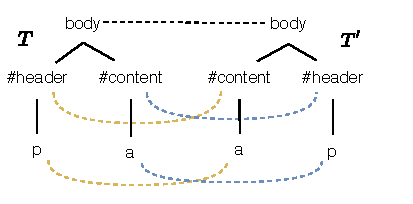
\includegraphics[width=.65\linewidth]{tree-matching/explanation/rted_mistake}
    \caption{Example of matching biased by the TED (as computed by APTED).}
    \label{fig:ted_mistake}
\end{figure}

To address these restrictions when attempting to match two web documents, \cite{fokaefs2011empirical} extended TED with some additional move operations executed \emph{a~posteriori} to address the ancestry restriction and \cite{Kumar2011_FTM,Kumar2011_Bricolage} developed her own \emph{Flexible Tree Matching} (FTM) algorithm to address the ancestry restriction problem.
Unfortunately, while FTM provides a truly restriction-free matching, its high complexity does not allow FTM to scale beyond more than a few dozens of nodes, which is far below the average size of real-life web pages.

% Unfortunately, state-of-the-art algorithms have been proposed to achieve this goal impose to choose between \emph{matching accuracy} or \emph{fast matching}~\cite{xydiff} for any tuple of web documents.
% Furthermore, one can also observe that existing algorithms fail to scale beyond a few hundred of nodes.

% For example, the traditional approach, which is general to any kind of tree, is \emph{Tree Edit Distance} (TED)~\cite{Tai1979} and can be computed in minimum $O(N^3)$ time~\cite{bringmann2018tree}.
% % TED is a restriction of tree matching where descendants of matched nodes can only match with each others (ancestry restriction) and siblings order must be preserved.
% We executed a robust implementation of TED, named APTED~\cite{pawlik2015efficient,pawlik2016tree}, on two instances of the DOM of YouTube, which took more than 4 minutes to propose a matching.
% Unfortunately, when processing and comparing a large dataset of Web documents, one cannot afford such computation times, which makes TED difficult to use in production.

% However, when reproducing this experiment with \textsc{XyDiff},\footnote{\url{https://github.com/fdintino/xydiff}} which is a set of tools for creating and applying deltas from XML documents, results are reported much faster, but the price of a poor accuracy of the resulting tree matchings.

% Figure~\ref{fig:tree_matching_example} illustrates the tree-matching problem. 

% \begin{figure}
%     \centering
% 	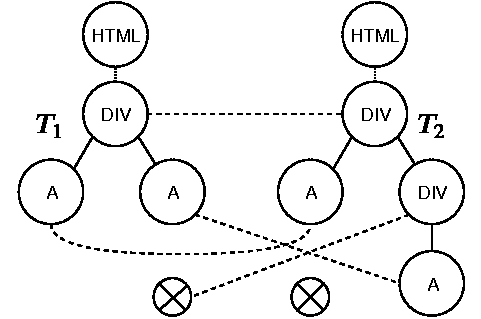
\includegraphics[width=.8\linewidth]{explanation/tree-matching-example}
%     \caption{Example of a tree matching. Crossed circles are auxiliary \emph{no-match} nodes enabling insertions and removals between trees.}
%     \label{fig:tree_matching_example}
% \end{figure}

% The qualitative restrictions or speed limitations of the state of the art therefore led to the development of alternative algorithms.
% For example, \cite{fokaefs2011empirical} extended TED with some additional move operations executed \emph{a~posteriori} to address the ancestry restriction.
% \cite{Kumar2011_FTM,Kumar2011_Bricolage} developed her own \emph{Flexible Tree Matching} (FTM) algorithm to address the ancestry restriction problem, while \cite{reis2004automatic} developed a fast matching system based on top-down matching to extract news faster than TED does. 

In the line of the aforementioned work, this chapter therefore aims at enabling the fast and non-restricted comparison of complex web pages.
In particular, we propose an alternative to the state-of-the-art FTM algorithm, named \emph{Similarity-based Flexible Tree Matching} (SFTM), that leverages similarity metrics to speed up the comparison of complex trees. 
SFTM shares the properties of FTM to offer a non-restricted tree matching, while offering computation times much lower than FTM, even on restricted versions of the problem.
To match two web page trees, the approach taken by SFTM strongly differs from traditional techniques.
In particular, existing matching algorithms are \textit{structure-centric}: they leverage the structure of both trees to select the nodes to visit and compare.
SFTM instead relies on a \textit{label-centric} approach: it prunes the space of possible matchings using nodes' \emph{label} and considers the tree topology \emph{a~posteriori} to propagate information contained in the nodes.
% Furthermore, our algorithm exposes performance parameters to trade computation time and matching accuracy, depending on applications.
% To the best of our knowledge, SFTM is the first solution to match real-life web documents in practical time (\emph{e.g.}, SFTM matches the DOM of YouTube in less than a second compared to 4 minutes for APTED).
% Through empirical evaluation on real websites, we show that our implementation of SFTM qualitatively compares to APTED and scales in $O(n\cdot log(n))$ with the size of the DOM considered in our experiments, thus making it applicable in many production contexts.

We compared SFTM to other state-of-the-art solutions on a large dataset of popular web pages.
SFTM showed almost twice more efficiency than the best existing solution.
Overall, our algorithm SFTM allows to consistently match real-life web pages with high precision (89\% precision on average) in reasonable time (182\,ms on average).

The code for both SFTM and its benchmark is available openly.\footnote{https://anonymous.4open.science/r/7ae57bd7-3b29-463a-88a4-d31c04ecfcd2/}

The remainder of this chapter is organized as follows.
Section~\ref{sec:related_work} and~\ref{sec:ftm} cover related work, with section~\ref{sec:ftm} focusing in details on the \emph{Flexible Tree Matching} (FTM) original algorithm.
Section~\ref{sec:SFTM} presents \emph{Similarity-based Flexible Tree Matching} (SFTM), our extension of FTM that leverages the node labels and local topology similarity to guide the comparison.
Section~\ref{sec:evaluation} thoroughly evaluates our solution against the state of the art on a realistic dataset of web documents.
Section~\ref{sec:threats} discusses the threats to validity of our contribution.
Section~\ref{sec:conclusion} concludes and overviews some perspectives for this work.

\section{Related Work}\label{sec:related_work}
% This section overviews the state of the art in the area of tree matching.
\paragraph{\bf \emph{Tree Edit Distance} (TED)}\label{sec:ted}
Comparing two trees is a problem that has been at the center of a significant amount of research.
In 1979, Tai~\cite{Tai1979} introduced the \emph{Tree Edit Distance} (TED) as a generalization of the standard \emph{edit distance} problem applied to strings.
Given two ordered labeled trees $T$ and $T'$, the TED is defined as the minimal amount of node insertion, removal or relabel to transform $T$ into $T'$, while different cost coefficients can be assigned to each type of operation.
By following an optimal sequence of operations applied to $T$, it is possible to match the nodes between $T$ and $T'$.
This problem has been extensively studied since then to reduce the space and time complexity of the algorithm that computes the TED.
To the best of our knowledge, the reference implementation available today is the \emph{All-Path Tree Edit Distance} (APTED)~\cite{Pawlik2011, pawlik2015efficient, pawlik2016tree} with a complexity of $O(n^2)$ in space and $O(n^3)$ in time in the worst case, where $n$ is the total number of nodes ($n = |T_1|+|T_2|$).
In our work, we consider APTED as one of the baselines to evaluate our contribution.

% \subsection{Restrictions of TED}
\cite{bringmann2018tree} showed that TED cannot be computed in worst-case complexity lower than $O(n^3)$.
In order to circumvent this limitation, several restricted versions of the TED problem have been formulated.
The \textit{Constrained Edit Distance}~\cite{zhang1995algorithms, zhang1996constrained} is an edit distance where disjoint subtrees can only be mapped to disjoint subtrees.
The \textit{Tree Alignment Distance}~\cite{jiang1994alignment} is a TED where all insertions must be performed before any deletion.
The \textit{Top-Down} distance~\cite{selkow1977tree} is computable in $O(|T|\times|T'|)$, but imposes as a restriction that the parents of nodes in a mapping must be in the mapping.
The \textit{Bottom-Up} distance~\cite{valiente2001efficient} between trees builds a mapping in linear time, but such mapping must respect the following constraint: if two nodes have been mapped, their respective children must also be part of the mapping.
\cite{reis2004automatic} proposes a variation of the \textit{Top-Down} mapping, called \textit{Restricted Top-Down Mapping} (RTDM), where replacement operations are restricted to the leaves of the trees, which delivers considerable speed gains, despite a theoretical worst case time complexity still in $O(N^2)$.
By definition TED already sets strong restrictions on produced matchings: sibling order and ancestry relationships must be preserved~\cite{zhang1995algorithms}.
These restrictions are particularly problematic when matching two full web pages together~\cite{Kumar2011_Bricolage}.
While above solutions improve computation times, they answer a restricted version of the TED problem leading to an even more restricted set of possible matchings.

\paragraph{\bf XML\,diff}\label{sec:xmldiff}
While TED-related approaches focus on computing a distance between trees, another part of the scientific literature focuses on inferring the set of edit operations between two XML documents.
Most XML\,diff solutions use an intermediary matching step in order to compute the diff.
Computing the set of diff from a given matching is quite straightforward, which means that most works on the subject actually focus on the matching part.
\textsc{XyDiff}~\cite{Cobena2002DetectingDocuments} matches and computes the diff of two XML documents very quickly.
To do so, \textsc{XyDiff} hashes subtrees from both documents and prunes the space of matching possibilities by matching subtrees with identical hashes.
The algorithm can also make use of id attributes and XSD schemas if they exist.
On the other end of the spectrum, \textsc{X-Diff}~\cite{wang2003x} favors accuracy over speed and computes an optimal matching using hashings of path signatures.
\textsc{XKeyDiff}~\cite{dos2007semantical} builds on \textsc{XyDiff} and adds matching logic based on XML primary keys, \texttt{XML\_SIM\_CHANGE}~\cite{viyanon2010xml} and \texttt{XREL\_CHANGE\_SQL}~\cite{sundaram2012change} match XMLs stored in relational databases using SQL. 
\textsc{Phoenix}~\cite{oliveira2018efficient} interestingly uses a more flexible similarity metric between nodes (\emph{e.g.}, to compare the content of two nodes, they use the \emph{Longest Common Sequence}) and choose how to match each subtree by recursively applying the Hungarian algorithm~\cite{kuhn1955hungarian}.
Unfortunately, \textsc{Phoenix} runs in $O(n^4)$ and yields less accurate results than \textsc{X-Diff}.
In our empirical evaluation, we evaluated our solution along with \textsc{XyDiff}, which is widely known and used for XML\,diff, has an efficient implementation openly available and runs in scalable computation times.

\paragraph{\bf \emph{Flexible Tree Matching} (FTM)}
In~\cite{Kumar2011_Bricolage}, TED is found to be unpractical when applied on DOM, as the resulting matching enforces ancestry relationship---\emph{i.e.}, once two nodes $n, n'$ have been matched, the descendants of $n$ can only be matched with the descendants of $n'$, and \emph{vice~versa}. 
Consequently, Kumar~\emph{et~al.}~\cite{Kumar2011_Bricolage, Kumar2011_FTM} introduced the notion of \textit{Flexible Tree Matching} (FTM), which relaxes the ancestry relationship constraint at the price of a stronger complexity.
It restricts its use to small HTML trees composed of less than a hundred nodes, thus making it unpractical for modern web documents, often including more than a thousand nodes.
Furthermore, to the best of our knowledge, there is no public implementation of FTM that can be considered for comparison.

% \subsection{Limitations \& challenges}
We therefore aim at reducing the complexity of the FTM algorithm in order to scale on complex web pages without enforcing restrictions on produced tree-matching solutions.
While all above contributions are structure-based, we build on FTM's approach and rather offer a flexible, label-based matching where labels are used to match nodes and structure is only used \emph{a~posteriori} to improve the matching.

Our contributions therefore read as follows:
\begin{compactenum}
    \item we develop an algorithm inspired by FTM, coined as \emph{Similarity-based Flexible Tree Matching} (SFTM), by leveraging the notion of label similarity, and similarity propagation to reduce the computation time, and
    \item we apply mutations on real-life web documents to provide a thorough evaluation of our implementation of SFTM, showing that it outperforms state-of-the-art approaches in terms of efficiency.
\end{compactenum}

\section{Flexible Tree Matching (FTM)}\label{sec:ftm}
The \emph{Similarity-based Flexible Tree Matching} (SFTM) we introduce in this chapter can be considered as an extension of the \textit{Flexible Tree Matching} (FTM) algorithm.
This section therefore introduces the FTM algorithm, as originally proposed by Kumar~\emph{et~al.}~\cite{Kumar2011_Bricolage}.
We first describe the notations used throughout the rest of the chapter, and then describe the main steps of the algorithm.

\subsection{FTM Notations and Overview}
We define an ordered tree $T$ as a directed graph $(N,\prec)$ where $N$ is the non-empty set of nodes and $\prec$ a total order relation that can relate a \emph{child} node $c \in N$ to its \emph{parent} $p \in N$, as $c \prec p$, or \emph{siblings}, as $s \in N$, as $c \prec s$.

In particular, we choose a total order rather than a partial one as the order of siblings has a strong semantic value for a webpage (e.g. the order of paragraphs).

In this chapter, we always consider \emph{matchings} between two trees $T=(N,\prec)$ and $T'=(N',\prec')$.

Given two trees $T$ and $T'$, the FTM algorithm relies on the complete bipartite graph $G$ between $N^* = N\cup{\Theta}$ and $N'^* = N'\cup{\Theta}'$, where $\Theta$ and $\Theta'$ are \textit{no-match} nodes.
The fact that $G$ is complete means that every nodes of $T^*$ shares exactly one edge with every nodes of $T'^*$.
Formally, we thus have $E(G) = N^* \times N'^*$ where $E(G)$ are the edges of the graph $G$.
An edge $e=(n, n') \in E(G)$ between $n\in N^*$ and $n'\in N'^*$ represents the matching of $n$ with $n'$. Each edge linking a tuple $(n, n')$ is called a \textit{match}.
So, intuitively, $G$ represents all possible matchings between nodes of $T^*$ and $T'^*$ (cf. Figure~\ref{fig:g_SFTM}).

\begin{figure}
    \centering 
    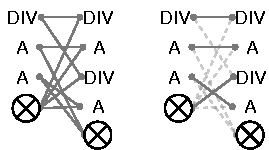
\includegraphics[width=.5\textwidth]{tree-matching/explanation/g_ftm}
    \caption{Building a bipartite graph $G$ representing the set of all possible matchings (left) and then compute the optimal full matching (right).}
    \label{fig:g_SFTM}%
\end{figure}

Formally, we call \textit{matching} and note $M\subset E(G)$, a subset of edges selected from $G$.
A matching $M$ is said to be \textit{full} \emph{iff} each node in $N$ has exactly one edge in $M$ that links it to a node in $N'^*$ and, inversely, each node in $N'$ has exactly one edge in $M$ that links it to a node in $N^*$.
Since matchings need to be \textit{full}, the auxiliary \textit{no-match} nodes $\Theta_1, \Theta_2$ are required to cope with insertion and deletion operations.
The set of possible \textit{full} matchings is restricted to the set of matchings satisfying that every node in $N \cup N'$ is covered by exactly one edge.
\emph{No-match} nodes are the only nodes allowed to be involved in multiple edges.

Given an edge $e=(n, n')\in E(G)$ linking $n$ to $n'$, FTM defines the cost $c(e)$ to quantify how different $n$ and $n'$ are, considering both their labels and the topology of the tree.
Starting from the bipartite graph $G$ describing all possible matchings, the idea behind FTM is to compute the costs $c(e)$ of each edge $e\in E(G)$ and to find the optimal matching with respect to these estimated costs---\emph{i.e.}, to select the set of edges $M\subset E(G)$, such that $M$ is \textit{full} and $c(M)$ is minimal (where $c(M) = \sum_{e\in M}c(e)$).

The upper part of Figure~\ref{fig:steps} describes the main steps involved in computing the final full matching between $T$ and $T'$.

\begin{figure*}
    \centering
	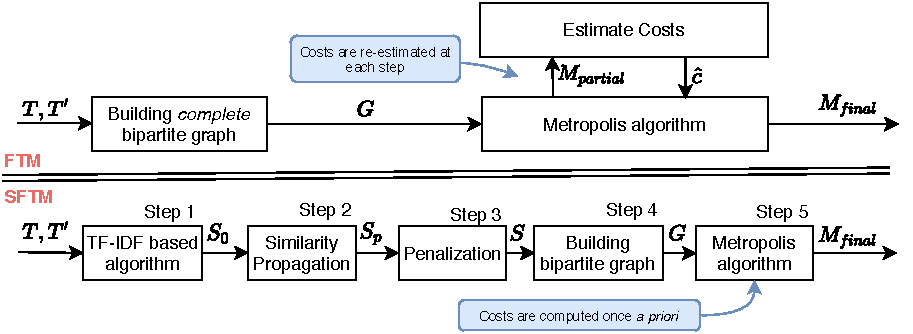
\includegraphics[width=\linewidth]{tree-matching/explanation/ftm-sftm-steps}
    \caption{Steps to compute a full matching between two trees $T$ and $T'$. Upper part covers FTM, while lower part is SFTM.}
    \label{fig:steps}
\end{figure*}

\subsection{Cost Estimation}\label{sec:FTM_cost}
As FTM provides a wide flexibility regarding possible matchings, the design of the cost function $c$ is a key parameter in order to obtain a matching that takes into account both the labels and the topology of the trees.
Typically, the cost $c(e)$ of an edge $e$ between two nodes $n$ and $n'$ is estimated by FTM as follows:
%\text{if }n\text{ or }m\text{ is a no-match node}
\begin{equation}\label{eq:FTM_cost}
c(e) =
\begin{cases}
    w_n                                  & \text{ if}\ n\ or\ n' \in \{\Theta, \Theta'\} \\
    w_r c_r(e) + w_a c_a(e) + w_s c_s(e) & \text{ otherwise}
\end{cases}
\end{equation} 
where $\Theta, \Theta'$ are \textit{no-match} nodes, $w_n$ is the penalty when failing to match one of the edge ends, $c_r(e)$, $c_a(e)$ and $c_s(e)$ are the cost of \textit{relabeling}, \textit{violating ancestry relationship} and \textit{violating sibling group}, respectively, and $w_r$, $w_r$ and $w_r$ their associated weight in the cost function.
$w_n, w_r, c_r, w_a$ and $w_s$ are parameters of the cost function that depend on the kind of matching the user requires.
By extension, we note $c(M) = \sum_{e \in M} c(e)$ the cost of a matching $M$.

Given $e=(n, n')$, the ancestry and sibling costs, $c_a(e)$ and $c_s(e)$, model the changes in topology that matching $n$ with $n'$ entails.
Unfortunately, we can only estimate the costs $c_a$ and $c_s$ if we have access to a full matching, as both costs require a knowledge on how other nodes in the tree were matched (\emph{e.g.}, $c_a$ involves counting the number of children of $n$ matched with nodes that are not children of $n'$).
In order to circumvent the problem, FTM rather considers the approximate costs $\hat{c_a}, \hat{c_s}$ that can be estimated from bounds on the different components of the cost $c$.
Practically, in order to generate one possible full matching, FTM iteratively selects edges in $G$ and, each time an edge is selected, the bounds of $c$ are tightened (we can approximate $c$ more precisely), which means that the costs $\hat{c_a}, \hat{c_s}$ keep being re-estimated along iterations (cf. upper part of Figure~\ref{fig:steps}).
The need to re-estimate the approximated costs after each edge selection actually imposes some critical limitations on the scalability of the algorithm.

\subsection{\textsc{Metropolis} Algorithm}\label{sec:metropolis_ftm}% \cite{Kumar2011_FTM}
Finding the optimal matching, given the graph $G$ and the cost function $c$ is a challenging problem, the authors even proved in~\cite{Kumar2011_FTM} that this problem is NP-hard.
Consequently, the authors described how to use the \textsc{Metropolis} algorithm~\cite{metropolis1953equation} to approximate the optimal matching. 
The \textsc{Metropolis} algorithm provides a way to explore a probability distribution by random walking through samples.
FTM uses this algorithm to random walk through several full matchings, and select the least costly.
The \textsc{Metropolis} algorithm requires to be configured with:
\begin{compactenum}
    \item An initial sample (full matching) $M_0$,
    \item A suggestion function (alternative matching) $M_t \mapsto M_{t+1}$,
    \item An objective function to maximize: $f: M \mapsto \text{quality of } M$,
    \item The number of random walks before returning the best value.
\end{compactenum}

Kumar~\emph{et~al.} defines the objective function $f$ by:
\begin{equation} \label{eq:objective_FTM}
	f_{FTM}(M) = \exp(-\beta\ c(M))
\end{equation}
In order to suggest a matching $M_{t+1}$ from a previously accepted one $M_t$, FTM selects a random number of edges from $M_t$ to keep, sorts remaining edges by increasing costs and iterate through the ordered edges with a probability $\gamma$ to select it.
Once an edge $e = (n,n')$ is selected, all edges connected to $n$ and $n'$ are removed from $G$, and approximate costs need to be re-estimated for all remaining edges, and then sorted so we can select another edge.
The process is repeated until an alternative full matching is obtained.
Therefore, despite using the \textsc{Metropolis} algorithm to reduce the time complexity of the problem, the overall algorithm remains prohibitively costly to compute (cf. Section~\ref{sec:evaluation}), notably due to the continuous re-estimation of the approximated costs at each step of the full matching generation.

\subsection{Complexity Analysis}\label{sec:ftm_complexity}
The original FTM article~\cite{Kumar2011_FTM} does not report on the complexity nor the computation time of the algorithm.
We, therefore, provide an analysis of FTM's theoretical complexity in order to compare it to the one of SFTM (cf. Section~\ref{sec:complexity}).

When discussing complexity, to simplify the notations, we consider the matching of two trees with the same number of nodes and we note $N$ the number of nodes of both trees.

\paragraph{Complete bipartite graph $G$}
Building the complete bipartite graph requires matching each node from $T$ to one node from $T'$, which requires $O(N^2)$ operations. 

\paragraph{\textsc{Metropolis} algorithm}
For each iteration of the \textsc{Metropolis} algorithm, FTM has to suggest a new matching.
In the worst case, the algorithm should choose among all $N^2$ edges.
Each time an edge between $e_1$ and $e_2$ is selected, all other edges connected to $e_1$ and $e_2$ are pruned and remaining costs requires to be re-estimated.
It means that costs have to be re-estimated and sorted for $N^2$ edges, then $(N-1)^2$ edges (after selection and pruning) and so on, until all edges have been selected or pruned.
This implies that the total number of times the costs are re-estimated and sorted is in $O(\sum^N_{n = 0}n^2)$ = $O(N^3)$.
Estimating the cost for a given edge linking $e_1$ and $e_2$ involves counting the number of potential ancestry and sibling violations, which requires going through all edges connected to siblings and children of $e_1$ and $e_2$.
Even if we assume the number of siblings and children is independent from $N$, it still means that estimating the cost of one edge requires $O(N)$ operations.
Thus, in the worst case, the amount of operations required by FTM for each iteration of the \textsc{Metropolis} algorithm is in $O(\sum^N_{n = 0}n^3)$ = $O(N^4)$ (using Faulhaber's Formula).

Overall, the \textsc{Metropolis} step is the one with highest complexity, which means that the complexity of the FTM algorithm is in $O(N^4)$ where $N$ is the number of nodes to match.

% \section{Similarity-based Flexible Tree~Matching}\label{sec:SFTM}
\section{Similarity-based FTM (SFTM)}\label{sec:SFTM}
Based on the above complexity analysis, \emph{Similarity-based Flexible Tree Matching} (SFTM) replaces the cost system of FTM by a similarity-based cost that can be computed once \textit{a~priori} (cf. Figure~\ref{fig:steps}).
This approach drastically improves computation times and rather exposes a parameter that can be tuned to find the desired trade-off between computation time and matching accuracy (cf. Section~\ref{sec:evaluation}).

Given two trees $T=(N,\prec)$ and $T'=(N',\prec')$, SFTM relies on the specification of a \textit{similarity metric} between nodes $n \in N$ and $n' \in N'$.
We compute this similarity metric for all pairs of nodes $(n,n')$ using \emph{i)} inverted indices for labels and \emph{ii)} label propagation and some penalization heuristics for the topology.
We build a bipartite graph $G$ between nodes of $T$ and $T'$ using this similarity metric to compute the costs and apply the Metropolis algorithm to approximate the optimal full matching from $G$.
This new similarity measure allows SFTM to improve the FTM algorithm in two key aspects:
\begin{compactenum}
	\item when building $G$, we do not create all $|N|\times|N'|$ possible edges. We only consider edges linking two nodes with a non-null similarity; and
    \item when generating a full matching, costs do not need to be updated as these costs solely depend on our similarity measure.
\end{compactenum}
In this section, we therefore
\begin{inparaenum}[(a)]
	\item introduce our new similarity metric, and
    \item describe how we leverage it to approximate the optimal full matching.
\end{inparaenum}

\subsection{Overview of Similarity-based Matching}\label{se:newCost}
The similarity metric between nodes $N$ and $N'$ is computed in two main steps:
\begin{inparaenum}
	\item we compute $s_0$, the initial similarity function using only \textit{labels} of the trees individually, and then
    \item we transform $s_0$ to take into account the topology of the tree and compute our final similarity function $s$.
\end{inparaenum}
The computation of $s_0$ leverages inverted index techniques traditionally used to query text in a large document database.
In our case, the documents we query against are $N$, while queries are extracted from $N'$.
Figure~\ref{fig:steps} illustrates the different steps described in this section.

\subsubsection{Initial Similarity (step\,1)}
To compute the initial similarity $s_0$ between $N$ and $N'$ (cf. \textit{step 1} in Figure~\ref{fig:steps}), we independently compare the labels of $N$ and $N'$ using the \emph{Term Frequency-Inverse Document Frequency} (TF-IDF).
The resulting initial node similarity $s_0$ does not take the topology of the trees into account.

In order to take into account relabeling cost between nodes, some existing solutions (\emph{e.g.}, APTED) allow the user to input a pairwise comparison function $label(n), label(m) \mapsto similarity\ score$.
However, computing this similarity score for all the pairs of nodes requires $O(N^2)$ operations.
Thus, to reduce the number of operations, SFTM uses---instead---inverted indices: given a tokenize function $tokenize : n \mapsto \ token\ list$, SFTM
\begin{inparaenum}
	\item decomposes each node $n$ from $N$ into a set of tokens (as defined by the $tokenize$ function), and then
    \item iterates through tokens of nodes $n'$ from $N'$ to increase the value of $s_0(n,n')$ for each token $n$ and $n'$ have in common.
\end{inparaenum}
Section~\ref{tokenSelection} provides a detailed description of the function $tokenize$ we use in our evaluation.

Decomposing nodes from $N$ into tokens allows SFTM to build an inverted index $TM$ (\emph{Token Map}), which maps every token $tk$ with the list of nodes of $N$ that contains $tk$.
The idea behind the inverted index $TM$ is to use the information that a node $n \in N$ contains a token as a differentiating feature of $n$ allowing to quickly compare it to nodes in $N'$.
If a token $tk$ appears in all nodes $N$, this token has no differentiating power.
In general, the rarest a token, the more differentiating it is.
This idea is very common in \emph{Natural Language Processing} (NLP) and a common tool to measure how rare is a token in TF-IDF~\cite{jones1972statistical} and more precisely, the \emph{Inverted Document Frequency} (IDF) part of the formula.
Applying TF-IDF to our similarity yields the following definition:
\begin{align}
	IDF(tk) &= log(|N|/|TM[tk]|) \\
	s_0(n,n') &= \sum_{tk \in TK}IDF(tk)
\end{align}
Where $TK=tokens(n) \cap tokens(n')$.
The function IDF is a measure of how rare a token is, $|TM[tk]|$ is the number of nodes containing the token $tk$ and $tokens$ refers to the user input tokenize function.
Intuitively, we retrieve the tokens shared between nodes $n$ and $n'$ and, for each common token $tk$, we increase $s(n,n')$ by a high value if $tk$ is rare and a low value if $tk$ is common.
In Section~\ref{sec:implementation}, we provide a detailed implementation of how to compute the initial similarity $s_0$.

Tokens that appear in many nodes have little impact on the final score---\emph{i.e.}, low IDF---yet have a very negative impact on the computation time.
In our algorithm, we expose the sublinear threshold function $f: N \mapsto f(N) < N$ as a parameter of the algorithm.
We use $f$ to filter out all the tokens appearing in more than $f(N)$ nodes.
Therefore, $f$ provides a balance between computation time and matching quality: when $N-f(N)$ decreases, computation times and matching quality increase.
In Section~\ref{sec:complexity}, we discuss how $f(N)$ influences the worst-case theoretical complexity.
% An exhaustive theoretical and empirical analysis of precisely how $f$ influences the computation times and matching quality will be the object of future studies.

\subsubsection{Local Topology (step\,2)}
$s_{0}$ represents the similarity between node labels, but does not take into account the topology of the trees.
To weight in local topology similarities, we propagate the score of each node pair to their offspring and siblings.
This idea of propagation is inspired by recent \emph{Graph Convolutional Network} (GCN) techniques~\cite{kipf2016semi}.

The original FTM algorithm includes two terms in the cost function, $c_a$ (ancestry cost) and $c_s$ (sibling cost), which reflect the topology of the trees.
Since we do not use these terms (as they require too much computation time), we need our similarity score to reflect both the similarity of node labels and the similarity of the local topology.
Therefore, we first compute the score matrix $s_0$, based on the label similarity we described above, and then we update this score to take into account the matching score of the parents of $n$ and $n'$.
By doing so, $n$ has a higher similarity score with $n'$ if their respective parents or children are also similar.

Beginning at $s_0$, at each step $i$ and for all pairs that have a non-null initial score  $\{(n, n')\in N \times N' | s_0 \neq 0\}$, we first compute:
\begin{equation}\label{eq:score}
	s_{i}(n, n') \gets s_{i-1}(n, n') +  w_i \times s_{i-1}(p(n), p(n'))
\end{equation}
where $p(n) \in N$ refers to the parent of node $n$.

Similarly, we then increase the score of the parents of $n, n'$:

\begin{equation}\label{eq:score_parent}
	s_{i}(p(n), p(m)) \gets s_{i-1}(p(n), p(n')) +  v_i \times s_{i-1}(n, n')
\end{equation}
where $w_0, w_1\dots w_{P}$ and $v_0, v_1 ... v_P$ are topology weights.
We repeat the process $P$ times ($P$ for propagation) where $P$ is a parameter of SFTM.
The resulting function $s_{P}$ then reflects both label similarity and local topology similarity.

Intuitively, at each iteration, we propagate information further up in the tree.
This is why, the weight sequences $w$ and $v$ should be decreasing so that close kinship among nodes prevails.
From our experiments, we advice the following values for the $P=3$ weights: $w_0 = 0.4, w_1 = 0.04, w_2 = 0.004$ and $w_0 = 0.8, w_1 = 0.08, w_2 = 0.008$.
These values were used and unchanged for all results presented in the empirical evaluation~\ref{sec:evaluation}, leading to high accuracy on a large variety of web documents.

\subsubsection{Penalization (step\,3)}
There are two main drawbacks to the way we propagate the scores in step\,2:
\begin{inparaenum}
\item the scores are still almost exclusively based on labels,
\item nodes with many children may get an unfair score boost from the propagation.
\end{inparaenum}

While (2) can be fixed by normalizing the propagation according to the number of children, the normalization would also potentially remove valuable information.
Instead, for each pair $(n,n')$, we rather apply a penalization proportional to the difference between the number of children of $n$ and $n'$:
\begin{equation}
s(n,n') = s_{P} \times (1 - penalty(n,n'))
\end{equation}
where $penalty(n,n') \mapsto [0, 1]$ is the children penalization defined by:
\begin{equation}
penalty(n,n') = \frac{|(|children(n)|-|children(n')|)|}{max(|children(n)|,|children(n')|)}
\end{equation}
where $|ch(n)|$ is the number of children nodes of $n$.
This step yields the final score function $s$, defined for each couple $(n,n')$.

\subsubsection{Building the bipartite graph $G$ (step\,4)}
Using our final score function $s$, we can now build the bipartite graph $G$: we iterate over all nodes $n \in N$ and we create an edge $e=(n,n')$ for each pair of nodes such that $s_{P}(n,n') \neq 0$ and associate it with the cost $c(n,n') = 1/(1+s_{P}(n,n'))$.
Our resulting cost function is thus defined as follows:
\begin{equation}\label{eq:SFTM_cost}
c_{SFTM}(e) =
\begin{cases}
w_n,                    & \text{if }n\text{ or }n'\text{ is a no-match node}\\
\frac{1}{1+s_{p}(n,n')},& \text{otherwise}
\end{cases}
\end{equation}

Importantly, unlike the bipartite graph built in the FTM algorithm, the resulting bipartite graph $G_{SFTM}$ is \emph{not complete} as only edges, such that $s_{p}(n,n') \neq 0$ are considered.
This is one of the key differences allowing SFTM to drastically improve computation times.

\subsection{Implementation Details}\label{sec:implementation}
In the previous section, we introduced the SFTM algorithm and described how it compares to FTM.
In this section, we describe more precisely how we implement the different steps of SFTM.  

\subsubsection{Node Similarity (step 1, 2 and 3)}
Let us consider two trees $T$ and $T'$.
We first build the dictionary $TM$, an inverted index---\emph{i.e.}, each entry of $TM$ is a tuple $(token, nodes)$ where $token$ is a token (usually a string) and $nodes$ is a \textit{set} of all $n \in N$ that contains $token$.
Figure~\ref{fig:inverted_index} (2a,b) depicts two examples of inverted index.
We note $TM{map}[key]$ the set of $nodes$ whose key in $TM$ is $key$.
In Section~\ref{tokenSelection}, we further describe how we sort HTML nodes into tokens.

\begin{figure*}
    \centering
    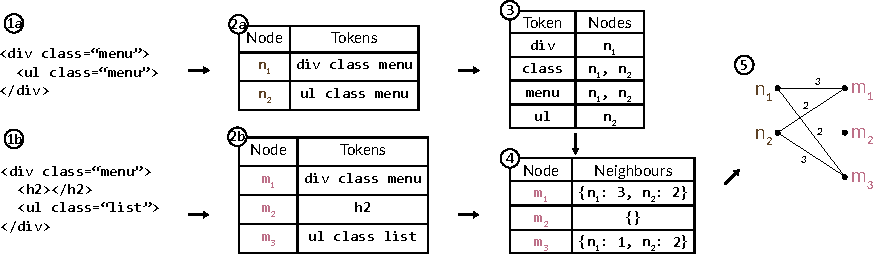
\includegraphics[width=\linewidth]{tree-matching/explanation/inverted_index}
    \caption{Creating the bipartite graph $G$ from two example DOMs $T,T'$. (1a,b)~are the input DOMs, (2a,b)~the extracted tokens, (3)~the inverted index $TM$, (4)~the neighbours dictionaries, and (5)~the resulting bipartite graph $G$. For simplicity, the figure shows a matching where $IDF(tk)=1$, $P=0$ and no-match nodes are not displayed.}\label{fig:inverted_index}
\end{figure*}

Given the inverted index $TM$, we define the function $IDF: tk \mapsto log(|N|/|TM[tk]|)$.
In order to limit the complexity of our algorithm, we remove every token $tk \in TM$ that is contained by more than $f(N)=\sqrt{N}$ nodes, where $f$ is the chosen sub-linear threshold function.
This is equivalent to putting a threshold on $IDF$ to only keep tokens $\{tk \in TM |IDF(tk) > log(\sqrt{N})\}$.
Removing the most common tokens has a limited impact on matching quality, since these are exactly the tokens that provide the least information on the nodes they appear in.

% \begin{algorithm2e}
% \SetAlgoLined
% \KwIn{\\
% n': a node in $N$\\
% $TM$: token map, dictionary of nodes from $T$ per token
% }
% \KwResult{neighbors: a dictionary of scores per node in $T$}
% $neighbors \gets new\ Dictionary()$\\
% \ForEach{tk in tokens(n')} {
%     \ForEach{$n$ in $TM[tk]$} {
%         $neighbors[n] += IDF(tk)$\\
%     }
% }
% \Return neighbors
% \caption{For a given node $n'\in N'$, compute similarity score $s_0(n,n')$ with all $n\in N$, such that $s_0 > 0$}\label{scoreAlgo}
% \end{algorithm2e}

Once we have the token index $TM$ and the function $IDF$, we apply Algorithm~\ref{scoreAlgo} on each node $n' \in N'$.
In Algorithm~\ref{scoreAlgo}, we first compute the tokens of node $n'$ and, for each token $tk$, we use $TM$ to retrieve the nodes $n \in N$ that contain the token $tk$.
Each node $n$ thus retrieved is considered as a \textit{neighbor} of $n'$---\emph{i.e.}, $s_0(n,n') \neq 0$.
Finally, for each neighbour $n$ of $n'$, we add $IDF(tk)$ to the current score $s_0(n,n')$.
At this point, we have a $neighbors(n')$ dictionary for each node $n' \in N'$.
Each $neighbors(n')$ dictionary contains all non-null matching scores: $\forall n \in keys(neighbors(n')), neighbors(n')[n] = s_0(n,n')$.
Using the Equation~\ref{eq:score}, we can now easily compute $s_{p}$ and $s$.

\subsubsection{Building the Token Vector}\label{tokenSelection}
The actual labels are never directly used by SFTM. The algorithm only leverages the tokens extracted from these labels. The way we choose to extract the tokens contained in a node $n$ thus strongly influences the quality of our similarity score.
% Finding the optimal way to compute these tokens has been the topic of extensive studies~\cite{christen2011survey, steorts2014comparison, datar2004locality}.
We implemented the following function $tokens$ to report all the tokens of a node $n$.
Given $n$, an HTML node representing a \texttt{tag}:
\begin{verbatim}
  <tag att_1="val_1" ... att_2="val_2">
    CONTENT
  </tag> 
\end{verbatim}
where $l$ is the number of attributes, $(att_i, val_i), i \in [1,l]$ are the attribute/value pairs of $n$ and the absolute XPath of $n$ is $xPath(n)$.
We decompose $n$ into the following tokens:
\begin{equation}
	tokens(n) = \{xPath(n), \texttt{tag}, att_1..a_l, tok(val_1)..tok(val_l)\}
\end{equation}
where $tok$ is a standard string tokenizing function that takes a string and splits it into a list of tokens on each non Latin character.
The absolute XPath of a node $n$ in a tree is the full path from the root to the element where ranks of the nodes are indicated when necessary---\emph{e.g.}, \texttt{html/body/div[2]/p}.

SFTM does not include the text content of the nodes in the extracted token vectors.
This decision allow to match pages in different languages or containing different content (e.g. news website) in a robust way.

\subsubsection{Building G (step\,4)}
Using Equation~\ref{eq:SFTM_cost}, we compute the cost $c(n,n')$ for each couple $(n,n')$ where $s_p(n,n') \neq 0$.
Then, for each node $n'\in N'$, we add one edge for all nodes $values(neighbours(n')) \subset N$.

\subsubsection{Metropolis Algorithm (step\,5)}
Once we built the graph $G$ with its associated costs, we need to find the set of edges $M$ in $G$ that represents the best full matching between $T$ and $T'$.
In order to do so, we apply the \textsc{Metropolis} algorithm in a different way than FTM does: 
\begin{inparaenum}
	\item we adopt an alternative objective function, and
    \item SFTM matching suggestion function is faster to compute, as costs never need to be re-estimated.
\end{inparaenum}

Typically, FTM uses the objective function $f_{FTM}(M) = \exp(-\beta\ c(M))$.
In the original FTM article, the authors noted that the parameter $\beta$ seemed to depend on $|M|$.
In order to avoid this dependency, we therefore normalize the total cost:
\begin{equation}
	f_{SFTM}(M) = \exp(-\beta\ \frac{c(M)}{|M|})
\end{equation}
The function $suggestMatching: M_i \mapsto M_{i+1}$ takes a full matching $M_i$ and returns a full matching $M_{i+1}$ related to $M_i$.
In Algorithm~\ref{suggestMatching}, 
\begin{compactenum}
	\item $selectEdgeFrom(edges)$ loops through $edges$ (in order) and, at each iteration $j$, has a probability $\gamma \in [0,1]$ to stop and return $edges[j]$,
    \item $connectedEdges(edge)$, where $edge$ connects $u$ and $v$, returns the set $E$ of all edges connected to $u$ or $v$ (note that $edge \in E$).
\end{compactenum}

% \begin{algorithm2e}
% \SetAlgoLined
% \KwData{$G$ : The bipartite graph}
% \KwIn{$M_i$: A full matching}
% \KwResult{$M_{i+1}$: the suggested full matching}
%  $M_{i+1} \gets []$  \\
%  $remainingEdges \gets sortedEdges(g)$ \\
%  $toKeep \gets randomInt(0, |M_i|)$ \\
%  \For{j = 0 ... toKeep}{
%     edge $\gets$ remainingEdges.first \\
%  	$M_{i+1}$.add(edge)\\
%     remainingEdges.removeAll(connectedEdges(edge))
%  }
%  \While{$remainingEdges$ is not empty} {
%     $edge \gets selectEdgeFrom(remainingEdges)$ \\
%     $M_{i+1}$.add(edge)\\
%     remainingEdges.removeAll(connectedEdges(edge))
%  }
%  \Return $M_{t+1}$
%  \caption{Suggest a new matching}\label{suggestMatching}
% \end{algorithm2e}

In practice, we first compute all the connected nodes and edges before storing them as dictionaries, so that the function $connectedEdges$ in Algorithm~\ref{suggestMatching} can be computed in $O(1)$ time.
It is worth noting that, to allow fast removal, the list $remainingEdges$ is implemented as a double-linked list.
The parameter $\gamma$ defines a trade-off between exploration (low $\gamma$) and exploitation (high $\gamma$).
For the Metropolis related parameters, we used mostly the values advised in the original FTM article~\cite{Kumar2011_FTM}: $\gamma = 0.8, \beta = 2.5$ and a number of iterations of 10.

\subsection{Complexity Analysis}\label{sec:complexity}
We are interested in evaluating the time complexity of the algorithm with respect to the size of both trees $N$.
In our analysis, we consider that $N_{tk}=max(|tokens(n)|, n \in nodes(T))$, the maximum number of tokens per node is a constant since it does not evolve with $N$.

When building $G$, we first compute the inverted index $TM$, which requires to iterate through the tokens of all the nodes in $T$, and thus implies a complexity in $O(N \cdot N_{tk}) = O(N)$.

To find the neighbours of nodes from $T'$ using $TM$, we iterate through all the nodes in $T'$, while each node in $T'$ has $N_{tk}$ tokens.
The number of nodes containing a token is artificially limited to $f(N)$.
Thus, building the similarity function $s_0$ takes $O(N \cdot f(N))$ time.

For each node $n'$ in $T'$, we create an edge for each neighbor $n$ of $T$.
Each token $tk \in tokens(n')$ adds up to $f(N)$ neighbors.
It means that the total number of edges is in $O(N \cdot N_{tk} \cdot f(N))$ = $O(N \cdot f(N))$.

Before executing the \textsc{Metropolis} algorithm on $G$, we sort all the edges by cost, which takes $O(N \cdot f(N) \cdot log(N \cdot f(N))) = O(N \cdot f(N) \cdot log(N))$ (as $f(N) \leq N$).
Finally, at each step of the \textsc{Metropolis} algorithm, we run the $suggestMatching$ function, which prunes a maximum of $O(f(N))$ neighbors for each one of the $N$ edges it selects.

Overall, sorting all edges requires the highest theoretical complexity: $O(N \cdot f(N) \cdot log(N))$.
If no threshold is set---\emph{i.e.}, $f(N) = N$---then the worst-case overall complexity of SFTM is $O(N^2 \cdot log(N))$, which keeps outperforming TED ($O(N^3)$) and FTM ($O(N^4)$).

In this evaluation, we used $f(N) = \sqrt{N}$, which leads to a theoretical worst-case complexity in $O(N \cdot \sqrt{N} \cdot log(N))$.
% The empirical evaluation conducted in Section~\ref{sec:evaluation} tends to suggest that the average-case complexity may be even lower in practice.

\section{Empirical Evaluation}\label{sec:evaluation}
The objective of this evaluation is to assess that:
\begin{compactenum}
	\item the quality of the matchings reported by SFTM compares with the baselines we selected---APTED and \textsc{XyDiff}---and
    \item SFTM offers practical computation times on real-life web pages.
\end{compactenum}

\subsection{Input Web Document Dataset}
We need to assess the ability of SFTM to match the nodes between two slightly different web pages $d$ and $d'$.
To measure and compare the accuracy of all studied solutions, we must have access to the ground truth matching between $d$ and $d'$---\emph{i.e.}, for each node $n$ in $d$, what is the true matching node $n'$ in $d'$.

To the best of our knowledge, there is no established and public benchmark that include such pairs of trees, along with the ground truth matching of their nodes. Creating such a benchmark is challenging.
Existing matching solutions usually do not provide any qualitative empirical benchmark~\cite{Bunke1998ASubgraph,Dinitz1998OnIsomorphism, jiang1994alignment,valiente2001efficient,Wang2001FindingHierarchy,zhang1995algorithms} and challenging matching problems involve thousands of nodes, which makes manual labeling error prone for humans (both trees could not even be rendered on the same screen).
Therefore, we built a a semi-synthetic dataset built from mutations applied to real-life web pages, thus obtaining a large-scale dataset in which the ground truth is known.

\paragraph{DOM mutation}
To build a grounded dataset of $(d,d')$ pairs---\emph{i.e.}, where the ground truth (perfect matching) is known---we developed a mutation-based tool that operates as follows:
\begin{compactenum}
	\item we construct the DOM $d$ from an input web document,
    \item for each element of $d$, we generate a unique signature attribute,
    \item for each original DOM $d$, we randomly generate a set of mutated versions: the \textit{mutants}.
    Each \textit{mutant} $d'$ is stored along with the precisely described set of mutations that was applied to $d$ to obtain $d'$.
    Importantly, the signature tags of the elements in $d$ are transferred to $d'$, which constitutes the perfect matching between $d$ and $d'$. These signatures are obviously ignored when applying the matching algorithms.
\end{compactenum}

In our tool, most attention has been dedicated to the choice of relevant mutations to apply.
We therefore relied on the expertise of web developers to identify the most common changes that can apply to DOM.
Their feedback led to the identification of the following list of mutation operations:
% \begin{center}
%   \begin{tabular}{|l l|} 
%       \hline
%       Element       & Mutation operators\\
%       \hline
%       \hline
%       \em Structure & \tt remove, duplicate  wrap, unwrap, swap \\
%       \em Attribute & \tt remove, remove words \\
%       \em Content   & \tt replace with random text, change letters, \\
%                      & \tt remove, remove words \\
%       \hline
%   \end{tabular}
% \end{center}

\begin{center}
    \begin{table}[h]
    \begin{tabular}{l|l}
    \hline
    Category  & Mutation Operators                       \\ \hline
    Structure & \tt Remove, duplicate, wrap, unwrap, swap    \\
    Attribute & \tt Remove, remove words                     \\
    Content   & \tt Replace, remove, remove words, change letters \\ \hline
    \end{tabular}
    \end{table}
\end{center}
where
\textit{Structure: remove} removes an element and its children (recursively), 
\textit{duplicate} duplicates a subtree, applies $mutate$ to duplicated subtree and insert the subtree anywhere in the tree,
\textit{wrap} wraps an element within a new $div$ container,
\textit{unwrap} removes an element $e$ and attach the children of $e$ to the parent of $e$,
\textit{swap} swaps the position of two sibling elements,
\textit{Attribute: remove} removes an attribute with its value,
\textit{Attribute: remove words} removes a random number of tokens from the value of an attribute,
\textit{Content: replace} replaces the content of an element with a random text whose size is close to the original,
\textit{Content: change letters} replaces a few letters in the content of an element,
\textit{Content: remove} removes the content of an element,
\textit{Content: remove words} removes random tokens from the content of an element.

We believe that the above mutations are representative of a wide range of changes that apply in web pages, although they may not perfectly cover all the cases encountered in practice.
In particular, the distribution of these mutations might not be uniform in real life---\emph{i.e.} some mutations might happen more than others.
Yet, this evaluation intends to compare the sensitivity of studied matching algorithms to common mutations, which remains a relevant context to estimate and compare their quality.

\paragraph{Input document sample}
We fed our mutation tool with the home pages of the Top\,1K Alexa websites.\footnote{https://www.alexa.com/topsites}
Alexa provides a list of websites ordered by popularity, thus providing a representative list of web pages of variable complexities.
For each original DOM $d$, we created $10$ mutants $d'_0\dots d'_9$ with a ratio of mutated nodes ranging from $0$ to $50\%$ of the total number of nodes on the page, $|nodes(d)|$.

Overall, we obtained a dataset composed of $6,276$ document pairs $d,d'_n$ that could be correctly processed by the algorithms under study.
Figure~\ref{fig:distribution} reports on the size distribution, in number of nodes, of original and mutated web documents included in this dataset.

\begin{figure}
    \centering
    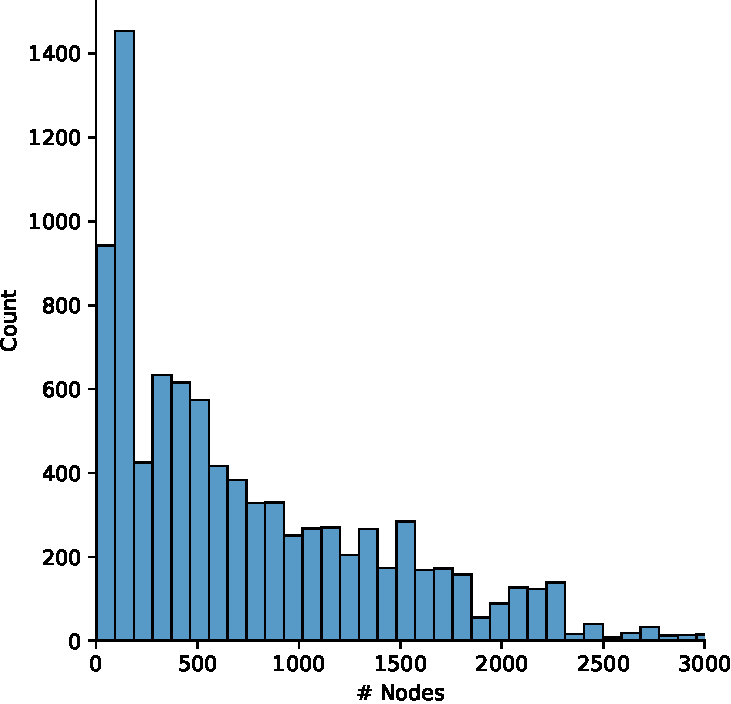
\includegraphics[width=.6\linewidth]{tree-matching/graphs/distribution_size}
    \caption{Distribution of DOM sizes (in terms of nodes) in the dataset.}
    \label{fig:distribution}
\end{figure}

\subsection{Baseline algorithms}
Given no implementation of the original FTM algorithm is available, we implemented and evaluated it, but the computation times and space complexity of this implementation were too high to run the algorithm on real-life web documents (\emph{e.g.} for a tree of 58 nodes, the computation took 1 hour).

We thus mainly compare SFTM to APTED and \textsc{XyDiff}.
APTED is the reference implementation of TED that reports on the best performance so far.
The implementation of APTED used for this evaluation is the one provided by the authors of~\cite{pawlik2016tree,pawlik2015efficient}.
Since APTED yields the optimal solution to the TED problem, TED is theoretically superior in accuracy to all more restricted solutions (see Section~\ref{sec:related_work}).

\textsc{XyDiff} is the most widely-known and used algorithm to efficiently match XML documents. Unlike APTED, XyDiff does not return an optimal result, it instead focuses on speed which makes it a complementary candidate to APTED as a baseline. 
In order to use \textsc{XyDiff} on HTML pages we had to convert the HTML into XHTML, which mostly means closing unclosed tags (\emph{e.g.}, input tags).
We used an existing open source implementation of \textsc{XyDiff}.\footnote{https://github.com/fdintino/xydiff}
We consider the pairs $(d,d')$ taken from the above input dataset, and we systematically ran SFTM, APTED, and \textsc{XyDiff} algorithms with each pair to match $d$ with $d'$ on the same machine.

\paragraph{Ground truth}
When building the dataset, we keep track of nodes' signature so that we always know which nodes from $d$ should match with nodes from $d'$.
This ground truth is hidden from the evaluated algorithms, but is used \emph{a~posteriori} to measure and compare the quality of the matchings computed by the algorithms under evaluation.
% Our purpose in this section is not to conduct a thorough qualitative comparison of the algorithms, since it would require optimizing the parameters of both algorithms in an unbiased way.
% Instead, we show that SFTM returns qualitatively comparable results, while drastically reducing computation time.

\subsection{Experimental Results}\label{sec:performances}
All the results in this section have been obtained by running all three algorithms on the same server containing 252\,GB of RAM and an Intel(R)~Xeon(R) CPU E5-2660\,v3 @ 2.60\,GHz.

\paragraph{Matching quality}
The signature tags injected in nodes from $d$ and $d'$ allow us to assess the quality of the matchings by comparing to the ideal matching $M_{ideal}$.
For the qualitative analysis, we model the tree matching algorithm as a binary classification problem: Given two trees $T$ and $T'$ containing the set of nodes $N$ and $N'$ respectively, $N \times N'$ is the set of all possible matches.
We consider the matching $M_a \subset N \times N'$ produced by a tree matching solution $a$.
Then, a match $e=(n,n') \in M$ is classified as positive by $a$ if $e \in M_a$.
All matches that should be positive are in the ideal matching $M_{ideal}$.
All possibilities are summarized in the following confusion matrix:
\begin{center}
    \begin{tabular}[h]{l|c|c|}
    % \hline
    \cline{2-3} 
    
                                          & $e \in M_{ideal}$ & $e \notin M_{ideal}$ \\
    % \cline{2-3}
    % \cline{1-3}
    \hline
    \multicolumn{1}{|l|}{$e \in M_a$}    & \textbf{True Positive} & False Positive\\
    \hline
    \multicolumn{1}{|l|}{$e \notin M_a$} &         False Positive & \textbf{True Negative}\\
    \hline
    \end{tabular}
    % \caption{Confusion matrix modeling the evaluation of SFTM as a binary classification problem}
\end{center}

Using the above confusion matrix, we can compute the \textit{precision}, \textit{recall}, metrics and the \textit{F1 score}, which are very commonly considered for binary classification problems.

Figure~\ref{fig:f1score} reports on the precision, recall and F1 score of the 3 tree matching solutions we compared, namely SFTM, APTED, and \textsc{XyDiff}.
As expected, the accuracy of all solutions decreases when the mutation ratio increases.
However, for all the reported metrics, SFTM clearly outperforms both \textsc{XyDiff} and APTED.
For both APTED and \textsc{XyDiff}, we believe the lack of accuracy stems from the lack of flexibility when matching labels.
\textsc{XyDiff} relies entirely on hashing subtrees of the document and match subtrees with identical hash.
While this approach might be robust to small structural mutations, it is naturally very sensitive to large amounts of mutations when both structures and labels are mutated.
Similarly, TED compares the labels of most pairs of nodes and generate an associated cost of \texttt{1} when the labels are identical and \texttt{0} when they are different (no gradual costs if the labels are similar).
% We modified the cost function on APTED to provide a more flexible label cost function.
% The accuracy obtained was better (equivalent to SFTM) but the computation times were prohibitive (4 minutes to match youtube pages) which is understandable since this comparison function runs $O(n^3)$ times.
% For this reason, we could only run the modified version of APTED on a few hundred small pages and the results presented in Figure~\ref{fig:f1score} reports on the non-modified version.

\begin{figure}
  \centering
  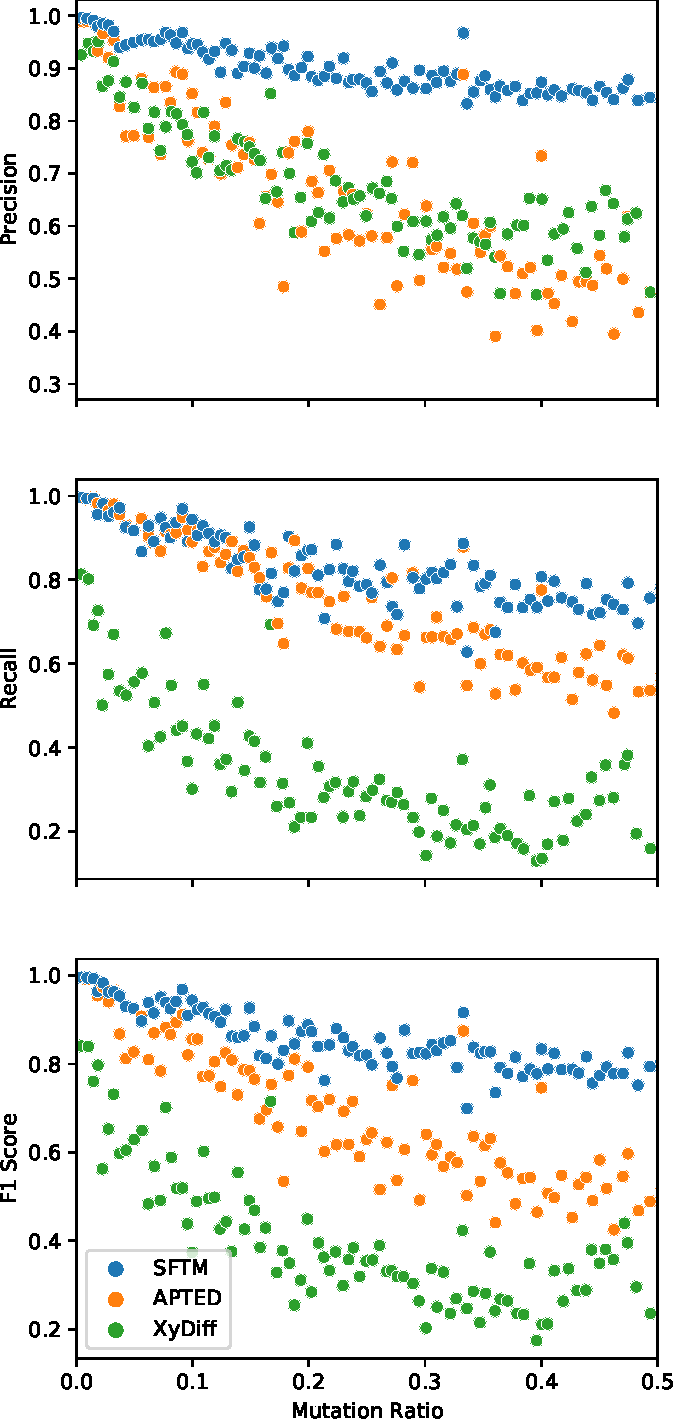
\includegraphics[width=.65\linewidth]{tree-matching/graphs/f1score}
  \caption{Precision, Recall, and F1 Score of SFTM, APTED, and \textsc{XyDiff}.}
  \label{fig:f1score}
\end{figure}

\paragraph{Completion time}
For each couple ($d$, $d'$) retrieved from the dataset, we measured the time taken by SFTM, APTED, and \textsc{XyDiff} to compute a full matching.
Figure~\ref{fig:computation_time} reports on the average time to match DOM couples of increasing size (in terms of number of nodes) for all three solutions.
\textsc{XyDiff} exhibits very fast computation speed and despite its numerous optimizations, APTED's computation times increases exponentially large web documents.
SFTM is not as fast as \textsc{XyDiff}, but seems to show reasonable growth when the size of web documents increases.
Interestingly, APTED computation time varies greatly, which is due to the multiple heuristics used by this implementation to optimize the computation in certain situations.

\begin{figure}%{\textwidth}
    \centering
    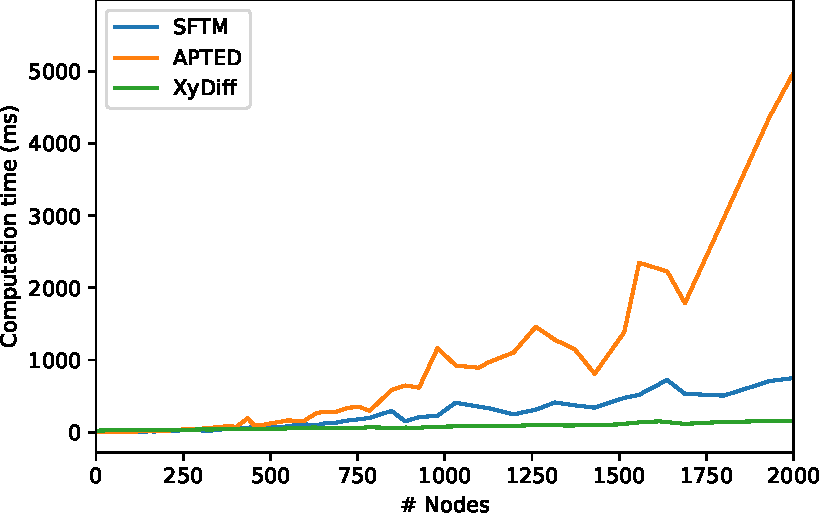
\includegraphics[width=.85\linewidth]{tree-matching/graphs/computationTime}
    \caption{Computation times when matching trees of different sizes.}
    \label{fig:computation_time}
\end{figure}%

Overall, one can observe that SFTM offers an interesting trade-off between two classes of tree matching algorithms: the ones maximizing accuracy at the cost of time, like APTED, and those minimizing the completion time at the cost of reduced accuracy, like \textsc{XyDiff}.

% Figure~\ref{fig:sftm_speed} delivers a closer look on the scalability of SFTM.
% The empirical results seem to indicate an evolution in $O(n \cdot log(n))$: in  Figure~\ref{fig:sftm_speed}, we replaced the X axis from the number of nodes in the DOM $n$ to $n\ log(n)$ then computed a linear regression on the curve which resulted in a correlation coefficient $r^2 = 86\%$.
% We believe the complexity depends on the distribution of nodes within the tokens and a more thorough theoretical analysis will be conducted in the future to understand the gap with the theoretical complexity (cf. Section~\ref{sec:complexity}). 

    % \begin{figure}%{\textwidth}
    %     \centering
    %     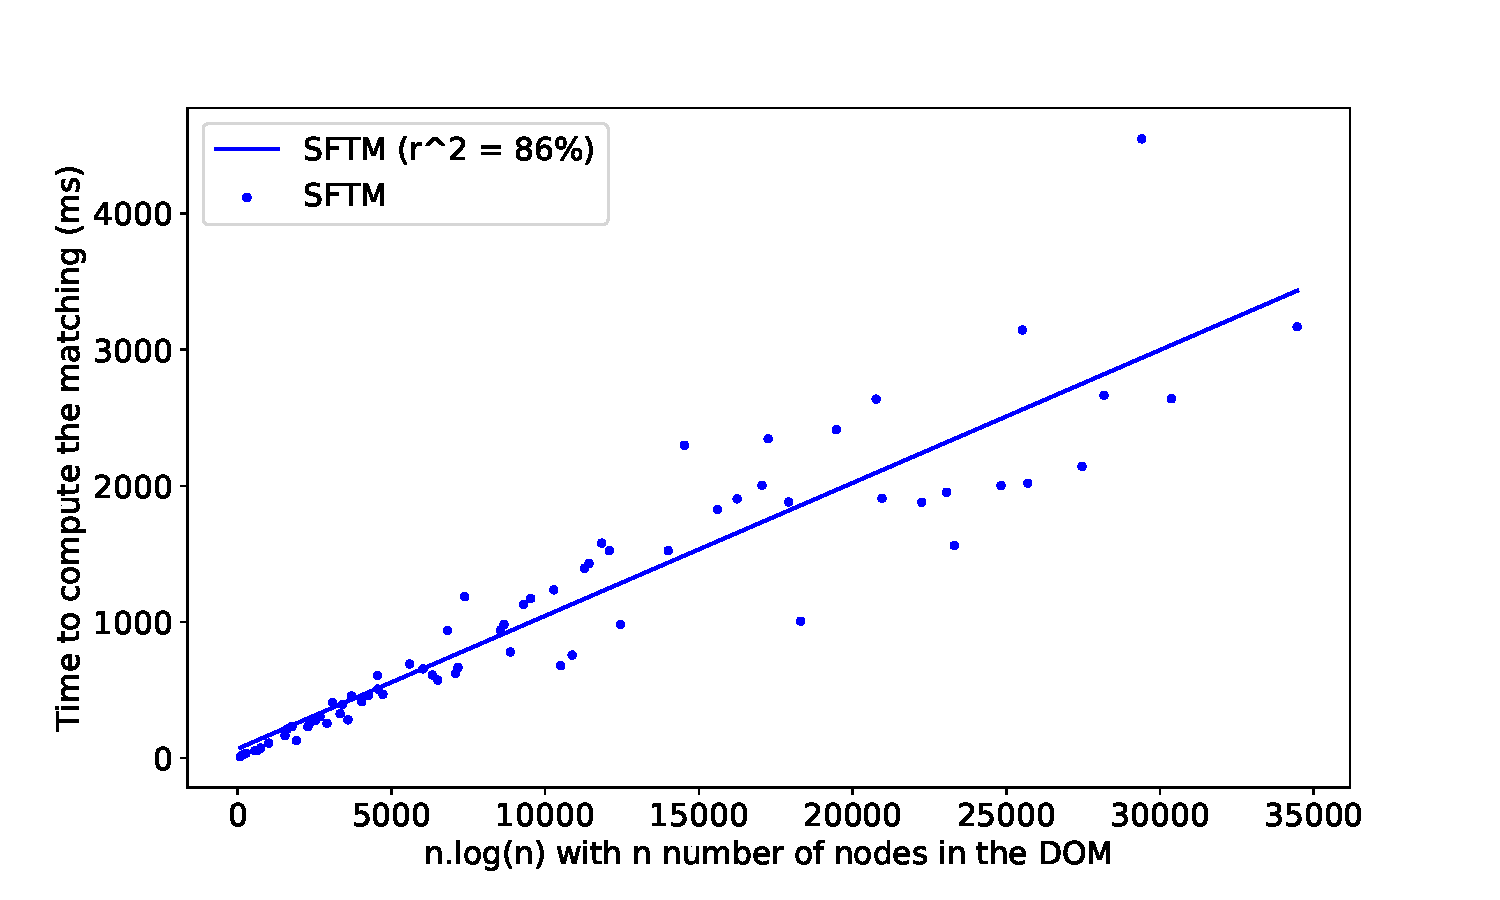
\includegraphics[width=\linewidth]{time_SFTM}
    %     \caption{Average time to compute matching by  $n\ log(n)$ value for SFTM, with $n$ the number of nodes in the DOM}
    %     \label{fig:sftm_speed}
    % \end{figure}
    
% This observation raises the question of the impact of the sublinear threshold function $f$ on the performance of SFTM.
% We therefore conducted a sensitivity analysis of this parameter to better understand potential trade-offs offered by the definition of this function, with regards to the complexity analysis we performed (cf. Section~\ref{sec:complexity}).

\paragraph{Matching efficiency}
The matching efficiency measures how fast a given solution can produce accurate results.
The efficiency is a way to combine both accuracy and speed metrics into one that can be used to compare all solutions.
In our case, we already showed that SFTM outperforms APTED in both accuracy and computation time.
This efficiency measure is thus particularly interesting to compare SFTM to \textsc{XyDiff}, as SFTM outperforms \textsc{XyDiff} in terms of accuracy, but remains slower when it comes to speed.
To compute this matching efficiency, we consider the same metric as~\cite{oliveira2018efficient}---\emph{i.e.}, the number of good matches produced per millisecond.
Figure~\ref{fig:efficiency} reports on the matching efficiency of all three matching solutions.
One can observe that SFTM produces $7.7$ good matches per millisecond on average, which is far above APTED and \textsc{XyDiff} that produce $3.6$ and $2.4$ good matches per millisecond, respectively. 

\begin{figure}
    \centering
    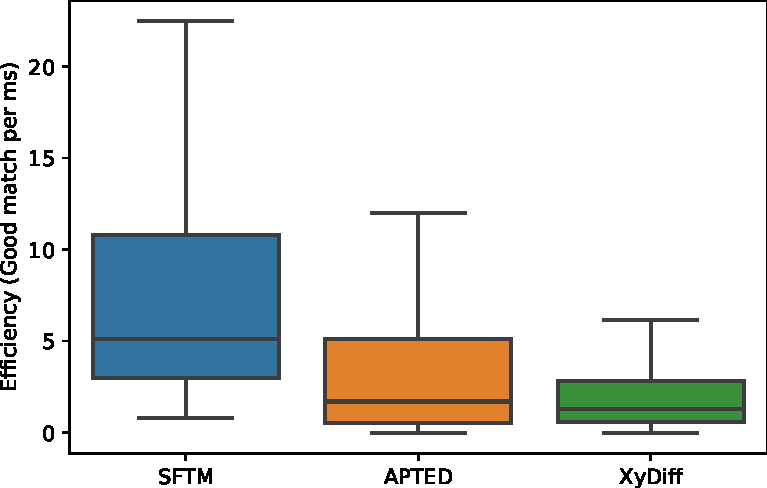
\includegraphics[width=.8\linewidth]{tree-matching/graphs/efficiency}
    \caption{Matching efficiency of SFTM, APTED, and \textsc{XyDiff}.}
    \label{fig:efficiency}
\end{figure}

\paragraph{Parameter sensitivity}
Since we aim at improving the performances of FTM in term of computation times, we study the sensitivity of the sub-linear threshold function $f$, which is a parameter that directly influences the computation time of the algorithm.

Figure~\ref{fig:parameter}, therefore, reports on the evolution of SFTM performances when $f$ varies.
To study the sensitivity of $f$, we choose to use the power function $f(N) = N^\alpha$ as a threshold and display how the computation times and matching accuracy evolve with $\alpha$.

\begin{figure}
    \centering
    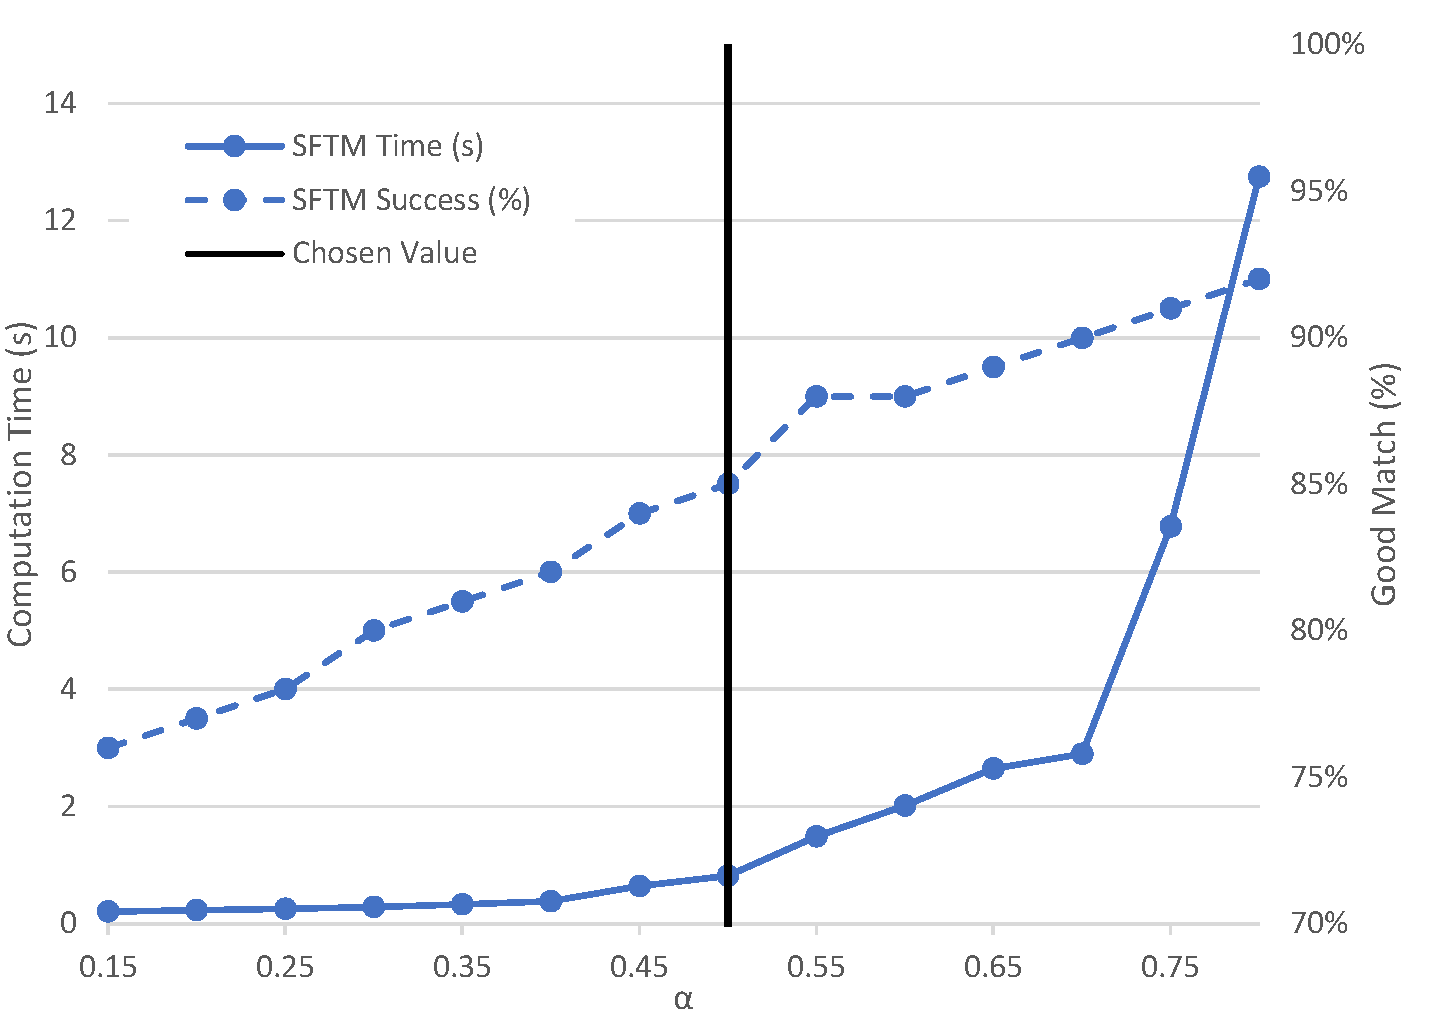
\includegraphics[width=.8\linewidth]{tree-matching/graphs/sensitivity}
    \caption{Performance of SFTM given $f(N) = N^\alpha$ according to $\alpha$.}
    \label{fig:parameter}
\end{figure}

For this experiment, as we are interested in studying the sensitivity of the parameter $\alpha$ on the performances of SFTM, we therefore consider a subset of $243$ pairs from the complete dataset used in previous sections (cf. Section~\ref{sec:performances}), which represents a $6\%$ error margin with $95\%$ confidence.

As expected, when $\alpha$ increases, the quality of the matching and the computation times increase.
However, beyond a certain value of $\alpha$, the increase of computation time is superior to the gain in accuracy: increasing $\alpha$ from $0.5$ to $0.8$ entails more than $10$ times longer computation times for $8\%$ gain in accuracy. 
Intuitively, this is because tokens contained in most nodes provide few relevant information (low IDF), but increase the complexity quadratically.
In this chapter, we thus adopted $\alpha = 0.5$ (\emph{i.e.}, $f(N) = \sqrt{N}$) as this value achieves good enough performances to demonstrate that SFTM can match two real-life web pages in practical time, with a minimum of compromise on quality.  

\section{Threats to Validity}\label{sec:threats}
The absolute values of completion times depend on the machine on which the algorithms were executed.
As computations took time, we had to run both SFTM, APTED and \textsc{XyDiff} on a server, which is shared among several users.
Although we paid a careful attention to isolate our benchmarks, the available resources of the server might have varied along execution thus impacting our results.
% Nevertheless, the repetition of measures reports a clear signal in favour of SFTM.

Our dataset contains the homepages of the Top\,1k Alexa websites.
The fact that our qualitative evaluation has only been conducted on homepages might have biased the results, as such pages might not be fully representative of the complexity of online documents.
Yet, one can observe that the distribution of page sizes in our datasets offers a good diversity of situations.

The parameters used for SFTM and, in particular, the weights for the propagation may not be optimal.
However, our evaluation shows that the adopted values succeed to report tree matchings that compete with the state-of-the-art accuracy in reasonable times and on a very large variety of web pages, which means the values we provided for the parameters do not require to be tuned for most web pages matching cases.

% Finally, our approach consisting in filtering out the tokens contained by more than $f(N) = \sqrt{N}$ nodes is not backed by any theoretical analysis which means we cannot assure the SFTM algorithm with such tuning will conserve the same performance when the number of nodes grows beyond the empirically studied window.

\section{Conclusion \& Perspectives}\label{sec:conclusion}
Comparing modern real-life web pages is a challenge for which traditional \emph{Tree Edit Distance} (TED) and \textsc{XyDiff} solutions are too restricted and computationally expensive. 
\cite{Kumar2011_FTM} introduced \emph{Flexible Tree Matching} (FTM) to offer a restriction-free matching, but at the cost of prohibitive computational times.

This chapter thus introduced \emph{Similarity-based Flexible Tree Matching} (SFTM), the first implementation of an advanced \emph{Flexible Tree Matching} (FTM) algorithm with scalable computation times.
We evaluated our solution using mutations on real-life web pages and we showed that SFTM outperforms \textsc{XyDiff} qualitatively and compares to TED, while significantly improving the computation time of the latter.
Our proof of concept demonstrates that accurate matching of real-life web pages in practical time is possible.

Our \textit{label-centric} approach to matching is significantly different than previous \textit{structure-centric} techniques.
In addition to providing a competitive solution to match web pages, we hope that our solution will encourage the development of solutions based on similar approaches.
We also believe that having a robust algorithm to efficiently compare web pages will open up new perspectives within the web community.

In future work, we will further investigate how to improve the quality of the tree matchings by analyzing which situations cause SFTM to report mismatches and to establish guidelines to adjust the exposed parameters.

Finally, whether our work might be applicable to other trees than web DOMs remains to be demonstrated.
Indeed, SFTM strongly relies on the fact that node labels in DOMs are highly differentiating (many specific attributes on each element), which is not the case for all kinds of trees.

%% TRANSITION
The final objective of our work is to build a set of tools allowing to create an abstraction of any web application. Being able to compare two web pages is a first step.
In the next section, we will apply tree-matching to the robust locator problem.

%% OLD ABANDONNED STUFF

%%e.g: Given an element $E$ to locate,  $P$ is an ancestor of $E$, if $P$ has differentiating attributes (like an \textit{id}) we can locate $E$ relatively to $P$ and identify $P$ using its differentiating attributes. 

%\subsubsection{Stateful identification architecture}
%Existing methods to identify elements on a page (xPath) are limited. Notably, they don't allow to express \textit{flexible}, statistics based identifiers. That's why some works have developed some more flexible identification methods [...] and applied them to repair broken locators.

%If we are capable to use more efficient methods than xPath to identify elements as these studies suggest, why use it only to repair locators and not directly as locators?

%In this contribution, we study the problems that moving to such a flexible identification system might rise and suggest a possible architecture allowing to practically use \textit{stateful identification methods}.

% A naive approach would be to sort all edges by increasing cost and select $min(|U|, |V|)$ edges.
% However, doing so would not guarantee to obtain a full matching, since we might have selected several edges linked to the same nodes.
% A valid approach would rather be to: 
% \begin{compactenum}
%     \item Sort all the edges by increasing cost,
%     \item Select the edge $e$ between $u$ and $v$,
%     \item In the ordered list, remove all edges other than $e$ linked to $u$ and $v$,
%     \item Repeat the selection process (from step (2)) until all edges have been selected/
% \end{compactenum}

% While this approach returns a full matching, it only optimizes the decision one-step-ahead.
% In order to approach the optimal matching, we use the same technique as FTM does: the metropolis algorithm~\cite{metropolis1953equation}.
% The metropolis algorithm provides a way to explore a probability distribution by random walking through samples.
% We use this algorithm to random walk through several full matching, and retain the least costly.
% The algorithm needs to be provided with:
% \begin{compactenum}
%     \item An initial sample $M_0$,
%     \item A suggestion function $suggestMatching: M_t \mapsto M_{t+1}$,
%     \item An objective function we want to maximize: $f(M)$,
%     \item A parameter $N$ that defines the number of random walk to perform before returning the best visited sample.
% \end{compactenum}
% Table~\ref{tab:equivalenceMetropolis} shows the equivalence between the general vocabulary and notations commonly used when describing the metropolis algorithm and our specific application to FTM.

% \begin{table}
% \caption{Equivalence between the Metropolis algorithm and FTM}
% \label{tab:equivalenceMetropolis}
% \begin{tabular}{ll}
% \hline
% Metropolis Algorithm & FTM                                    \\
% \hline
% Sample $x$           & Full matching $M$                      \\
% $Q(x_{t+1}|x_t)$     & $suggestMatching: M_t \mapsto M_{t+1}$ \\
% Probability distribution $P(x)$ & $f: M \mapsto \text{quality of } M)$ \\
% \hline
% \end{tabular}
% \end{table}

\chapter{Erratum}\label{chap:erratum}
\section{Abstract}
% Web applications are constantly evolving to integrate new features or fix reported bugs.
% Such continuous evolutions may alter the content and/or the rendering of web application.
% Underneath, all these web applications relies on the \emph{Document Object Model} (DOM) to render content from web browsers.
% To interact with web applications, \emph{element locators} are identifiers used to navigate across the DOM when automating tasks (\emph{e.g.}. web test scripts, crawlers, or robotic process automation).
% Unfortunately, element locators tend to become fragile when the underlying web pages evolve over time.
% % 
% \emph{Robust locators} have been introduced to overcome this issue, but they fail to repair broken locators on complex and dynamic web applications.
% For this reason, several contributions explored the idea of automatically repairing broken locators on a page. 
% However, these works attempt to repair a given broken locator by scanning all elements in the new DOM to find the most similar one, which fails to scale when the complexity of web pages grows.

Web applications are constantly evolving to integrate new features and fix reported bugs.
% or even simply when the displayed content is updated.
Even an imperceptible change can sometimes entail significant modifications of the \emph{Document Object Model} (DOM), which is the underlying model used by browsers to render all the elements included in a web application.
% In particular, when considering scripts that interact with these web applications (\emph{e.g.} web test scripts, crawlers, or robotic process automation), the continuous evolution of web applications make it extremely challenging to automate the actions on the elements of a web page in a robust way.
Scripts that interact with web applications (\emph{e.g.} web test scripts, crawlers, or robotic process automation) rely on this continuously evolving DOM which means they are often particularly fragile.
More precisely, the major cause of breakages observed in automation scripts are \emph{element locators}, which are identifiers used by automation scripts to navigate across the DOM. When the DOM evolves, these identifiers tend to break, thus causing the related scripts to no longer locate the intended target elements.

% \emph{Robust locators} have been introduced to overcome this issue, but they fail to repair broken locators on complex and dynamic web applications.
For this reason, several contributions explored the idea of automatically repairing broken locators on a page. 
These works attempt to repair a given broken locator by scanning all elements in the new DOM to find the most similar one.
Unfortunately, this approach fails to scale when the complexity of web pages grows, leading either to long computation times or incorrect element repairs.
% 
We therefore, adopt a different perspective on this problem by introducing a new locator repair solution that leverages tree matching algorithms to relocate broken locators.
This solution, named \erratum{}, implements a holistic approach to reduce the element search space, which greatly eases the locator repair task and drastically improves repair accuracy.
% 
We compare the robustness of \erratum{} on a large-scale benchmark composed of realistic and synthetic mutations applied to popular web applications currently deployed in production.
Our empirical results demonstrate that \erratum{} outperforms the accuracy of WATER, a state-of-the-art solution, by 67\%.
% , with no performance penalty.

\section{Introduction}
The implementation of automated tasks on web applications (apps), like crawling or testing, often requires software engineers to locate specific elements in the DOM (\emph{Document Object Model}) of a web page.
To do so, software engineers or automation/testing tools often rely on CSS (\emph{Cascading Style Sheets}) or XPath selectors to query the target elements they need to interact with.
Unfortunately, such statically-defined locators tend to break along time and deployments of new versions of a web application.
This often results in the failure of all the associated automation scripts (including test cases) that apply to the modified web pages.

While several existing works focus on repairing tests on GUI applications, there are surprisingly very few test repair solutions targeting web interfaces~\cite{imtiaz2019systematic}.
These solutions either propose to \emph{i)} generate locators that are robust to changes (so-called \emph{robust locator problem}), or \emph{ii)} repair locators that are broken by the changes applied to the web pages (so-called \emph{locator repair problem}).
Unfortunately, most of the existing solutions in the literature fail to accurately relocate a broken locator, thus leaving all the related web automation scripts as broken~\cite{hammoudi2016record}.
% 
More specifically, state-of-the-art solutions to the locator repair problem, WATER~\cite{choudhary2011water} and VISTA~\cite{stocco2018visual}, tend to rely on the intrinsic properties of the element whose locator needs repairing to locate its matching element on the modified page. 
However, this approach fails to leverage the element position and relations with the rest of the DOM, thus ignoring valuable contextual insights that may greatly help to repair the locator.

We adopt a more holistic approach to the locator repair problem: instead of focusing on the element whose locator is broken individually, we leverage a tree matching algorithm to match all elements between the two DOM versions. 
Intuitively, using a holistic approach to repair a broken locator should significantly improve accuracy by reducing the search space of candidate elements in the new version of the page: for example, if the parent of the element whose locator is broken is easily identifiable (\emph{e.g.}, the item of a menu) a tree matching algorithm will use this information to relocate the target element in the modified page with better accuracy.
Additionally, if more than one locator is broken on a given web page, our approach will repair all of them consistently at once.
The holistic solution we propose, named \erratum{},\footnote{\erratum{} stands for "\erratumlong{}"} more specifically leverages an efficient \emph{Similarity-based Flexible Tree Matching} (SFTM) algorithm to repair all broken locators by matching all changes in a web page with high accuracy, compared to the state-of-the-art solutions.
SFTM is a tree matching algorithm providing fast computation times and high accuracy when compared to other generic tree matching solutions.
To do so, SFTM builds on a distinctive characteristic of DOM trees: the labels of the nodes (\emph{i.e.}, node attributes and tags) contain a high amount of information that can be leveraged to prune the space of possible matchings between two trees.

Evaluating solutions to both robust locator and locator repair problems requires to build a dataset of web page versions---\emph{i.e.}, \textsf{(original page, modified page)} pairs.
Unfortunately, previous works assessed their contributions on hardly-reproducible benchmarks of limited sizes (never beyond a dozen of websites).
We rather evaluate the robustness of our approach against the state of the art by introducing an open benchmark, which covers a wider range of changes that can be found in modern web apps.
Concretely, our open benchmark considers over 83k+ locators on more than $650$ web apps.
It combines \emph{i)} a \emph{synthetic dataset} generated from random mutations applied to popular web apps and \emph{ii)} a \emph{realistic dataset} replaying real mutations observed in web apps from the Alexa~Top\,1K,\footnote{\url{https://www.alexa.com/topsites}} which ranks the most popular websites worldwide.

When evaluated on both datasets, our results demonstrate that \erratum{} outperforms the state-of-the-art solution, namely WATER~\cite{choudhary2011water}, both in accuracy (67\% improvement on average) and performances, when more than 3 locators require to be repaired in a web page.

Concerning the potential applications of \erratum, while we introduce and evaluate our solution within the well-studied context of locator repair, we also discuss a novel resilient architecture centered around \erratum allowing to entirely replace all locator-based interactions.
This architecture intends to support much more interactive and robust script editions in the context of web testing, web crawling, and robotic process automation.

\paragraph{Summary}
Overall, the key contributions in this chapter consist of:
\begin{compactenum}
    \item proposing a solution to the locator repair problem leveraging the principles of \emph{Flexible Tree Matching} (FTM),
    \item implementing and integrating an efficient algorithm, named \erratum, to repair broken locators,
    \item providing a novel, reproducible, large-scale benchmark dataset to evaluate both the robust locator and locator repair problems,
    \item reporting on an empirical evaluation of our approach when solving the locator repair problem,
    \item proposing a novel script edition architecture centered on \erratum.
\end{compactenum}

\paragraph{Outline}
The remainder of this chapter is organized as follows.
Section~\ref{erratum:sec:related-work} introduces the state-of-the-art approaches in the domain of robust locators and locator repair, before highlighting their shortcomings.
Section~\ref{erratum:sec:locator} formalizes the locator problem we address.
Section~\ref{erratum:sec:implementation} introduces our approach, \erratum, which leverages an efficient flexible tree matching solution that we identified.
Section~\ref{erratum:sec:benchmark} describes the locator benchmark we designed and implemented.
Section~\ref{erratum:sec:evaluation} reports on the performance of our approach compared to the state-of-the-art algorithms.
% Section~\ref{erratum:sec:threats} discusses the threats to validity of our contribution.
Finally, Section~\ref{erratum:sec:perspectives} presents some perspectives for this work, while Section~\ref{erratum:sec:conclusion} concludes.

% In order to identify elements on a page, developers usually use CSS Selectors and XPaths...

% These identifiers often break leading to the breakage of the associated tests / robots.
% There are some techniques in the literature to \textit{generate} such \textit{identifiers}, but they are even much more fragile.
% The fragility of automatically generated locators is one of the main obstacles to the development of visual frameworks for test/crawlers development. 
% The problem is such that some articles developed alternative ways to identify elements on a page and used it to repair broken XPath identifiers [.....]
% \subsection{Contribution}\label{erratum:sec:contribution}
% Our contribution is two-fold:
% \subsubsection{Robust locators using tree-matching}
% The expressivity of xPath relies on the ability to use any other elements on the page as anchor to locate another element. 
% This allows to identify elements that do not have intrinsic differentiating features. If we are already using surrounding elements to help in the identification process, why not using \textit{all} other elements?
% In this contribution, we use tree-matching algorithms to match elements of a new version of a page with elements identified in its previous version.
% \subsubsection{Benchmarking tools}
% Existing works on robust locators all evaluate their contribution on a private dataset manually constructed which 
% \begin{enumerate}
% \item Makes it impossible to reproduce
% \item Might be subject to bias (since it was manually constructed) 
% \end{enumerate}
% In order to evaluate the quality of our identification system, we built two datasets, both containing a list of pair $(D, D')$ where $D$ and $D'$ are two different versions of the same page:
% \begin{enumerate}
% \item A synthetic dataset made of different versions of famous websites' pages generated by applying random mutations to the original page
% \item A real world dataset made of different versions in time of the same page, built using the \textit{wayback API} (to retrieve the different versions of the websites)
% \end{enumerate}
% Both datasets are publicly available and the code that generated it is open source.

\section{Background \& Related Work}\label{erratum:sec:related-work}
We deliver a novel contribution to the locator repair problem, which has been initially studied in the domain of web testing.
In this section, we thus introduce the required background and we describe state-of-the-art approaches to repair broken locator, and in particular the literature published in the domain of web test repair.

\subsection{Introducing Web Element Locators}
To detect regressions in web applications, software engineers often rely on automated web-testing solutions to make sure that end-to-end user scenarios keep exhibiting the same behavior along changes applied to the system under test.
% 
Such automated tests usually trigger interactions as sequences of actions applied on selected elements and followed by assertions on the updated state of the web page.
For example, \emph{"click on button $e_1$, and assert that the text block $e_2$ contains the text '{\tt Form sent}'"}.
To develop such test scenarios, a software engineer can
\begin{inparaenum}
    \item manually write web test scripts to interact with the application, or
    \item use record/replay tools~\cite{burg2013interactive,sen2013jalangi,mickens2010mugshot} to visually record their scenarios.
\end{inparaenum}
In both cases, the scenario requires to identify the target elements on the page [$e_1$, $e_2$] in a deterministic way, which is usually achieved using XPath, a query language for selecting elements from an XML document.
% 
For example, let us consider the following HTML snippet describing a form:

\begin{lstlisting}
<form method="post" action="index.php"> 
    <input type="text"   name="username"/> 
    <input type="submit" value="send"/>
</form> 
\end{lstlisting}

The following XPath snippets describe 3 different queries, which all result in selecting the submit button: \lstinline!/form/input[2]!, \lstinline!/form/input[@value="Send"]!, \lstinline!input[@type="submit"]!.
In the literature, such element queries or identifiers are named \emph{locators}~\cite{leotta2014reducing}.

In practice, automated tests are often subject to breakages~\cite{hammoudi2016record}.
It is important to understand that a test \textit{breakage} is different from a test \textit{failure}~\cite{stocco2018visual}: a test failure successfully exposes a regression of the application, while a test is said to be broken whenever it can no longer apply to the application (\emph{e.g.}, the test triggered a click on a button $e$, but $e$ has been removed from the page).
While there can be many causes to test breakage, \cite{hammoudi2016record} reports that $74\,\%$ of web tests break because one of the included locators fails to locate an element in a web page.

% While we focus on web test repair, some previous work focused on GUI test repair for desktop applications~\cite{grechanik2009maintaining,zhang2013automatically,memon2008automatically,gao2015sitar,daniel2011reassert}.
% This work most often uses platform-specific features hardly transposable to the web, as Zhang~\emph{et~al.}~\cite{zhang2013automatically} who rely on the methods associated to GUI elements.

\subsection{Generating Web Element Locators}\label{erratum:sec:sota_robust_locator}
The fragility of locators remains the root cause of test breakage, no matter
they have been automatically generated (\emph{e.g.}, in the case of
record/replay tools), or manually written. To tackle this limitation, several
studies have focused on generating more robust locators. This includes
ROBULA~\cite{leotta2014reducing}, ROBULA+~\cite{leotta2016robula+}, which are algorithms that apply successive refining transformations from a raw XPath query until it yields an xPath locator that exclusively returns the desired element. Leotta~\emph{et~al.}~\cite{leotta2015meta,leotta2021sidereal} also propose
Sideral, a graph-based algorithm to generate xPath locators. Sideral requires to
specifically train on each application in order to learn what properties are
most likely safe to rely on when building xPath locators. While these methods
all use ancestors of a given elements as anchor to generate a locator,
\cite{nguyen2021generating} uses siblings instead, arguing that they make more
reliable anchors.

Another work by Yandrapally~\emph{et~al.} leveraged
contextual clues to generate locators~\cite{yandrapally2014robust}. These clues
rely mostly on the content surrounding the element to locate which may be
problematic in case the content changes. LED~\cite{bajaj2015synthesizing} uses a
SAT solver to select several elements at once, but is never evaluated on
different DOM versions. Finally, some works combine several locator generators
with a voting mechanism to locate a single element with more
robustness~\cite{leotta2015using, zheng2018method, long2020webrr}. However, all
these approaches, which consider a limited set of locator generators, strongly
depend on the accuracy of individual algorithms to agree upon a single and
relevant locator.

While automatically generating locators can speed up the
definition of test cases, it becomes a keystone for visually-generated test
cases based on record/replay tools. In the end, the reliability of test cases
built using such a tool depends mostly on the quality of the locators it
automatically generates~\cite{hammoudi2016record}.

% \vspace{6pt}\noindent\textbf{Challenge.}
% We formalize this challenge of generating more robust locators as the \emph{robust locator problem} (cf. RQ.~\ref{robust_locator_problem} for a more formal definition).

\subsection{Repairing Web Element Locators}
While some solutions to the robust locator problem, as presented above, aim to prevent locators from breaking, others focus on repairing broken locators.
In this context, the repair tool considers
\begin{inparaenum}[\em a)]
    \item the descriptor of the locator,
    \item the last version of the page on which the locator was still functional ($D$),
    \item the new version of the page on which the locator is broken ($D'$).
\end{inparaenum}

\paragraph{Property Based}
In this area, WATER~\cite{choudhary2011water} and COLOR~\cite{kirinuki2019color}
provide algorithm to fix broken tests using intrinsic properties of the element
to relocate.
The process of repairing a test involves several steps: 
\begin{inparaenum}
\item running the test, 
\item extracting the causes of failure and,
\item repairing the locator, if broken. 
\end{inparaenum}
The last part is particularly challenging. 
To relocate a locator from one version to another, WATER and COLOR scan all elements in the new version and return the most similar one to the element in the original version with regards to intrinsic properties (\emph{e.g.}, absolute XPath, classes, tag).
Hammoudi~\emph{et~al.}~\cite{hammoudi2016waterfall} further studied the locator repair part of WATER and found that repairing tests over finer-grained sequences of change (typically commits) contributes to improving accuracy.

\paragraph{Vision Based}
Using a completely different approach, VISTA~\cite{stocco2018visual} is a recent technique that adopts computer vision to repair locators. VISTA falls within the category of computer vision-aided web tests~\cite{chang2010gui,leotta2018pesto,alegroth2013jautomate}.
However, while using computer vision succeeds in repairing most of the \textit{invisible} changes, such solutions tend to fail when the content, the language, or the visual rendering of the website changes.
Furthermore, visual-based solutions fail to locate dynamic elements that only appear through user interactions (\emph{e.g.}, a dropdown menu).

Finally, J.Imtiaz et al~\cite{imtiaz2021automated} developed a test repair
solution that integrates to several different capture replay tools. While we
focus specifically on the locator repair problem, they used and evaluated a more
comprehensive test-repair strategy involving the classification of the test script and
detected breakages and the extension of the UML Testing Profile specifications to
capture more interaction details.

% \vspace{6pt}\noindent\textbf{Challenge.}
% The challenge of any locator repair solution is therefore to successfully locate any element(s) selected by the locator on the original page, on the new page.
% This is what we call the \emph{locator repair problem} (cf. Section~\ref{locator_repair_problem} for a more formal definition).

\begin{figure*}
    \centering
    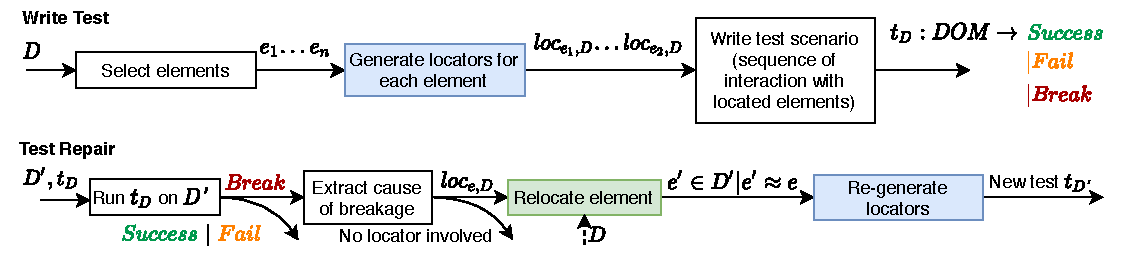
\includegraphics[width=1\linewidth]{erratum/locator-repair}
    \caption{Illustration of the locator problem statement in automated tests combining the \emph{robust~locator}~(in~blue) and the \emph{locator~repair}~(in~green)~problems.}
    \label{fig:locator_repair}
\end{figure*} 

% =============================== PROBLEM STATEMENT =================================
\section{Locator Problem Statement}\label{erratum:sec:locator}
Figure~\ref{fig:locator_repair} summarizes the steps to follow when writing or repairing a locator in a web test script.
When a test breaks, the repairing process generally includes three main steps: 
\begin{inparaenum}
    \item extract the cause of the breakage
    \item if a locator caused the breakage, the element is first relocated then
    \item a new locator is generated/written.
\end{inparaenum}
Beyond automated tests, this problem can also arise in more general web automation scripts covering web content crawling and \emph{Robotic Process Automation} (RPA), which heavily rely on locators to automate the navigation across web applications.

In this section, we formalize the description of two locator-related problems highlighted in Figure~\ref{fig:locator_repair}, namely the \emph{robust locator} (in blue) and \emph{locator repair} (in green) problems for the general case of web automation scripts.

\subsection{Problem Notations}
We consider that a given web page can change for various reasons, such as
\begin{inparaenum}
    \item content variation,
    \item page rendered for different regions/languages, or
    \item release of the web application.
\end{inparaenum}
No matter the cause, we distinguish $D$ and $D'$ as two versions of the same web page observed before and after a change, respectively.
More specifically, we define the following similarity notations:
\begin{compactenum}
\label{def:similarity}
    \item $D \approx D'$ if scripts written for $D$ are expected to apply on $D'$;
    \item Given 2 web elements $e \in D$ and $e' \in D'$, $e \approx e'$ if $e$ and $e'$ refer to semantically equivalent elements (\emph{e.g.}, the same menu item observed in pages $D$ and $D'$);
    \item By extension of (2), given a set of elements $E = {e_1...e_n} \subset D$ and $E' = {e'_1...e'_{n'}} \subset D'$, $E \approx E'$ if $n = n'$ and, for each $i \in [1..n]$, $e_i \approx e'_i$.
\end{compactenum}

% The above similarity definitions rely on the semantics of a web page and its embedded elements. 
% However, whether two elements or pages, share the same semantics might be hard to decide.
% The subjective part of this similarity measure is, however, difficult to avoid since we aim to capture the similarity as perceived by a developer.
% We discuss more concrete examples in Section~\cite{erratum:sec:XXX}.

Based on the above similarity notation, we provide the following definitions:
\begin{defn}\label{loc_def}
    Given a page $D$, and a set of elements $E = {e_1...e_n}$, the pair $(loc_{E,D}, eval)$ is a \textbf{locator} of $E$ with regard to $D$ if:
    \begin{equation}
       eval(loc_{E,D}, D) = E
    \end{equation}
    where $loc_{E,D}$ is a descriptor of $E$ and $eval$ an evaluation function that returns a set of web elements from a descriptor and an evaluation context (\emph{e.g.}, a web page).
\end{defn}
In the case of XPath-based locators, the descriptor $loc_{E,D}$ refers to an XPath query describing the elements $E$ in the page $D$ and $eval$ the XPath solver.

\begin{defn}
    Let $mut$ be a mutation function that transforms the page $D$ into another page $D'$, such as $mut(D) = D'$.
    $mut$ is said to be a \textbf{mutation} of $D$ if $D \approx D'$.
\end{defn}

\begin{defn}
    Given a locator $L = (loc_{E,D}, eval)$, $L$ is \textbf{robust} to a mutation function $mut$ if:
    \begin{equation}
       eval(loc_{E, D}, mut(D)) \approx E
    \end{equation}
\end{defn}

Finally, we note $\lambda(e)$ the label of the node $e$ in the DOM tree. The label of a node comprises the tag, the attributes and their values and the textual content. However, in the context of \erratum, we willingly ignore the content as described in section \ref{erratum:sec:node_similarity}.

\subsection{Problem Statement}
Given the above definitions, we can formalize the locator problem statement along with the two following research questions.
\begin{rqn}\label{robust_locator_problem} % Not sure we can label it as "RQ"
    \textbf{Robust Locator}. 
    For any subset of elements on a given page $D$, how to automatically generate locators that are robust to mutations of $D$?
\end{rqn}
When evaluating a locator on a new page $D'$, the only available information to describe the targeted element is the descriptor $loc_{E,D}$, which often remains insufficient (cf. state-of-the-art techniques).

On the other hand, in the context of \textit{locator repair}, the original page $D$ from which $loc_{E,D}$ was built is available.
Thus, using definition~\ref{loc_def}, this piece of information allows to locate the originally selected elements $eval(loc_{E,D}, D) = E$.

\begin{rqn}\label{locator_repair_problem}
    \textbf{Locator Repair}. 
    Given two pages $D$, $D'$, such that $D \approx D'$ and a set of elements $E\in D$, how to locate the elements $E' \approx E$ in $D'$?
\end{rqn}
To the best of our knowledge, existing solutions to both \emph{robust locator} and \emph{locator repair} focus on the restricted case of $|E| = 1$.
% We call such locators---\emph{i.e.}, $\{l = (loc_{E,D}, eval) \text{ where }|E| = 1\}$---\textit{single-element locators}.

Once the \textit{locator repair problem} is solved (\emph{i.e.}, $E'$ are correctly located), we need to generate new locators, which brings us back to the situation of the robust locator problem (cf. RQ.~\ref{robust_locator_problem}).

We thus present a novel approach to solve the locator repair problem.


% =================================== ERRATUM ========================================
\section{Repairing Locators with \erratum}\label{erratum:sec:implementation}
% \subsection{Overview}
The previous section formalized both \emph{robust locator} and \emph{locator repair} problems.
% In a browser, HTML web pages are parsed into a \emph{Document Object Model} (DOM), which is a labeled tree where most nodes are elements embedded in the web page.
% Existing approaches to locate web elements in such a DOM tree consider the locator to repair individually and generally build on the structure of the tree (XPath~\cite{leotta2016robula+}, CSS selectors), on fuzzy matching of elements' properties (WATER~\cite{choudhary2011water,hammoudi2016waterfall}), on contextual clues~\cite{yandrapally2014robust} or on the visual appearance of elements (VISTA~\cite{stocco2018visual}) to repair one specific locator.
The approach we report, \erratum, therefore matches the DOM trees of 2 versions of a web page to solve the \emph{locator repair} problem.
Several tree matching solutions exist in the literature, such as \emph{Tree Edit Distance} (TED)~\cite{tai1979tree} or tree alignment~\cite{jiang1994alignment}.
This section therefore motivates and explains how \erratum leverages tree matching to repair locators, before discussing the choice of a tree matching implementation fitting \erratum's requirements.

\subsection{Applying Tree~Matching to Locator~Repair}
Embedding tree matching allows \erratum to leverage the tree structure in the same way an XPath-based solution would, while offering the flexibility of a more statistic-based solution.
Intuitively, a tree matching algorithm should consider all easily identifiable elements on a page (elements with rare tags, unique classes, ids, or other attributes) as \textit{anchors} to relocate less easily identifiable elements.

Figure~\ref{fig:holistic} illustrates the benefits of a more holistic approach using tree matching.
In the example, the locator of element \texttt{a} (in blue) breaks because the mutations between $D$ and $D'$ entails a change in its absolute XPath (\texttt{/body/div/a}).
Attempting to repair such a broken locator by relying on the properties of the original element alone (state-of-the-art approaches like~\cite{choudhary2011water,stocco2018visual}) is often challenging and can easily lead to a mismatch. 
% Therefore, we privilege a more holistic approach based on tree matching.
By using tree matching (cf. right-bottom of Figure~\ref{fig:holistic}), matching the parent of the element to locate (\textsf{div\#menu}) brings instead a strong contextual clue to accurately relocate the element \texttt{a$_1$'} whose locator was broken~\ref{chap:sftm}.

\begin{figure}[]
    \centering
    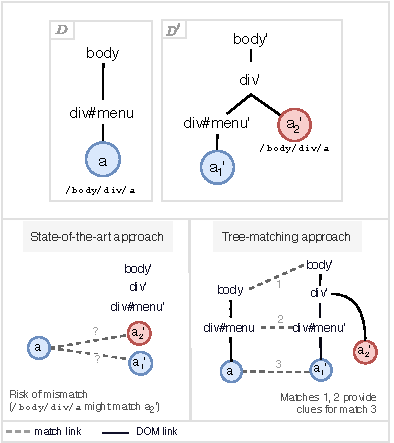
\includegraphics[width=.8\linewidth]{erratum/holistic}
    \caption{State-of-the-art Vs. tree matching locator repair.}
    \label{fig:holistic}
\end{figure}

Formally, given a pair of page versions $D$ and $D'$, we:
\begin{compactenum}
    \item parse $D$ and $D'$ into DOM trees $T$ and $T'$.
    Consequently, $nodes(T)$ is the set of elements in the DOM tree $T$;
    \item apply tree matching to $T, T'$ yielding a matching $M \subset nodes(T) \times nodes(T')$.
    If the resulting matching $M$ is accurate, then $\forall (e, e') \in M, e \approx e'$;
    \item use the resulting matching $M$ to repair the broken locator(s).
\end{compactenum}

Regarding the test repair process illustrated in Figure~\ref{fig:locator_repair}, our approach thus fits in the block "\textsf{relocate element}" (in green) by matching the elements of $D$ in $D'$ and reporting the relocated element. 
Thus, once the element is relocated using tree matching---\emph{i.e.} \erratum found $e' \in D'|e \approx e'$---we only need to generate a new locator $loc_{e', D'}$ to achieve the test repair process.
This task can be performed using solutions to the robust locator problem, like ROBULA~\cite{leotta2014reducing}, and is therefore considered as out of the scope of our study.

\subsection{Integrating a Scalable Tree Matching Algorithm}
The state-of-the-art approach to match two trees is \emph{Tree Edit Distance} (TED)~\cite{tai1979tree}. 
When comparing two trees $T$ and $T'$, TED-based approaches rely on finding the optimal sequence of relabels, insertions and deletions that transforms $T$ into $T'$.
Unfortunately, TED might be unsuitable to match real-life web pages due to two core restrictions~\cite{Kumar2011_FTM}:
\begin{inparaenum}
    \item if two nodes $e$ and $e'$ are matched, the descendants of $e$ can only match with the descendants of $e'$, and
    \item the order of siblings must be preserved.
\end{inparaenum}
Furthermore, TED is computationally expensive ($O(n^3)$ for the worst-case complexity~\cite{bringmann2018tree}) and, more practically, our preliminary experimentation has shown that applying the state-of-the-art implementation of TED, named APTED~\cite{pawlik2016tree}, on the \textit{YouTube} page takes several minutes. 
We believe that, in addition to qualitative restrictions, such computation times are not acceptable when periodically repairing locators on real websites.

Further studies of TED proposed to improve computation times~\cite{jiang1995alignment, valiente2001efficient, zhang1996constrained}, but at the cost of even more restrictive constraints on the produced matching (\emph{e.g.}, the tree alignment problem~\cite{jiang1995alignment} restricts the problem to transformations where insertions are performed before deletions).

To the best of our knowledge, the only contribution that provides a solution to the general (restriction-free) tree-matching problem is the \emph{Flexible Tree Matching} (FTM) algorithm~\cite{Kumar2011_FTM}.
FTM models tree matching as an optimization problem: given two trees $T$ and $T'$ how to build a set of pairs $(e,e') \in T \times T'$ such that the similarity between all selected node pairs is maximal.
The similarity used by FTM combines both the labels and the topology of the tree.

However, as shown in~\ref{chap:sftm}, the theoretical complexity of FTM is high ($O(n^4)$) and the implementation of FTM was shown to take more than an hour to match a web page made of only 58 nodes, while the average number of nodes on a web page observed in our dataset is $1,507$.
Consequently, we believe that such computation times make FTM unpractical in the context of locator repair.

% Given the above review, we therefore integrate SFTM as the reference tree matching algorithm implementation to relocate elements in \erratum and, in the following sections, we evaluate its effectiveness to repair broken locators in web test scripts.

\subsection{Matching DOM Trees by Similarity}\label{erratum:sec:SFTM}
Given the limitation of FTM, \erratum{} integrates a \emph{Similarity-based Flexible Tree Matching} (SFTM) algorithm, which is an extension of state-of-the-art FTM to improve the computation times of FTM without any restriction on the resulting matching~\ref{chap:sftm}. 

In the context of \erratum{}, the SFTM algorithm assumes that, given a web page, several elements are easily identifiable by considering their intrinsic properties.
The algorithm first assigns scores to all possible matches between nodes from the two trees based on their label and only then uses the topology of the trees to adjust these scores.

Almost all existing tree matching algorithms rely first and foremost on the topology of the trees.
Conversely, SFTM relies mostly on the labels of the trees and only makes use of topology in a second step, to fine-tune the already computed scores. Intuitively, matching two sets of labels is significantly easier than trying to match trees, which is the reason why SFTM achieves such competitive performances.
The only trade-off of this approach is that it requires the labels of the trees to be highly differentiating (\emph{i.e.}, carry a lot of information). 
Fortunately, this is the case for the great majority of web pages.

We walk through the key steps of the SFTM algorithm we integrated in \erratum{} by using HTML snippets reported in Figure~\ref{fig:example_html}.
The figure provides two versions ($D$ and $D'$) of a simplified HTML code sample extracted from the homepage of the famous search engine \textit{duckduckgo.com}.
In this example, our purpose is to relocate $\text{a}_1 \in D$ with $\text{a}_1' \in D'$.

% \begin{figure}
%   \centering
%   \begin{subfigure}[b]{0.5\linewidth}
%   \centering
%     \begin{lstlisting}[]
%     for i:=maxint to 0 do
%     begin
%     { do nothing }
%     end;
%     \end{lstlisting}
%     \caption{A listing}
%   \end{subfigure}
%   \hfill
%   \begin{subfigure}[b]{0.5\linewidth}
%     \centering
%     \rule{1.5cm}{1.5cm}
%     \caption{A diagram}
%   \end{subfigure}
%   \caption{A listing and a diagram}
% \end{figure}
\begin{figure}
    \centering
    \begin{subfigure}[b]{\linewidth}
        \centering
        \caption{Original document $D$.}
        \begin{lstlisting}[language=html, label={fig:first_version}]
<div class="content-info__item"> /*!\mymk{div_1}!*/
    <div class="item__title">...</div> /*!\mymk{div_2}!*/
    <div class="item__subtitle"> /*!\mymk{div_3}!*/
        ... 
        <a href="/plugins">Plugins</a> /*!\mymk{~a_1~}!*/
    </div>
</div>
        \end{lstlisting}
    \end{subfigure}
    \hfill
    \begin{subfigure}[b]{\linewidth}
        \centering
        \caption{Updated document $D'$ from $D$.}
        \begin{lstlisting}[language=html, label={fig:second_version}]
<div class="items-wrap"> /*!\mymk{div'_4}!*/
    <div class="item"> /*!\mymk{div'_1}!*/
    <div class="item__title">...</div> /*!\mymk{div'_2}!*/
        <div class="item__subtitle"> /*!\mymk{div'_3}!*/
            ... 
            <a href="/extensions">Extensions</a> /*!\mymk{~a'_1~}!*/
        </div>
    </div>
    <div> /*!\mymk{div'_5}!*/  
        ...
        <a href="/newsletter">Newsletter</a> /*!\mymk{~a'_2~}!*/
    </div>
</div>
        \end{lstlisting}
    \end{subfigure}
    \caption{Two versions of an HTML snippet extracted from the homepage of \emph{duckduckgo.com}.}
    \label{fig:example_html}
\end{figure}

Unlike the state-of-the-art matching algorithms, SFTM first tries to match elements in $D'$ whose labels are similar to $D$, before using these matched elements to adjust the similarity of surrounding elements in the tree.
For example, the \emph{similarity scores} of the tuple $(a_1,a'_1)$ links will increase as their direct parents $(div_3,div'_3)$ are matched with confidence.
% 
Figure~\ref{fig:steps_sftm} summarizes the SFTM algorithm's key steps and the remainder of this section provides an overview of its integration in \erratum{} (cf. green box in Figure~\ref{fig:locator_repair}).
The interested reader can refer to our technical report~\ref{chap:sftm} for an exhaustive description of our SFTM algorithm, whose applications go beyond the context of repairing broken locators.

\paragraph{Step\,1: Node Similarity}\label{erratum:sec:node_similarity}
Elements of DOMs $D$ and $D'$ are compared. 
The first step consists in computing an \emph{initial similarity} $s_0 : D \times D' \to [0, 1]$.
For each pair of nodes $(e, e') \in D \times D'$, $s_0(e,e')$ measures how similar the labels of $e$ and $e'$ are.
In HTML pages, the label of a node $e \in D$ that we use is the set of tokens obtained from applying a tokenizer to the HTML code describing $e$. 
This may include the type of the HTML element, its attributes, and eventually the raw content associated to this element---\emph{i.e.}, thus ignoring the content from the child elements.
% After empirically comparing different settings, we noticed that the algorithm performed better (and faster) when ignoring the content of the elements thus only using the tag name and attributes.
% For example, the label of $div_1$ is the following set of tokens $\{\text{div}, \text{class}, \text{content-info__item} \}$
\begin{ex}
The \emph{label} computed for $div_1$ (cf. Figure~\ref{fig:example_html}) includes the following tokens: $\{\texttt{div}, \texttt{class}, \texttt{content-info\_\_item} \}$. %The algorithm ignores the content.
\end{ex}
% For example, the label of $div_1$ is the following set of tokens $\{\text{div}, \text{class}, \text{content-info\_\_item} \}$

To compute $s_0$, SFTM first indexes the labels of each node of $D$.
The idea of this step is to prune the space of possible matches by pre-matching nodes with similar labels.
When indexing, to improve the accuracy of $s_0$, we apply the \emph{Term Frequency-Inverse Document Frequency} (TF-IDF)~\cite{jones1972statistical} formula to take into account how rare each token is.
\begin{ex}
    Following our previous Example~\ref{fig:example_html}, when considering the match $(div_1, div'_1)$:
    \begin{compactenum}
        \item token $\texttt{div}$ will yield very few similarity points, since it is included in the labels of almost all the nodes,
        \item token $\texttt{content-info\_\_item}$ will increase the score significantly, as it only appears once in both documents.
    \end{compactenum}
\end{ex}
% Following our previous example~\ref{fig:example_html}, when considering the match $(div_1, div'_1)$:
% \begin{compactenum}
% \item the token $\text{div}$ that both elements have in common will yield very few similarity points since it appears in the labels of almost all nodes.
% \item The token $\text{content-info\_\_item}$ will increase the score significantly as it only appears once in both documents.
% \end{compactenum}

In general, very common tokens bring very few information to the relevance of a given match, while they cause a significant increase of potential matches to consider.
That is why, in order to reduce the computation times, the algorithm rules out most common tokens.

\paragraph{Step\,2: Similarity Propagation}
The initial similarity $s_0$ only takes into account the labels of nodes.
In this second step, the idea is to enrich the information contained in $s_0$ by leveraging the topology of the trees $D$ and $D'$.
\begin{ex}
    In Example~\ref{fig:example_html}, it is hard to choose the correct match $m_1 = (a_1, a'_1)$ over the incorrect one $m_2 = (a_1, a'_2)$ by only considering labels, since all three elements share the same set of tokens: $\{\texttt{a}, \texttt{href}\}$.
    In the similarity propagation step, we leverage the fact that the parents of $a_1$ and $a'_1$ are similar to increase the similarity between $a_1$ and $a'_1$, thus preferring $m_1$ over $m_2$.
\end{ex}
% In our example~\ref{fig:example_html}, it is hard to choose the correct match $m_1 = (a_1, a'_1)$ over the incorrect one $m_2 = (a_1, a'_2)$ using only labels since all three elements have the same set of tokens in common: $\{\text{a}, \text{href}\}$. In the similarity propagation step, we use the fact that the parents of $a_1$ and $a'_1$ are similar to increase the similarity between $a_1$ and $a'_1$ which allows to successfully choose $m_1$ over $m_2$.
In general, for each considered match $(e, e') \in D \times D'$, the parents of $e$ and $e'$ gets more similarity points if $e$ and $e'$ are similar and inversely, $s(e, e')$ is increased if the parents of $e$ and $e'$ are similar (with regard to $s_0$).
We call $s$ the final similarity produced by this step.

\paragraph{Step\,3: Optimization}
Producing the optimal matching with regards to the computed similarity means selecting the full set of matches such that each element of $D$ is matched with at most one element of $D'$ and the sum of similarity scores of the selected matches is maximum.

In order to approximate the optimal set of matches, SFTM implements the Metropolis algorithm~\cite{metropolis1953equation}.
The idea is to randomly walk through several possible configurations (set of matches) to converge towards the optimal one.

\begin{figure*}[!t]
    \centering
    \includegraphics[width=\linewidth]{erratum/explanations/sftm}
    \caption{Key steps followed by our \emph{Similarity-based Flexible Tree Matching} (SFTM) algorithm.}
    \label{fig:steps_sftm}
\end{figure*}

At the end of the optimization step, the SFTM algorithm yields a full matching $M \subset D \times D' $ comprising matches between nodes of $D$ and $D'$.
These matches can be analyzed by \erratum{} to locate broken locators and fix them by generating new locators in the target document $D'$.

\paragraph{Best and worst case scenarios}
The greatest strength of \erratum's approach is to handle variations of labels---\emph{e.g.}, renaming a class, adding an id, removing an attribute.
This is because of the fuzzy nature of the first similarity steps of SFTM: as
long as two elements' label share enough rare tokens, they will match.
For elements that have few information in their label (\emph{e.g.}, a bare $div$ tag with no attributes) the algorithm will still be able to rely on the parents and children of the node whose label may contain more discriminative information.

The worst case scenario happens when making structural changes around nodes with with labels containing few information.
For example, if the content of a bare $div$ node is moved to another $div$ node,
matching the first $div$ node accurately will become very challenging.
More than that, since the node that was moved contains high amount of information, the matching of this node will propagate to its new parents, thus increasing the chances of mismatch in the surrounding of the moved node.

% In the rest of the article, we integrate SFTM as the reference flexible tree matching algorithm in \erratum{} to repair broken locators (cf. green box in Figure~\ref{fig:locator_repair}).

% ================================= BENCHMARK ===================================
\section{The Robust Locator Benchmark}\label{erratum:sec:benchmark}
In our context we are interested in covering the following research questions:
\begin{rqn}\label{rq:performance}
    How does \erratum{} perform in solving the locator repair problem (cf. RQ.~\ref{locator_repair_problem}) when compared to state-of-the-art solutions?
\end{rqn}
\begin{rqn}\label{rq:influenceFactors}
    What are the factors influencing the accuracy of WATER and \erratum?
\end{rqn}
\begin{rqn}\label{rq:computationTime}
    How quickly can \erratum{} repair broken locators when compared to state-of-the-art solutions?
\end{rqn}
This section, therefore, describes the benchmark we propose to assess these questions.

\subsection{Evaluated Locator Repair Solutions}\label{erratum:sec:consideredSolutions}
We compare two solutions: 
\begin{inparaenum}
    \item \erratum{}, our approach to repair broken locators by leveraging flexible tree matching, and
    \item WATER, the reference implementation of a locator repair technique applied to web test scripts~\cite{choudhary2011water}.
\end{inparaenum}

% WATER was designed to repair web test cases.
The original algorithm of WATER analyses a given test case, finds the origin of the test breakage, and suggests potential repairs to the developer.
In our context we are interested in the most challenging part of the algorithm: the part that repairs broken locators, if needed.
Given the originally located element $e \in D$, WATER attempts to find $e' \in D'$ such that $e' \approx e$ by scanning over all elements in $D'$ such that $tag(e') = tag(e)$ and selecting the elements most similar to $e$. 
The similarity between two elements $e_1, e_2$ used by WATER mostly consists in computing the Levenshtein distance between the absolute XPaths of both elements ($Levenshtein(XPath(e_1), XPath(e_2))$) combined with other element properties similarity (\emph{e.g.}, visibility, z-index, coordinates).
In our evaluation, we re-implemented this part of the WATER algorithm to compare its performance to \erratum{}.

We initially considered VISTA~\cite{stocco2018visual} as a baseline, even though the approach they use (computer vision) is radically different from \erratum{} and WATER.
However, despite our efforts, we failed to run their implementation and received no answer when trying to contact the authors. 

Note that, in this evaluation, we focus on \textit{single-element locator} cases of the locator repair problem (we only try to repair \textit{single-element locators}).
The reasons for this decision are:
\begin{inparaenum}
    \item The state-of-the-art solutions to both repair and robust locator problems only treat this case and in particular, WATER can only repair locators locating a single element,
    \item \erratum{} reasons on the whole trees, so locating several independent elements is done the same way as locating a group of elements.
\end{inparaenum}

\subsection{Versioned Web Pages Datasets}
In the remainder of this chapter, we propose two datasets to compare \erratum{} and WATER against potential evolutions of web pages.
Given two versions of the same page $D, D'$, and a set of elements $E \subset D$, the locator repair problem consists in locating a set of elements $E' \subset D'$, such that $E' \approx E$.
To evaluate the performance of a locator repair tool, we thus need what we call a \textbf{DOM versions dataset}: a dataset of pairs $(D, D')$, such that $D \approx D'$.

A DOM version dataset is also required to evaluate solutions to the robust locator problem.
To build such a dataset, previous works on locator repair~\cite{leotta2016robula+,leotta2014reducing} and robust locator~\cite{stocco2018visual,choudhary2011water,hammoudi2016waterfall} manually analyzed different versions of a few open source applications (like Claroline, AddressBook or Joomla).
These evaluations are significantly limited in size (never beyond a dozen of websites considered) and hard to reproduce since the exact versions of the open source applications used are often not provided or available.

In our study, we therefore introduce the first large-scale, reproducible, real-life \textit{DOM versions dataset} that can be used to assess locator repair solutions, and is composed of two parts:
\begin{compactenum}
    \item A {\bf \textsc{Mutation} dataset}~\ref{chap:sftm} generated by applying random mutations to a given set of web pages (see Section~\ref{mutationDataset}),
    \item A {\bf \textsc{Wayback} dataset} collects past versions of popular websites from the Wayback API (see Section~\ref{waybackDataset}).
\end{compactenum}

Then, for each pair $(D, D')$ in the dataset, our experiments consist of selecting a set of elements to locate in $D$ and in comparing both \erratum{} and WATER trying to find the corresponding element on $D'$.
% We ran the simulations on both datasets at the same scale in order to avoid potential evaluation bias. 

Table~\ref{table:describing_datasets} describes both datasets in terms of:
\begin{compactenum}
    \item \textbf{\# Unique URLs}: the number of unique URLs among the total of version pairs in the dataset. The duplication is due to the fact that there can be several mutations or successive versions of the same web page. In the case of the {\sc Wayback} dataset, more popular websites are more represented (see Section~\ref{waybackDataset});
    \item \textbf{\# Version pairs}: the number of considered pairs of web pages $(D, D')$,
    \item \textbf{\# Located elements}: the number of elements $e \in D$ that any solution should locate in $D'$.
\end{compactenum}

\begin{table}[!htbp]
    \caption{Description of the \textsc{Mutation} \& \textsc{Wayback} datasets.}
    \label{table:describing_datasets}
    \centering
    \resizebox{.6\linewidth}{!}{%
        \begin{tabular}{|l|r|r|}
        \hline
         Dataset      & {\sc Mutation} & {\sc Wayback} \\ \hline
        \hline
        \# Unique URLs      &      650 &      64 \\
        \# Version pairs    &    3,291 &   2,314 \\
        \# Located elements &   49,305 &  34,421 \\
        \hline
        \end{tabular}
    }
\end{table}

The two datasets we provide are complementary. 
Since the {\sc Mutation} dataset is generated by mutating elements from an original DOM $D$, the ground truth matching between $D$ and its associated mutation $D'$ is known to easily evaluate the solution on a very large amount of version pairs. 
However, since the versions are artificially generated, this dataset is synthetic and, as such, might not entirely reflect the actual distribution of mutations happening along a real-life website lifecycle.

Then, the {\sc Wayback} dataset is composed of real website versions mined from the Wayback API: an open archive that crawls the web and saves snapshots of as many websites as possible at a rate depending on the popularity of the website.\footnote{\url{https://archive.org/help/wayback_api.php}}
In the {\sc Wayback} dataset, mutations between $D$ and $D'$ are not synthetic, but as a result, the ground truth matching between $D$ and $D'$ is unknown.
In our evaluation, we thus had to manually label a sample of the results obtained on this dataset, which limits the scalability of the experiment compared to the {\sc Mutation} dataset. 

The following sections provide more details on how both datasets were built.

\subsubsection{Building the {\sc Mutation} dataset.}\label{mutationDataset}
We extend the technique we introduced to generate a \textsc{Mutation} dataset in~\ref{chap:sftm}.
The mutation dataset is built by applying a random amount of random mutations to a set of original web pages: for each original DOM $D$, 10 mutants are created by applying mutations to $D$.
Since the mutations applied to $D$ to construct each mutant $D'$ are known, the ground truth matching between $D$ and $D'$ is also known.
Knowing the ground truth matching on the mutation dataset allows us to evaluate our locator repair solution on a very large dataset. 
% 
Table~\ref{table:mutations_used} describes the set of DOM mutations that can be observed along evolution of a web page.

\begin{table}
    \caption{Mutations applied in the \textsc{Mutation} dataset~\ref{chap:sftm}.}
    \label{table:mutations_used}
    \centering
    \resizebox{.8\linewidth}{!}{%
        \begin{tabular}{|c|l|}
           \hline
           \bf Type       & \bf Mutation operators\\
           \hline
           \hline
           \em Structure & \tt remove, duplicate, wrap, unwrap, swap \\ \hline
           \em Attribute & \tt remove, remove words \\ \hline
           \em Content   & \tt replace with random text, change letters, \\
                         & \tt remove, remove words \\
           \hline
        \end{tabular}
    }
\end{table}

The original websites from which mutants were generated were randomly selected from the Top\,1K Alexa.
Figure~\ref{fig:distribution} depicts the distribution of DOM sizes in this synthetic dataset. 

\begin{figure}[h]
  \centering
  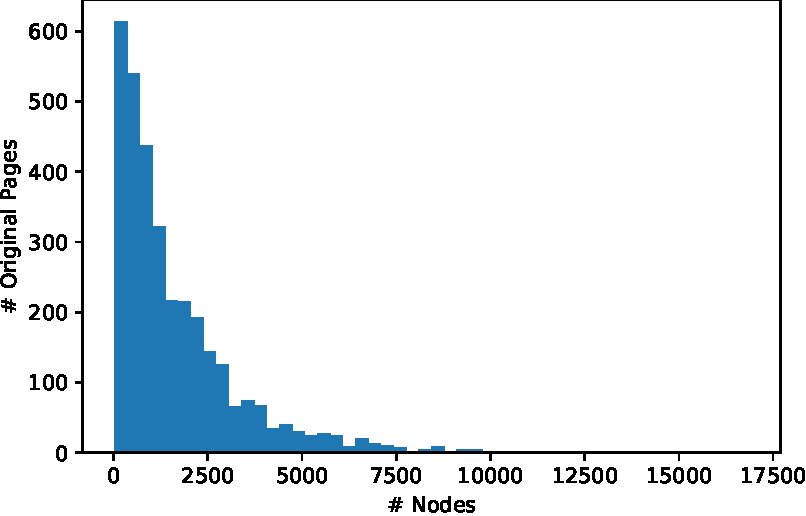
\includegraphics[width=.8\linewidth]{erratum/distribution}
  \caption{Distribution of DOM sizes (in number of nodes) in the \textsc{Mutation} dataset.}
  \label{fig:distribution}
\end{figure}

This dataset was built with an automation tool that we made available along with its source code~\ref{erratum:sec:conclusion}.
From a given list or source URLs, our tool creates a dataset of randomly mutated web pages following the above-described approach.

\subsubsection{Buidling the {\sc Wayback} dataset.}\label{waybackDataset}
This dataset encloses a list of $(D, D')$ DOM pairs where $D$ and $D'$ are two versions of the same page (\emph{e.g.}, \textit{google.com} between 01/01/2013 and 01/02/2013).
Two versions can be separated by different gaps in time.
In this section, we explain how we used the Wayback API to build this dataset.
The Wayback API can be used to explore past versions of websites.
The two endpoints we used to build the dataset can be modeled as the following functions:
\begin{align*}
versionsExplorer &::& (url, duration)  & \to & timestamp[] \\
versionResolver  &::& (url, timestamp) & \to & document
\end{align*}
The \textit{versionsExplorer} retrieves the list of available snapshots between two dates, while the \textit{versionResolver} returns the snapshot of a given \textit{url} at the requested timestamp.

Using these endpoints, for each website URL considered, we:
\begin{compactenum}
\item retrieved the timestamps of all versions between 2010 and today using the \textit{VersionExplorer},
\item generated a list of all pairs of timestamps with one of following differences in days ($\pm 10\%$): $\text{[7, 15, 30, 60, 120, 240, 360]}$,
\item picked up to $1,000$ random elements from the list of timestamps pairs,
\item resolved each selected timestamp pair using the \textit{versionResolver}.
\end{compactenum}

Similarly to the {\sc Mutation} dataset, the URLs we fed to our algorithm were taken from the Top\,1K Alexa.
Since both datasets are based on the same set of URLs (taken from Alexa), the distribution of the {\sc Wayback} dataset is very similar to the {\sc Mutation} one (cf. Figure~\ref{fig:distribution_wayback}).

\begin{figure}[h]
  \centering
  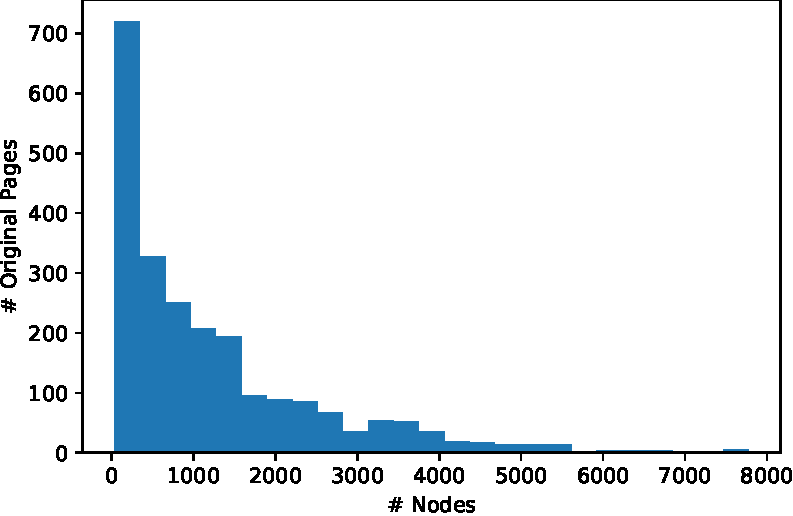
\includegraphics[width=.8\linewidth]{erratum/distribution_wayback}
  \caption{Distribution of DOM sizes (in number of nodes) in the \textsc{Wayback} dataset.}
  \label{fig:distribution_wayback}
\end{figure}

\subsubsection{Selecting the elements to repair.}
\erratum{} and WATER operate in different ways.
\erratum{} takes two trees $(D, D')$ and returns a matching between each element of the trees, thus solving any possible broken locator between $D$ and $D'$.
The algorithm extracted from WATER is a more straightforward solution to the locator repair problem as formally described (cf. Section~\ref{locator_repair_problem}): it takes a pair of DOM versions $(D,D')$ and an element $e \in D$ as input and returns an element $e' \in D'$ (or $null$ if it fails to find any candidate for the matching).

Consequently, in the case of the WATER algorithm, the following question arises: given a pair $(D, D')$ taken from the DOM version dataset, which elements of $D$ should be picked for repair? 
Ideally, we would try to locate every element of $D$ in $D'$ to obtain a comprehensive comparison with \erratum.
Unfortunately, the computation times of WATER make it impractical to locate every single element from $D$ in $D'$.
Selecting realistic targets for locators is a non-obvious task since many elements in the DOM would not be targeted in a test script (\emph{e.g.}, large container blocks, invisible elements, aesthetic elements).
Therefore, for each version pair, we randomly select up to $15$ clickable elements from $D$.
We focus on clickable elements as this is the most common use case for web UI testing (to trigger interactions), and WATER has specific heuristics to enhance its accuracy on links.
By considering clickable elements, we
\begin{inparaenum}
    \item make sure to choose realistic elements, and
    \item compare to WATER on its most typical use case.
\end{inparaenum}

Regarding the sample size, considering $15$ elements per web page leads to selecting 34,000+ elements in both datasets.
As the average number of nodes per web page in each dataset is around $1,500$, this means that there are more than 3.6M candidate locators for repair in each dataset.
Therefore, the confidence interval at 95\,\% of the measurements applied to the 34K sample of located elements is 0.5\,\%. 

\subsection{Evaluating of the Matched Elements}\label{erratum:sec:manualLabeling}
On the {\sc Mutation} dataset, the signatures attributes are preserved after mutations (but ignored when applying either locator repair solution), thus providing the ground truth matching between the DOMs of a version pair.

For the {\sc Wayback} dataset though, this information is not available.
For each version pair $(D, D')$, the evaluation of both solutions yields to a list of suggested matching $(e, e'_{ERRATUM})$ and $(e, e'_{WATER})$ where $e \in D$ and $e'_{ERRATUM}, e'_{WATER} \in D'$.
In both cases, $e'$ may be null in case no matching was found.
Given the above situation, the labeling process consists of determining whether the matching element of $e$ is $e'_{ERRATUM}$, $e'_{WATER}$, or neither.
In many cases, $e'_{ERRATUM} = e'_{WATER}$ (consensus).
We choose to focus our manual labeling effort on cases where WATER and \erratum{} disagree and assume that both solutions are right otherwise.

Thus, to label the disagreements between \erratum{} and WATER, we developed a web application (cf. Figure~\ref{fig:disagreement}) to display the identified elements on both versions of the DOM version pair and label the matching as either correct or wrong.
% A screenshot of this application is depicted in Figure~\ref{fig:disagreement}.

\begin{figure*}
  \begin{center}
  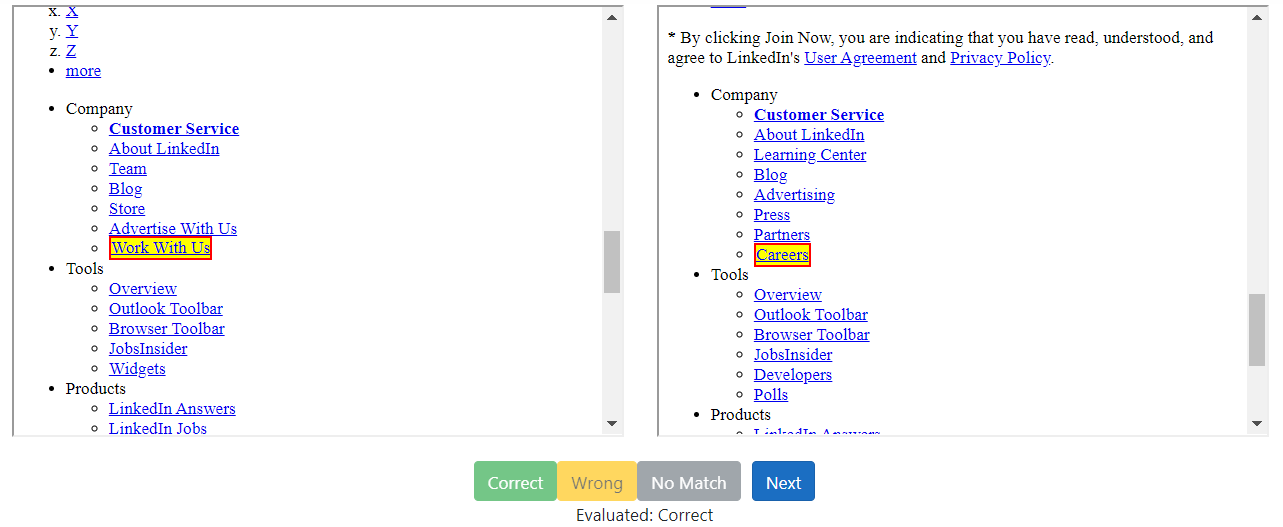
\includegraphics[width=1.1\linewidth]{erratum/disagreement}
  \caption{Labeling a given element matched by \erratum{} on two versions of the \textsf{Linkedin} homepage. The screenshot comes from the visual matching application we created to manually label disagreements between \erratum{} \& WATER.}
  \label{fig:disagreement}
  \end{center}
\end{figure*}

When we defined the similarity equivalence between two elements (cf. Definition~\ref{def:similarity}), we mentioned the potential subjective part of the measure.
To lessen this subjective part and label the proposed matchings as objectively as possible, we systematically recommended the following guidelines:
\begin{compactenum}
    \item Sometimes, matched elements are not visible (it happens when the visibility of some parts of the page is triggered dynamically).
    In this case, if elements in both versions are not visible, the locator is skipped, otherwise, the matching is considered as \textsf{mismatch};
    \item Sometimes, a link appears in different locations on the website (often sign-in links).
    Matching two such links from different locations is considered as wrong even though the two links might be assumed to have a similar semantic value.
    Therefore, we always consider the surrounding of the located element to judge whether the matching is \textsf{correct} or \textsf{mismatch}.
%     \item List of records is particularly challenging for repair solutions. For example, \textit{YouTube} displays a list of videos. These videos are not the same from one day to another. Repair solutions often tend to match such videos according to their position in the grid. While this a valuable result, we decided to label such matches as \textsf{mismatch} since the matched elements do not strictly have the same semantic value.
\end{compactenum}

% The above list is an exhaustive list of non-trivial cases encountered during manual labeling.
% The last element---list of records---highlights the limits of state-of-the-art approach for locator repair.
% In the context of web testing, the systematic labeling policy that we applied consisted in favoring semantics (\emph{e.g.}, the content of a video) over structure (its position on the grid, cf. similarity definition~\ref{def:similarity}).
% Assuming that test data (\emph{e.g.}, a list of videos) is stable over time, a semantic similarity matching should thus detect and follow the structural changes of a page over time by leveraging the semantic stability to repair the broken locator of a given element.
% This situation points towards the insufficiency of the underlying model used in existing locator related solutions and will be the object of further studies (see Section~\ref{erratum:sec:perspectives}).

% We discuss future possible solutions in Section~\ref{erratum:sec:conclusion}.

\section{Empirical Evaluation}\label{erratum:sec:evaluation}
This section evaluates locator repair solutions along with two criteria, accuracy and performance, to answer our research questions.

\subsection{Evaluation of Repair Accuracy}
In this section we answer RQ.\ref{rq:performance}: 
How does \erratum perform in solving the locator repair problem (RQ.\,\ref{locator_repair_problem}) when compared to state-of-the-art solutions?

\vspace{6pt}\noindent{\bf Repair accuracy on the \textsc{Mutation} dataset.}
Figure~\ref{fig:mutation_boxplot} summarizes the distribution of the accuracy of \erratum{} and WATER as a violin plot over the $3,291$ version pairs of our {\sc Mutation} dataset.
For each version pair $(D, D')$, the reported accuracy ratio corresponds to the ratio of the $15$ selected elements from $D$ that are accurately located in $D'$. The figure shows

\begin{figure}[]
  \centering
  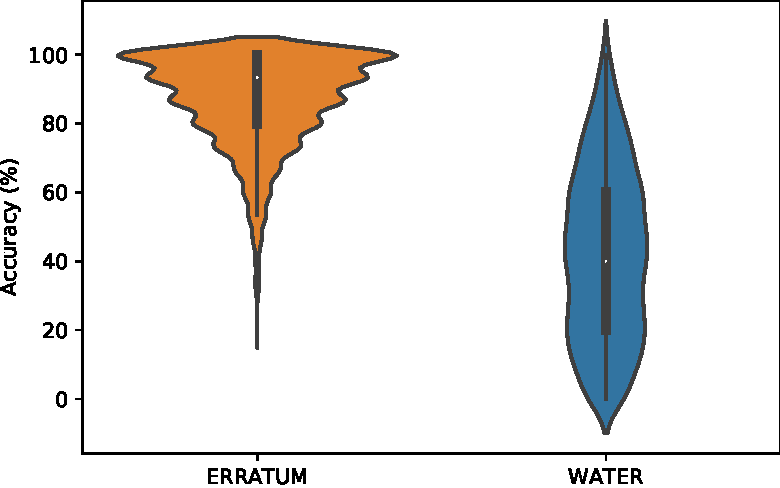
\includegraphics[width=.7\linewidth]{erratum/boxplotWaterVsSFTM}
  \caption{Accuracy distribution of \erratum{} and WATER on the \textsc{Mutation} dataset.}
  \label{fig:mutation_boxplot}
\end{figure}

% One can observe that Figure~\ref{fig:mutation_boxplot} reports on a significant difference in favor of \erratum{}. 
There are two ways a repair solution can fail to locate an element $e \in D$ in $D'$: 
\begin{inparaenum}
    \item a \textsf{mismatch}, when the original element $e \in D$ has been matched to the wrong element $e' \in D'$, or
    \item a \textsf{no-match}, when the algorithm does not manage to locate $e$ in $D'$. 
\end{inparaenum}
In case of failure, a \textsf{no-match} is always preferred to a \textsf{mismatch}, since a \textsf{no-match} alerts the developer about failure.
Thus, considering the two classes of errors on the {\sc Mutation} dataset, Table~\ref{tab:mismatch} summarizes the ratio of \textsf{no-match} and \textsf{mismatch} reported by both solutions.
In particular, the data shows a significant advantage in favor of \erratum when it comes to reducing locator mismatches, compared to WATER.

\begin{table}[H]
    \caption{Errors distribution of \erratum{} and WATER on the \textsc{Mutation} dataset.}\label{tab:mismatch}
    \centering
    \resizebox{.6\linewidth}{!}{%
        \begin{tabular}{|c|rr|rr|}
        \cline{2-5}
        \multicolumn{1}{l|}{ } & \multicolumn{2}{c|}{\bf \erratum} & \multicolumn{2}{c|}{\bf WATER} \\
        \cline{2-5}
        \hline
        \textsf{correct} & $42,876$ & $(87.0\%)$ & $20,740$ & $(42.1\%)$ \\
        \textsf{mismatch} & $4,420$ &  $(9.0\%)$ & {\color{red}$26,820$} & {\color{red}$(54.4\%)$} \\
        \textsf{no-match} & {\color{editorGreen}$2,009$} & {\color{editorGreen}$(4.0\%)$} & $1,745$ & $(3.5\%)$ \\
        \hline 
        \hline
        \bf Total: & $49,305$ & $(100\%)$ & $49,305$ & $(100\%)$ \\
        \hline 
        \end{tabular}%
    }
\end{table}

To further understand which factors influence the accuracy of \erratum and WATER (RQ.\ref{rq:influenceFactors}), we studied the evolution of accuracy according to three factors:
\begin{inparaenum}
    \item the type of mutations applied,
    \item the size of the DOM (number of nodes) of the original page $D$, and
    \item the mutation ratio applied to the original page $D$ to obtain the mutant $D'$.
\end{inparaenum}

First, to assess the impact of the mutation type on the accuracy of \erratum and WATER, we used a constrained version of the \textsc{Mutation} dataset with only one mutation operation applied for each mutant. 	
In the original \textsc{Mutation} dataset, a mutant $D'$ of a page $D$ is obtained by picking a random number $l$ of random nodes $n_1, n_2...n_l \in D$ and applying a random mutation type (cf. Table~\ref{table:mutations_used}) to each node.
In the constrained version, we use the same original pages $D$, but select a single random mutation operation per mutant $D'$.
We then apply the mutation operation to $l$ randomly selected nodes: $n_1, n_2...n_l$. 
For each original page $D$, the result is a list of mutants such that each mutant $D'$ was obtained using only one mutation operation on a random amount of random nodes.
Figure~\ref{fig:mutationTypeAnalysis} depicts the sensitivity of both locator repair solutions on this alternative dataset.
The vertical lines on top of each bar represent the confidence interval.
The figure highlights that \erratum is almost exclusively sensitive to structural mutations.
In particular, the average accuracy of \erratum is not sensitive to content mutations on the page, which is expected since the algorithm ignores the content of the nodes by default.
The very low sensitivity of \erratum to attributes related mutations is more surprising as attributes account for a major part of the similarity metric of the algorithm.
For this reason, we believe that the mutation of attributes might have more impact when combined with structural mutations, which does not happen in the constrained \textsc{Mutation} dataset.
% While results obtained on this constrained dataset give 

\begin{figure}[]
  \centering
  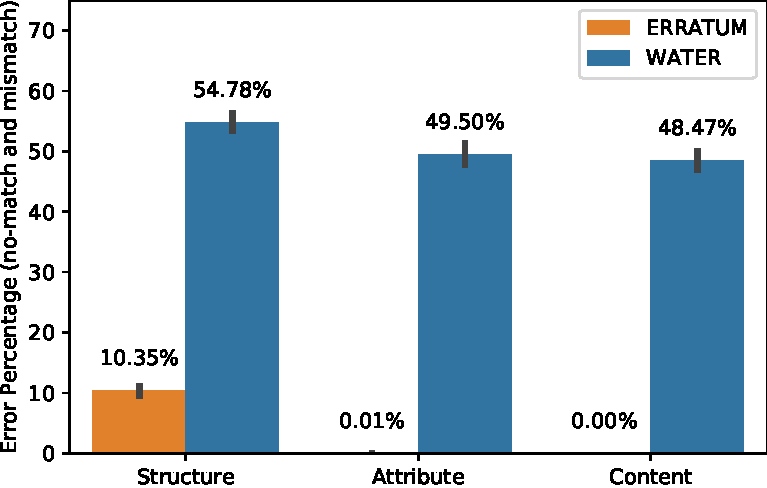
\includegraphics[width=.8\linewidth]{erratum/mutationTypeAnalysis}
  \caption{Error percentage according to the mutation type.}
  \label{fig:mutationTypeAnalysis}
\end{figure}

Then, regarding the impact of the size of the DOM, our analysis concludes that
WATER loses accuracy when the number of nodes increases (cf.
Figure~\ref{fig:nbNodesAccuracy}), while \erratum{} exhibits a more stable
performance. The Spearman correlation coefficient between the error ratio of
WATER and the size of the DOM is $\rho = 0.41$ compared to $0.28$ for \erratum{}.
Interestingly, while \erratum{} correlates rather strongly ($\rho = 0.46$) with the
percentage of mutation between the two DOM versions, WATER shows almost no
correlation with the same variable ($\rho = 0.12$). It means WATER is surprisingly
not impacted by the amount mutations between the versions. The dependency to the
mutation ratio of \erratum{} is easily explainable: for each match, \erratum{}
indirectly relies on structural and textual similarities in the whole DOM which
means mutations anywhere in the DOM could theoretically impact the scores on
which \erratum{} relies to compute a matching. Conversely, WATER approach is
fundamentally more local to the element to match. We believe these are key
insights in understanding the limitation of WATER when compared to \erratum{}.
For each element $e \in D$ to locate, WATER searches through all same-tag elements
in $D'$ (the \textit{candidates}) and picks the closest one to $D$, with respect
to WATER's chosen similarity metric. We believe that the sensitivity of WATER to
the number of nodes comes from the fact that the number of \textit{candidate}
matchings for a given element $e$ tends to grow with the size of the DOM, which
increases the complexity of the ordering-by-similarity task. Conversely,
additional nodes provide more "anchor" points to \erratum, partially
compensating the increase in possible combinations.

\begin{figure}[]
  \centering
  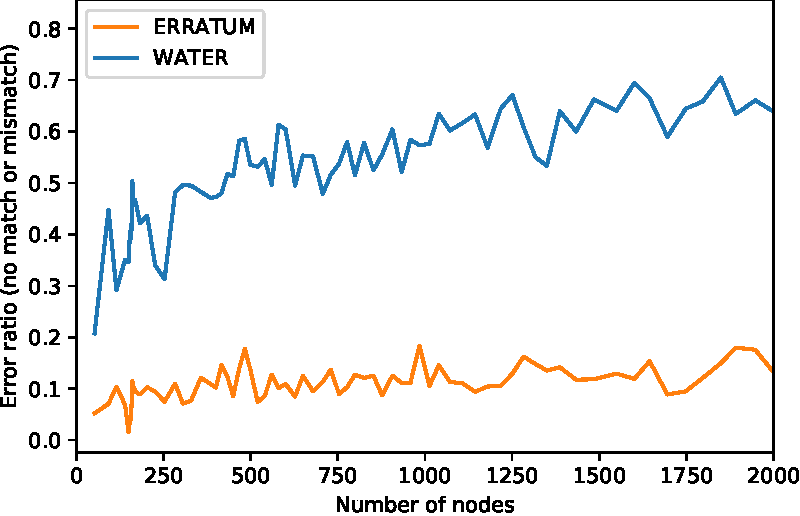
\includegraphics[width=.8\linewidth]{erratum/mutation-numberNodes-mistake}
  \caption{Errors rate evolution according to DOM size.}
  \label{fig:nbNodesAccuracy}
\end{figure}

Finally, regarding the impact of the mutation ratio ($\frac{\#mutations}{\#nodes}$), Figure~\ref{fig:erroRatioMutation} reports on how \erratum and WATER's errors evolve when increasing the number of mutations ($\#mutation$) on the original page $D$.
The figure contains more information than most common box plots, in particular: the stars indicate the average ratio, the horizontal orange lines, the medians whose values also appear above the boxes.
As expected, both solutions lose accuracy when the mutation ratio increases, but one can still observe that \erratum demonstrates a significant advantage over WATER, no matter the mutation ratio, and exhibiting only 20\% of errors on average (against 67\% for WATER) when the ratio of mutation exceeds 20\% of the nodes.

\begin{figure*}[]
  \centering
  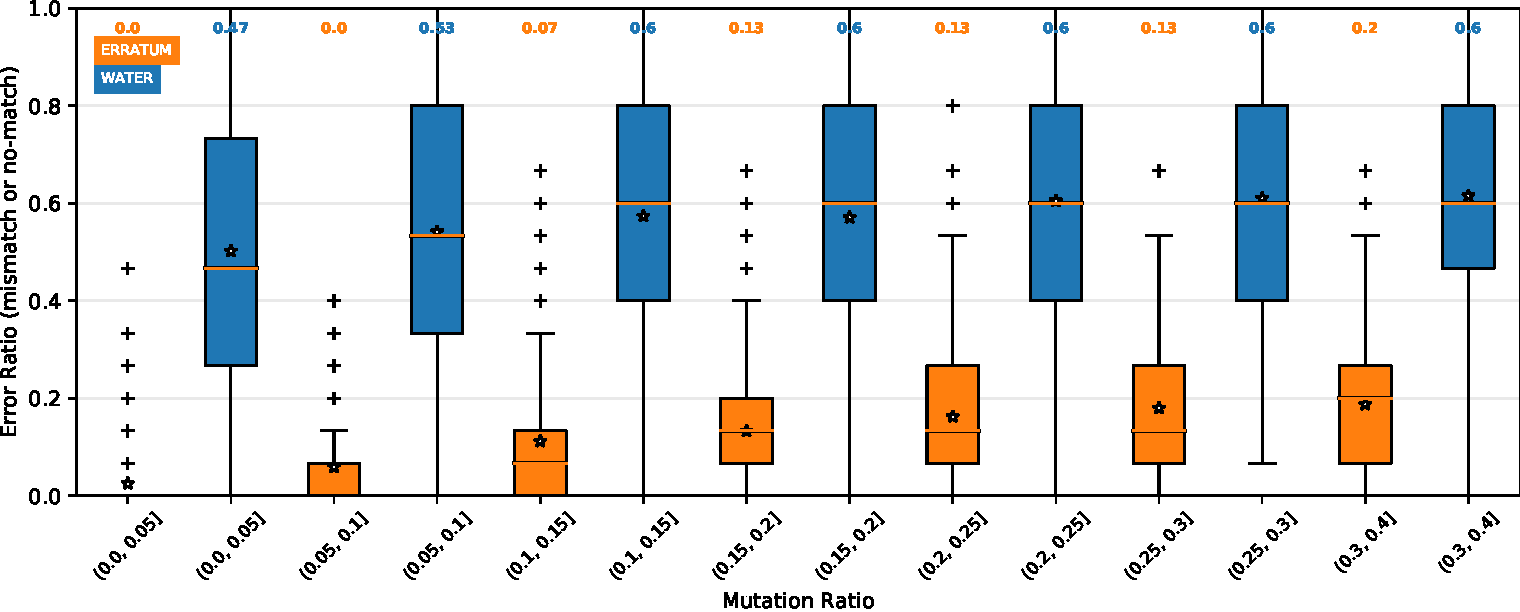
\includegraphics[width=1\linewidth]{erratum/errorPerMutationRatio}
  \caption{Errors rate evolution according to the mutation ratio.}
  \label{fig:erroRatioMutation}
\end{figure*}


\vspace{6pt}\noindent{\bf Repair accuracy on the \textsc{Wayback} dataset.}
Since the {\sc Wayback} dataset does not provide any ground truth matching, we had to manually label the results of the evaluation.
We ran both algorithms on the same 34,421 elements.
For each element $e \in D$, \erratum and WATER returned $e'_{S}$ and $e'_{W} \in D' \cup \emptyset$, respectively.
In 49.0\% of cases, \erratum and WATER agreed on a matching element ($e'_{S} = e'_{W} \ne \emptyset$).
In 13.6\% of cases, no solution found a matching element ($e'_{S} = e'_{W}= \emptyset$).
In 37.4\% of cases, \erratum and WATER disagreed on the matching element ($e'_{S} \ne e'_{W} \text{ and } (e'_{S}, e'_{W}) \ne (\emptyset, \emptyset)$).

A sample of $366$ matchings out of the $14,784$ disagreements where labelled by web testing experts, which corresponds to a 5\% confidence interval at 95\%.
Table~\ref{tab:labels} reports on the results of the manual labeling (for disagreements), thus assuming that both WATER and \erratum are correct whenever they agree.

\begin{table}[h]
    \caption{Confusion matrix on the \textsc{Wayback} dataset.}\label{tab:labels}
    \centering
    \resizebox{.65\linewidth}{!} & \multicolumn{1}{r|}{1.5\%} & \multicolumn{1}{r|}{1.4\%} & \color{red}{51.9\%} \\
        \cline{2-5}
        \multicolumn{1}{|l|}{} & \multicolumn{1}{c|}{\sf mismatch} & \multicolumn{1}{r|}{26.5\%} & \multicolumn{1}{r|}{5.5\%} & \multicolumn{1}{r|}{3.3\%} & 35.3\% \\
        \cline{2-5}
        \multicolumn{1}{|l|}{\multirow{-3}{*}{\rotatebox[origin=c]{90}{\scriptsize \textbf{WATER}}}} & \multicolumn{1}{c|}{\sf no-match} & \multicolumn{1}{r|}{2.8\%} & \multicolumn{1}{r|}{1.9\%} & \multicolumn{1}{r|}{8.1\%} & 12.8\% \\
        \cline{1-5}
        \cline{1-5}
         & & \color{editorGreen}{78.3\%} & 8.9\% & 12.8\% & 
        \end{tabular}%
    }
\end{table}

We further investigated the causes of \textsf{no-match} cases reported by \erratum{} to assess if these specific cases could be matched by experts.
% Additionally, we wondered what part of the elements labeled as no-match by SFTM would actually be considered as no-match for humans. 
As part of the \textsc{Wayback} experiment, we thus included \erratum's \textsf{no-match} cases in our labelling application (cf. Figure~\ref{fig:disagreement}) and requested the participants to eventually propose a matching element if a \textsf{no-match} was reported by \erratum{}.
The result of this evaluation, summarized in Figure~\ref{fig:nomatch-analysis}, highlights that a majority of \textsf{no-match} are accurately labeled as such by \erratum{}, since the participants could not propose a matching element in the target web page. 
For the few cases where the participants proposed a matching element, we observed that the structure of the DOM tree where subject to many mutations, thus misleading \erratum{} as already observed in Figure~\ref{fig:mutationTypeAnalysis}.
% When SFTM mistakenly labeled an element as a no-match we tried to understand what led SFTM to fail.
% While it is sometimes hard to understand due to the size of the DOMs considered, in most situation, it seemed SFTM had trouble when both the structure and the labels in the tree have significantly changed.

\begin{figure}[]
  \centering
  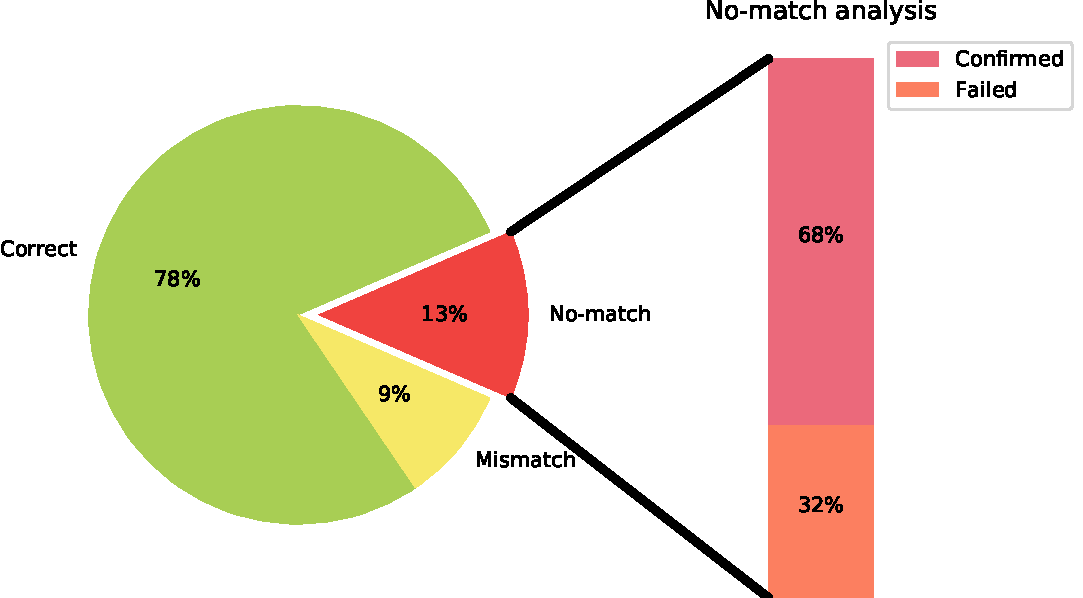
\includegraphics[width=.75\linewidth]{erratum/nomatch-analysis}
  \caption{Analysis of matches labeled as \textsf{no-match} by \erratum{}.}
  \label{fig:nomatch-analysis}
\end{figure}


\vspace{6pt}\noindent{\bf Comparison of repair accuracy.}
Interestingly, as shown in Table~\ref{table:datasets_comparison}, the accuracy of \erratum on the {\sc Wayback} dataset ($78.3\,\% \pm 5\,\%$) is $8.7\%$ inferior to the accuracy obtained on the {\sc Mutation} dataset ($87.0\%$), while the accuracy of the WATER algorithm is better on the {\sc Wayback} dataset ($51.9\,\% \pm 5\,\%$) than on the {\sc Mutation} dataset ($42.1\,\%$) by $9.8\,\%$.
We believe the difference observed between the two datasets is because real-life mutations might not be uniformly distributed.
In particular, regarding our sensitivity analysis with regards to types of tree mutations (cf. Figure~\ref{fig:mutationTypeAnalysis}), one can guess that real-life websites are more subject to \emph{content} and \emph{attribute}-related mutations than \emph{structure}-based mutations (cf. Table~\ref{table:mutations_used}), as the former do not affect the accuracy of \erratum{}.
However, since we miss the ground truth for the {\sc Wayback} dataset, we cannot assess this hypothesis and the distribution of real-life mutations.

\begin{table}[h]
    \caption{Accuracy summary across datasets.}
    \label{table:datasets_comparison}
    \centering
    \resizebox{.5\linewidth}{!}{%
        \begin{tabular}{|l|c|c|}
        \cline{2-3}
        \multicolumn{1}{l|}{ } & {\sc Mutation} & {\sc Wayback} \\
        \cline{2-3}
        \hline
        \bf \erratum & 87.0\% & {78.3 $\pm$ 5\%} \\
        \hline
        \bf WATER    & 42.1\% & {51.9 $\pm$ 5\%} \\
        \hline
        \end{tabular}
    }
\end{table}

\subsection{Mutations in the {\sc Wayback} Dataset}
To assess the accuracy of \erratum on both datasets, we study the nature of the changes occurring between two versions of a given page in the \textsc{Wayback} dataset.
The changes applied along versions of pages available in the \textsc{Wayback} dataset are not labeled, thus lacking a ground truth.
% 
The robust locator benchmark (cf. Section~\ref{erratum:sec:benchmark}) assumes the input datasets as the ground truth to evaluate \erratum on the locator repair problem.
Conversely, this section assumes the matching algorithm exploited by \erratum---\emph{i.e.}, SFTM---to be correct and uses it to label the mutations observed in the \textsc{Wayback} dataset.
% 
To do so, we estimate the number and types of mutations between each pair of web pages $(D, D')$ by leveraging the resulting matching $M = sftm(D,D')$.
The following table lists the considered mutation types, considering $\forall e \in D$ and $\forall e' \in D'$, where $p(e)$ is the parent of $e$ and $\lambda(e)$ is the label of $e$:
\begin{table}[h]
\centering
\begin{tabular}{|l|l|l|}
% \cline{2-3}
\hline
Label        & Mutation                                          & Category \\ \hline
\hline
\sf addition & $\nexists e | (e, e') \in M$                      & Structural \\ \hline
\sf removal  & $\nexists e' | (e, e') \in M$                     & Structural \\ \hline
\sf move     & $(e, e') \in M$ and $(p(e), p(e')) \notin M$      & Structural \\ \hline
\sf relabel  & $(e, e') \in M$ and $\lambda(e) \neq \lambda(e')$ & Relabel \\ \hline
\end{tabular}
\end{table}


\vspace{6pt}\noindent{\bf Dataset Consolidation.}
The robust locator benchmark considers a subset of the \textsc{Wayback} dataset, manually labeled by experts.
However, during this process, potential inconsistencies observed in rendered web pages were ignored by experts.
% 
Therefore, before analyzing the full \textsc{Wayback} dataset, one should discard such inconsistencies between unrelated web pages, including cases where:
\begin{inparaenum}[\em (a)]
\item one of the versions can be an error page or a redirection page,
\item the website may shown "in construction" or may have closed between the two snapshots.
\end{inparaenum}  
% 
For this reason, we apply two heuristics to prepare the dataset by removing all the pairs where:
\begin{compactenum}
  \item one the two versions has less than 30 nodes, reflecting one of the above inconsistencies.
  For example, even a minimalist web page, like Google, contains more than 250 nodes;
  \item the absolute ratio of sizes between the two versions exceeds 40\% which
  selects approximately 90\% of the dataset (see
  Figure~\ref{fig:sizeDiffRatioDistribution}). When this ratio is large,
  comparing the two pages is likely to be conceptually irrelevant.
\end{compactenum}

While the initial \textsc{Wayback} dataset contains $19,161$ pairs of web pages, the application of the above rules leads to a consolidated dataset of $8,641$ pairs. % After the first filter it is 9,580 and after the second
Figure~\ref{fig:sizeDiffRatioDistribution} reports on the distribution of ratios of web page versions in the consolidated \textsc{Wayback} dataset.

\begin{figure}
  \centering
  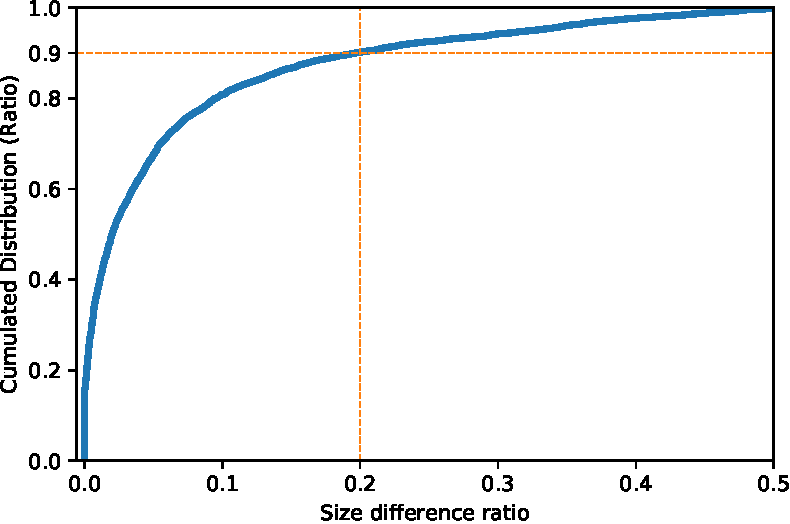
\includegraphics[width=.8\linewidth]{erratum/sizeDiffRatioDistribution}
  \caption{Cumulative Distribution of ratios between two versions of web pages.
    The orange dotted lines show the threshold used in this experiment}
  \label{fig:sizeDiffRatioDistribution}
\end{figure}


\vspace{6pt}\noindent{\bf Mutation Frequency.}
Figure~\ref{fig:mutationAmountAnalysis} further analyzes the above dataset by reporting on the ratio of mutations by category occurring between two versions of a web page.

\begin{figure}[]
  \centering
  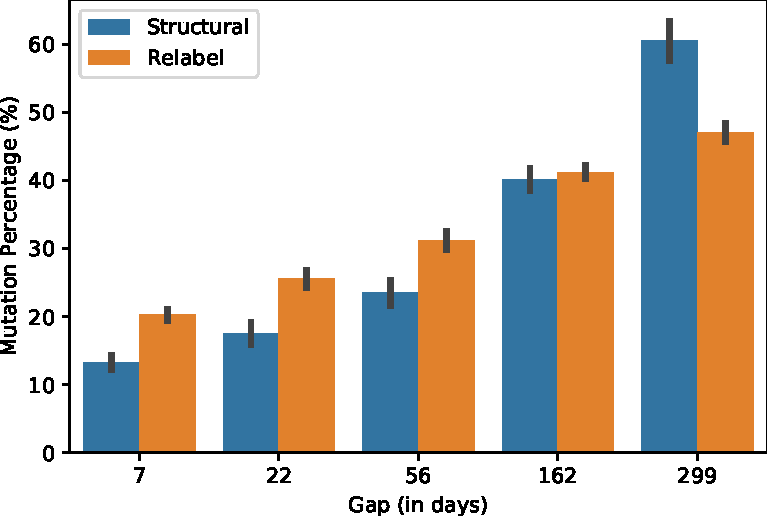
\includegraphics[width=.8\linewidth]{erratum/mutationAmountAnalysis}
  \caption{Mutation ratio between two \textsc{Wayback} snapshots depending on gap duration.}
  \label{fig:mutationAmountAnalysis}
\end{figure}

As expected, the mutation ratio increases with the gap between the versions.
Most importantly, the average mutation ratio in the \textsc{Wayback} dataset is
60\%, i.e. in average, 60\% of the nodes have mutated between two versions $D$
and $D'$ from the Wayback dataset. This mutation ratio is significantly higher
than the average amount of mutations in the \textsc{Mutation} dataset: 20\%.
This difference is probably an important factor justifying the differences of
accuracy measured on both datasets.
% 
Comparing versions with large gaps is practical because it ensures there will be
differences between the versions.
In addition, it provides interesting insights about the frequency of changes on popular web pages.
However, in the context of web testing, the mutation ratio between two consecutive versions is unlikely to reach 60\%, in particular when adopting test-driven developments.

\vspace{6pt}\noindent{\bf Mutation Labels.}
% Using the table described above, we study the mutation labels occurring between web page versions.
Figure~\ref{fig:mutationTypeRatios} further describes the distribution of mutation labels in the \textsc{Wayback} dataset.
The figure highlights that \textsf{relabel} is the most common mutation, while \textsf{move} is quite rare.
This result can be explained by the following observations:
\begin{inparaenum}
  \item when a subtree is moved, only one move is accounted even if the visual change may appear as important, and
  \item the SFTM algorithm is particularly robust to relabels, which could also be a factor explaining the observed ratio.
\end{inparaenum}

\begin{figure}[]
  \centering
  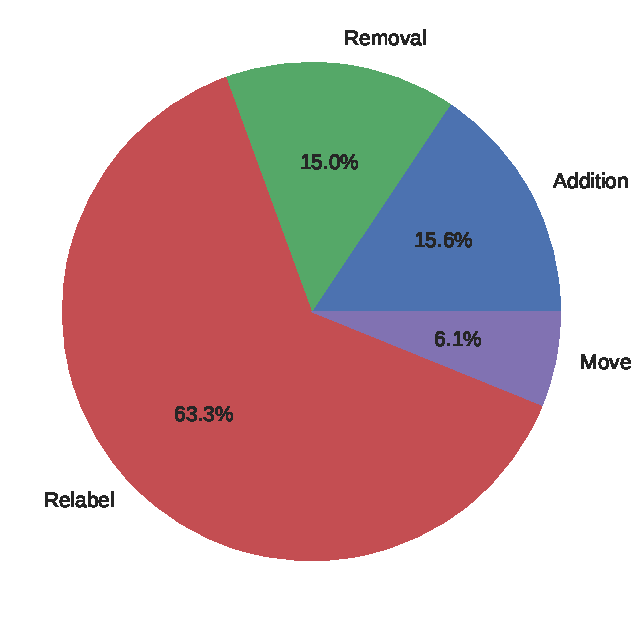
\includegraphics[width=.65\linewidth]{erratum/mutationTypeRatios}
  \caption{Distribution of mutation labels in the \textsc{Wayback} dataset.}
  \label{fig:mutationTypeRatios}
\end{figure}



\subsection{Repair Time Evaluation}\label{erratum:sec:computation_time}
In Figure~\ref{fig:computation}, we compare the computation times of \erratum{} and WATER.
The results have been obtained by running both algorithms on the same server containing 252\,GB of RAM and an Intel(R)~Xeon(R)~CPU E5-2660\,v3 @ 2.60\,GHz.
% It is interesting to note that, even though the theoretical worst-case complexity of SFTM is $O(N\sqrt N)$ (where $N$, is the number of nodes), the observed computation times of \erratum rather seem to be linear with the number of nodes.

\erratum works differently than WATER: while WATER matches one single element at a time, \erratum matches all elements at once.
One can observe that WATER is thus faster at locating a single element than \erratum is at locating all elements.
However, when the number of locators to repair grows, the computation time of WATER evolves proportionally, while the computation time of \erratum remains the same.

\begin{figure}[]
  \centering
  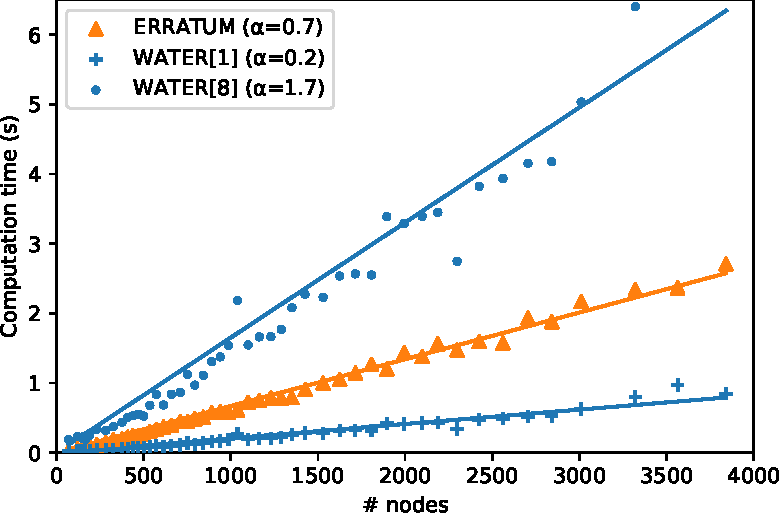
\includegraphics[width=.8\linewidth]{erratum/computationTime}
  \caption{Repair time evolution according to DOM size.}
  \label{fig:computation}
\end{figure}

More specifically, we compare the evolution of the performance coefficient ($\alpha$) when increasing the number of locators to repair in a web page.
Figure~\ref{fig:comparisonLinearCoefficients} plots these coefficients for \erratum and WATER, so that we can establish that \erratum{} becomes more efficient than WATER as soon as there are more than 3 locators to repair in a web page.

\begin{figure}[]
  \centering
  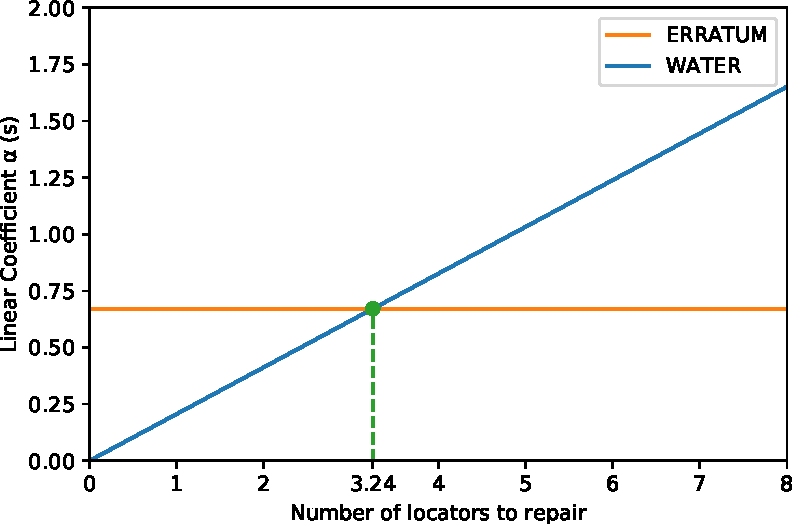
\includegraphics[width=.75\linewidth]{erratum/linearRegression}
  \caption{Performances of \erratum and WATER.}
  \label{fig:comparisonLinearCoefficients}
\end{figure}



% \section{Discussion}
% While we focus on finding a solution to the locator repair problem, such a solution will not allow repairing a broken test by itself
% As illustrated in Figure~\ref{fig:locator_repair}, fixing a test involves several steps and repairing the locator is only one of them.
% However, in previous studies, it has been shown that the locator repair problem is the most challenging part of the repairing process and WATER~\cite{choudhary2011water} describes algorithms for all the other parts of the process.


\subsection{Threats to Validity}\label{erratum:sec:threats}
% Our dataset contains the homepages taken from  the Top\,1k Alexa websites.
% The fact that our qualitative evaluation has only been conducted on \textit{homepages} might have biased the results since some page types (like product list or research results) are likely less present in this class of web pages.
As described in Section~\ref{erratum:sec:manualLabeling}, the \textsc{Wayback} dataset does not include a ground truth (perfect matching).
This is why we had to manually label a representative sample of the matchings obtained on this dataset, which might have introduced some bias.
To mitigate this bias, we recommended systematic and consistent decisions to label the data (cf. Section~\ref{erratum:sec:manualLabeling}). 

All our experiments with \erratum adopt the default FTM parameters, as recommended by~\cite{Kumar2011_FTM}.
Nonetheless, a thorough parameter sensitivity study would probably result in further improving the accuracy of \erratum.
Given the results we obtain on a wide diversity of web pages evolutions, we believe that this parameter tuning would only positively and marginally impact the accuracy of \erratum.
% \erratum uses SFTM's default parameters.
% \cite{Kumar2011_FTM} and \ref{chap:sftm} already discuss the tuning of the different parameters used in FTM and SFTM, respectively.
% In our evaluation, we found that these parameters allowed for an already significant improvement over the state of art over a very large array of web pages: 
% \begin{inparaenum}
% \item threshold function $f(N) = \sqrt{N}$, 
% \item no-match cost $w_{nomatch} = 5$, 
% \item $\gamma = 0.75$,
% \item $\beta = 0.75$,
% \item number of metropolis iterations: $N_{metropolis} = 100$, and
% \item propagation weights: $w_p = [0.6, 0.3, 0.1]$
% \end{inparaenum}
% As stated by \ref{chap:sftm}, $f$ and $N_{metropolis}$ allow to balance accuracy and computation times, $w_{nomatch}$ the no-match and mismatch rates and $\gamma$ the tendency to rather explore or exploit in the metropolis algorithm.
% From all the steps involved, this article focuses on the particularly challenging \emph{locator repair} problem---\emph{i.e.}, relocating an element taken from the original page in its new version.
% However, since our experiments were led on a very large variety of websites, our results showing a significant increase in accuracy should be applicable to an equally wide array of use case with the parameters we provided.

In terms of repair time, we discussed the absolute value of repair time for both solutions.
However, these values highly depend on the way each tool was implemented and the machines on which the simulations were run.
To limit this bias, both solutions were executed on the same Node.js runtime version deployed in the same environment to ensure a proper comparison.

\section{Applying \erratum}\label{erratum:sec:perspectives}
We have studied how \erratum{} can help in solving the existing locator repair problem, which is a common problem in web automation scripts.
In this section, we envision a more interactive development process made possible by \erratum{}.

When developing a web automation script, a developer typically opens the page under test in the browser, visually locates the element to interact with and then encodes (or generates) a locator for this element.
The locator is then used in the web automation script to select the target element and interact with it.
% 
Based on the results achieved by \erratum{}, the perspectives for this work include a new layer of abstraction to the target selection.
In this new layer, web automation scripts no longer need to explicitly locate elements on the page directly, but only locate elements using a back-end service $H$:
\begin{compactenum}
    \item each web page $D$ under automation is registered in $H$,
    \item for each registered web page $D$, $H$ exposes a visual interface
    allowing the developer to visually select an element $e$ and generate a
    unique identifier $e_{id}$ (e.g UUID),
    \item in the web automation script, instead of using a manually encoded (or generated) XPath or CSS locator to select the target element $e$, the developer sends $(D, e_{id})$ to $H$'s API, which returns an absolute XPath selecting the target element $e$,
    \item when a web page $D$ registered in $H$ evolves into a new version $D'$, \erratum{} is automatically used to relocate all registered elements $e_{id}$ in $D$ with their matching elements in $D'$,
    \item whenever \erratum{} fails (or lacks confidence) to relocate an element, the developer is notified and invited to visually relocate the broken locator.
\end{compactenum}

This approach differs from the test repair approach described in the original WATER article. 
In the test repair approach, the locator repair is triggered by the failure of one of the test scripts.
Once such a test script fails, the test repair solution attempts to determine the cause of the breakage and if it is a locator, repair the locator.
The approach we suggest in this section does not include the analysis of any automation script, as locators are updated whenever the page changes.

% Ensuring that web test scripts do not contain any hardcoded locators means that, whenever a web test script breaks because of a locator breakage (which accounts for $74\%$ of test breakage), the web test script will not have to be modified, which could constitute a considerable gain of time for developers.

In many cases, the locator breakage occurs silently (the locator is mismatched
and the consequences happen only later in the test
script)~\cite{stocco2018visual}. In these situations, it is harder to locate the
origin of the breakage from the test script. The silent breakage problem happens
because when using xPath locators to relocate $e$ in $D'$, the xPath query
either succeed or fail. There is no indication on the confidence of the
relocation that would help to detect a mismatch. On the opposite, Using
\erratum{}, every individual match between two elements $e$ and $e'$ has an
associated cost $s(e, e')$ that can be used as a confidence level to avoid
mismatch.

In addition to the obvious gain in time that having a visual-based breakage and
repair solution provides, the \erratum-based notification process described
above would thus help to detect possible breakage before the scripts are even
run, thus diminishing the chances for a "silent breakage" to occur.

% For all state-of-the-art solutions, locating elements on pages containing list of records is really challenging (\emph{e.g.}, YouTube, Amazon). 
% This limitation shows that a binary DOM matching---\emph{i.e.}, two elements either match or not---is insufficient to model the semantics of a web page.
% In future work, we intend to leverage record detection algorithms to build an abstraction of the DOM and run our tree matching solution on the abstract DOM to improve our overall ability to intelligently identify and keep track of elements on a web page. 

\section{Conclusion}\label{erratum:sec:conclusion}
In this chapter, we considered the situation in which the evolution of a web page causes one of its associated automation scripts to break.
In the domain of automated web testing, this situation accounts for 74\% of test breakages, according to past studies~\cite{hammoudi2016record}.
% 
Our analysis of the state-of-the-art approaches on this topic contributed to formalize the key steps involved in preventing or fixing such a kind of test breakage.

While existing solutions to the locator repair problem treats broken locators individually, we rather propose to apply a holistic approach to the problem, by leveraging an efficient tree matching algorithm.
This tree matching approach thus allows \erratum{}, our solution to repair all broken locators by mapping all the elements contained in an original page, to accurately relocate each of them in its new version at once.
% 
To assess \erratum{}, we created and shared the first reproducible, large-scale datasets of web page locators, combining synthetic and real instances,\footnote{Dataset available from \url{https://zenodo.org/record/3800130\#.XrQb02gzY20}} which has been incorporated in a comprehensive benchmark of \erratum{} and WATER, a state-of-the-art competitor.\footnote{Benchmark available from \url{https://zenodo.org/record/3817617\#.XrWdqGgzaoQ}}
%
Our in-depth evaluation highlights that \erratum{} outperforms WATER, both in accuracy---by fixing twice more broken than WATER---and performances---by providing faster computation time than WATER when repairing more than 3 locators in a web test script.

Finally, we worked with the development team of a widely used open source test framework called Cerberus~\footnote{https://cerberus-testing.com/} to integrate~\footnote{https://github.com/cerberustesting/cerberus-source/commit/0a70d4cc0d70a797901652fd2b97d501bb7fa511} the Erratum approach into the test creation part of the software.
The next section describes the integration of Erratum to Cerberus and its impact on some of its users.
% Finally, we demonstrate that \erratum{} is weakly impacted by the mutation rate and DOM size of web pages, which makes it a serious candidate for being deployed in web developments.


\chapter{Integrating Erratum to Cerberus}

\section{Abstract}
Web applications are constantly evolving to integrate new features and fix reported bugs.
However, even an imperceptible change can sometimes entail significant modifications of the \emph{Document Object Model} (DOM), which is the underlying model used by browsers to render elements of a web application.
In this context, the continuous evolution of web applications makes it extremely challenging to automate test scenarios of a web application in a robust way.
More precisely, the major cause of breakages observed in integration tests are \emph{element locators}, which are identifiers used by automated tests to navigate across a DOM.
When this DOM evolves, these locators tend to break, thus causing the related tests to no longer locate the intended target elements.

So far, established test automation frameworks adopted by the industry, like \cerberus{}, only support CSS or XPath selectors to query web page elements.
Such web locators require to be manually crafted and are often fragile with regards to DOM changes, hence often requiring testers to fix the broken test scenarios in priority. 
While several solutions to this problem have been proposed in the scientific literature, to our knowledge, no locator repair or locator generator has been integrated in open-source test-automation software before.
This paper thus reports on the seamless integration of a more robust web locator in \cerberus{} by leveraging a new locator repair solution, named \erratum{}. While \erratum was originally designed to repair broken locators, this paper demonstrates how it can be extended to deliver an elegant robust locator solution that succeeds to reduce the maintenance cost of automated tests.

\section{Introduction}
The implementation of automated tests on web applications (apps) requires software engineers to locate specific elements in the DOM (\emph{Document Object Model}) of a web page.
To do so, software testers or automation/testing tools often rely on CSS (\emph{Cascading Style Sheets}) or XPath selectors to query the target elements they need to interact with.
Unfortunately, such statically-defined locators tend to break along time and deployments of new versions of a web application.
This often results in the failure of all the associated test scenarios that apply to the modified web pages.

Several existing works focus on repairing tests on GUI applications, but there are surprisingly very few test repair solutions targeting web interfaces~\cite{imtiaz2019systematic}.
These solutions either propose to \emph{i)} generate locators that are robust to changes (so-called \emph{robust locator problem}), or \emph{ii)} repair locators that are broken by the changes applied to the web pages (so-called \emph{locator repair problem}).
Unfortunately, most of the existing solutions in the literature fail to accurately fix a broken locator, thus leaving all the related automation tests as broken~\cite{hammoudi2016record}.

While we already introduced \erratum{},\footnote{\erratum{} stands for "\erratumlong{}"} as an holistic approach to the locator repair problem~\cite{brisset2021erratum}, this paper explores its extension to address the robust locator problem.
More specifically, we report on the integration of \erratum{} in an open-source test automation solution called \cerberus{}~\cite{cerberus-icst20}.\footnote{\url{https://cerberus-testing.com/}}
\cerberus{} is commonly adopted by several companies to write, organize, and run their test campaigns.
In particular, we worked in close collaboration with the web testing team of \laredoute{},\footnote{\url{https://www.laredoute.com/}} a large (846M turnover, $1,700$ employees) french online fashion retailer.

The teams we worked with acknowledged that locator breakage is a painful issue for them that even caused a whole test campaign to be cancelled.
Yet, to the best of our knowledge, none of the locator generator or locator repair solutions existing in the literature have ever been integrated in an open-source testing software.
As a matter of assessment, we observed that the concept of locator repair was unknown to all professional testers we interviewed.


The remainder of this paper is organized as follows.
Section~\ref{sec:related-work} introduces the necessary background on web locators.
% 
Then, Sections~\ref{sec:erratum} and~\ref{sec:cerberus} overview \erratum and \cerberus, respectively, while Section~\ref{sec:integration} reports on the integration of a robust locator solution in \cerberus based on \erratum.
Section~\ref{sec:impact} discusses the preliminary impact of this integration on the software development projects managed by \laredoute.
% 
% Section~\ref{sec:locator} formalizes the locator problem we address in this paper.
% Section~\ref{sec:implementation} introduces our approach, \erratum, which leverages an efficient flexible tree matching solution that we identified.
% Section~\ref{sec:benchmark} describes the locator benchmark we designed and implemented.
% Section~\ref{sec:evaluation} reports on the performance of our approach compared to the state-of-the-art algorithms.
% Section~\ref{sec:threats} discusses the threats to validity of our contribution.
Finally, Section~\ref{sec:perspectives} presents some perspectives for this work, while Section~\ref{sec:conclusion} concludes.

\section{Background}\label{sec:related-work}
\subsection{Web Element Locators}
To detect regressions in web applications, software engineers often rely on automated web-testing solutions to make sure that end-to-end user scenarios keep exhibiting the same behavior along changes applied to the system under test.
Such automated tests usually trigger interactions as sequences of actions applied on selected elements and followed by assertions on the updated state of the web page.
For example, \emph{"click on button $e_1$, and assert that the text block $e_2$ contains the text '{\tt Form sent}'"}.
To build such test scenarios, a software engineer can
\begin{inparaenum}
    \item manually write web test scripts to interact with the application,
    \item use record/replay tools~\cite{burg2013interactive,sen2013jalangi,mickens2010mugshot} to visually record their scenarios, or
    \item adopt low-code test libraries to leverage the description of actions for domain experts.
\end{inparaenum}
In all these cases, the scenario requires to identify the target elements on the page [$e_1$, $e_2$] in a deterministic way, which is usually achieved using XPath, a query language for selecting elements from an XML document.
% 
For example, let us consider the following HTML snippet describing a web form:
\begin{lstlisting}
<form method="post" action="index.php"> 
    <input type="text"   name="username"/> 
    <input type="submit" value="send"/>
</form> 
\end{lstlisting}

The following XPath snippets describe 3 different queries, which all result in selecting the submit button: \lstinline!/form/input[2]!, \lstinline!/form/input[@value="Send"]!, \lstinline!input[@type="submit"]!.
In the literature, such element queries or identifiers are named \emph{locators}~\cite{leotta2014reducing}.

In practice, automated tests are often subject to breakages~\cite{hammoudi2016record}.
While there can be many causes to test breakage, Hammoudi~\emph{et~al.}~\cite{hammoudi2016record} report that $74\,\%$ of web tests break because one of the included locators fails to locate an element in a web page.

\subsection{Web Locator Terminology}
When a locator is defined, manually or automatically, it is written from and for a given web page.
The internal representation of a web page by the browser is a \emph{Document Object Model} (DOM).
In this paper, we adopt the following notations:
\begin{compactitem}
    \item we denote $D$ the original DOM of the web page for which the locator was written and $D'$ an evolution of $D$ on which the locator is expected to work,
    \item we note $e \in D$ an element of the DOM $D$ and $e'\in D'$ the corresponding element in $D'$,
    \item we note $loc_{e, D}$ a locator that identifies $e$ in $D$,
    \item then by construction, evaluating this locator on $D$ returns the original element $e$: $eval(loc_{e, D}, D) = e$,
    \item finally, we assume there is a locator breakage if $eval(loc_{e, D}, D') \neq e'$.
\end{compactitem}

The robustness of a locator can be characterized by its capability to keep selecting the element $e$ on any mutation of $D$.
In the following section, we therefore report on how we integrated \erratum---an effective solution to the locator repair problem---into the \cerberus web testing framework to implement an elegant solution to the robust locator problem, thus addressing a major concern of web testers.

\section{Repairing web locators with \erratum}\label{sec:erratum}
\erratum was developed as a locator repair solution. 
Given a locator $loc_{e, D}$ broken on a new page $D'$, \erratum allows to relocate $e$ on $D'$---\emph{i.e.}, to find $e' \in D'$.
Formally, a locator repair solution, like \erratum, is defined as a function: $(D', loc_{e, D}) \to e'$.

\erratum differs from other locator repair solutions by using an holistic approach: all the elements from $D$ and $D'$ are matched by a efficient tree matching algorithm, and the resulting matching is processed to relocate all elements from $D$ in $D'$~\cite{brisset2021erratum}.

\begin{ex}
Given the Google search page $D$, the send button $e$ is located by the XPath locator $loc_{e,D} = /html/body/div[3]/button$.
Some time later, the page may evolve to $D'$.
Evaluating $loc_{e,D}$ on $D'$ yields no result as the button is now in a wrapped inside a \textsf{form} tag.
In such a situation, \erratum{} can automatically repair the broken locator $loc_{e,D}$ by detecting that the matched element $e \to e'$ is a now child of node \textsc{form}, hence located with $loc_{e',D'} = /html/body/div[3]/form/button$.
\end{ex}

The core of \erratum approach is a tree-matching solution called Similarity Based Flexible Tree Matching (SFTM)~\cite{brisset2020sftm}. 
Given two trees $D$ and $D'$, the SFTM algorithm allows to create a mapping between all elements $e \in D$ and $e' \in D'$.

\erratum then uses this mapping to relocate all locators defined in $D$ in $D'$.

While many tree-matching solutions have been developed, SFTM was specifically designed to accurately match complex web pages with fast response times (below 100ms) and accurately.
To do so, SFTM relies on a distinctive characteristic of DOM trees: the \emph{labels}, which usually contain a lot of information (attributes, attribute values, tags, and inner text).

SFTM thus relies mostly on the labels of the trees and only makes use of topology in a second step, to fine-tune the estimated matchings.
Intuitively, matching two sets of labels is significantly easier than trying to match trees, which is the reason why SFTM achieves such competitive performances.

We walk through the key steps of the SFTM algorithm we integrated in \erratum{} by using HTML snippets reported in Figure~\ref{fig:example_html}.
The figure provides two versions ($D$ and $D'$) of a simplified HTML code sample extracted from the homepage of the search engine \textit{duckduckgo.com}.
In this example, our purpose is to relocate $\text{a}_1 \in D$ with $\text{a}_1' \in D'$.

% \begin{figure}
%   \centering
%   \begin{subfigure}[b]{0.5\linewidth}
%   \centering
%     \begin{lstlisting}[]
%     for i:=maxint to 0 do
%     begin
%     { do nothing }
%     end;
%     \end{lstlisting}
%     \caption{A listing}
%   \end{subfigure}
%   \hfill
%   \begin{subfigure}[b]{0.5\linewidth}
%     \centering
%     \rule{1.5cm}{1.5cm}
%     \caption{A diagram}
%   \end{subfigure}
%   \caption{A listing and a diagram}
% \end{figure}
\begin{figure}
    \centering
    \begin{subfigure}[b]{\linewidth}
        \centering
        \caption{Original document $D$.}
        \begin{lstlisting}[language=html, label={fig:first_version}]
<div class="content-info__item"> /*!\mymk{div_1}!*/
    <div class="item__title">...</div> /*!\mymk{div_2}!*/
    <div class="item__subtitle"> /*!\mymk{div_3}!*/
        ... 
        <a href="/plugins">Plugins</a> /*!\mymk{~a_1~}!*/
    </div>
</div>
        \end{lstlisting}
    \end{subfigure}
    \hfill
    \begin{subfigure}[b]{\linewidth}
        \centering
        \caption{Updated document $D'$ from $D$.}
        \begin{lstlisting}[language=html, label={fig:second_version}]
<div class="items-wrap"> /*!\mymk{div'_4}!*/
    <div class="item"> /*!\mymk{div'_1}!*/
    <div class="item__title">...</div> /*!\mymk{div'_2}!*/
        <div class="item__subtitle"> /*!\mymk{div'_3}!*/
            ... 
            <a href="/extensions">Extensions</a> /*!\mymk{~a'_1~}!*/
        </div>
    </div>
    <div> /*!\mymk{div'_5}!*/  
        ...
        <a href="/newsletter">Newsletter</a> /*!\mymk{~a'_2~}!*/
    </div>
</div>
        \end{lstlisting}
    \end{subfigure}
    \caption{Two versions of an HTML snippet extracted from the homepage of \emph{duckduckgo.com}.}
    \label{fig:example_html}
\end{figure}

Unlike the state-of-the-art matching algorithms, SFTM first tries to match elements in $D'$ whose labels are similar to $D$, before using these matched elements to adjust the similarity of surrounding elements in the tree.
For example, the \emph{similarity scores} of the tuple $(a_1,a'_1)$ links will increase as their direct parents $(div_3,div'_3)$ are matched with confidence.
% 
Figure~\ref{fig:steps_sftm} summarizes the SFTM algorithm's key steps and the remainder of this section provides an overview of its integration in \erratum{} first and then Cerberus.

\paragraph{Step\,1: Node Similarity}\label{sec:node_similarity}
Elements of DOMs $D$ and $D'$ are compared. 
The first step consists in computing an \emph{initial similarity} $s_0 : D \times D' \to [0, 1]$.
For each pair of nodes $(e, e') \in D \times D'$, $s_0(e,e')$ measures how similar the labels of $e$ and $e'$ are.
In HTML pages, the label of a node $e \in D$ that we use is the set of tokens obtained from applying a tokenizer to the HTML code describing $e$. 
This may include the type of the HTML element, its attributes, and eventually the raw content associated to this element---\emph{i.e.}, thus ignoring the content from the child elements.
% After empirically comparing different settings, we noticed that the algorithm performed better (and faster) when ignoring the content of the elements thus only using the tag name and attributes.
% For example, the label of $div_1$ is the following set of tokens $\{\text{div}, \text{class}, \text{content-info__item} \}$
\begin{ex}
The \emph{label} computed for $div_1$ (cf. Figure~\ref{fig:example_html}) includes the following tokens: $\{\texttt{div}, \texttt{class}, \texttt{content-info\_\_item} \}$. %The algorithm ignores the content.
\end{ex}
% For example, the label of $div_1$ is the following set of tokens $\{\text{div}, \text{class}, \text{content-info\_\_item} \}$

To compute $s_0$, SFTM first indexes the labels of each node of $D$.
The idea of this step is to prune the space of possible matches by pre-matching nodes with similar labels.
When indexing, to improve the accuracy of $s_0$, we apply the \emph{Term Frequency-Inverse Document Frequency} (TF-IDF)~\cite{jones1972statistical} formula to take into account how rare each token is.
\begin{ex}
    Following our previous Example~\ref{fig:example_html}, when considering the match $(div_1, div'_1)$:
    \begin{compactenum}
        \item token $\texttt{div}$ will yield very few similarity points, since it is included in the labels of almost all the nodes,
        \item token $\texttt{content-info\_\_item}$ will increase the score significantly, as it only appears once in both documents.
    \end{compactenum}
\end{ex}
% Following our previous example~\ref{fig:example_html}, when considering the match $(div_1, div'_1)$:
% \begin{compactenum}
% \item the token $\text{div}$ that both elements have in common will yield very few similarity points since it appears in the labels of almost all nodes.
% \item The token $\text{content-info\_\_item}$ will increase the score significantly as it only appears once in both documents.
% \end{compactenum}

In general, very common tokens bring very few information to the relevance of a given match, while they cause a significant increase of potential matches to consider.
That is why, in order to reduce the computation times, the algorithm rules out most common tokens.

\paragraph{Step\,2: Similarity Propagation}
The initial similarity $s_0$ only takes into account the labels of nodes.
In this second step, the idea is to enrich the information contained in $s_0$ by leveraging the topology of the trees $D$ and $D'$.
\begin{ex}
    In Example~\ref{fig:example_html}, it is hard to choose the correct match $m_1 = (a_1, a'_1)$ over the incorrect one $m_2 = (a_1, a'_2)$ by only considering labels, since all three elements share the same set of tokens: $\{\texttt{a}, \texttt{href}\}$.
    In the similarity propagation step, we leverage the fact that the parents of $a_1$ and $a'_1$ are similar to increase the similarity between $a_1$ and $a'_1$, thus preferring $m_1$ over $m_2$.
\end{ex}
% In our example~\ref{fig:example_html}, it is hard to choose the correct match $m_1 = (a_1, a'_1)$ over the incorrect one $m_2 = (a_1, a'_2)$ using only labels since all three elements have the same set of tokens in common: $\{\text{a}, \text{href}\}$. In the similarity propagation step, we use the fact that the parents of $a_1$ and $a'_1$ are similar to increase the similarity between $a_1$ and $a'_1$ which allows to successfully choose $m_1$ over $m_2$.
In general, for each considered match $(e, e') \in D \times D'$, the parents of $e$ and $e'$ gets more similarity points if $e$ and $e'$ are similar and inversely, $s(e, e')$ is increased if the parents of $e$ and $e'$ are similar (with regard to $s_0$).
We call $s$ the final similarity produced by this step.

\paragraph{Step\,3: Optimization}
Producing the optimal matching with regards to the computed similarity means selecting the full set of matches such that each element of $D$ is matched with at most one element of $D'$ and the sum of similarity scores of the selected matches is maximum.

In order to approximate the optimal set of matches, SFTM implements the Metropolis algorithm~\cite{metropolis1953equation}.
The idea is to randomly walk through several possible configurations (set of matches) to converge towards the optimal one.

\begin{figure*}[!t]
    \centering
    \includegraphics[width=0.8\linewidth]{cerberus/explanations/sftm}
    \caption{Key steps followed by our \emph{Similarity-based Flexible Tree Matching} (SFTM) algorithm.}
    \label{fig:steps_sftm}
\end{figure*}

At the end of the optimization step, the SFTM algorithm yields a full matching $M \subset D \times D' $ comprising matches between nodes of $D$ and $D'$.
These matches can be further analyzed by \erratum{} to locate broken locators and fix them by generating new locators in the target document $D'$.

\section{Building test cases with \cerberus}\label{sec:cerberus}
\cerberus is a low-code open source scalable test automation solution.
It is used by several large companies to create, organize, and run their test suites.
\cerberus contains many features, including parallel test execution, test requirement management, and reporting.
We integrated \erratum in one of the core component of \cerberus: the test case creation.\footnote{\url{https://github.com/cerberustesting/cerberus-source/issues/2252}}

A test case in \cerberus describes a sequence of \textit{actions} to be executed.
Each action has a type and specific arguments that match this type.
Figure~\ref{fig:cerberus} depicts the action editor of \cerberus.
For most action types, the main required argument is the \textit{locator} ("element path" in the screenshot)---\emph{e.g.}, if the action is "click", the locator refers to the element on which \cerberus should click.
The action "form" allows the tester to specify the locator using element properties, like \textit{id}, \textit{class}, \textit{name}, or use more expressive query languages, like CSS or XPath.
Nonetheless, there are mainly two drawbacks to such basic queries:
\begin{compactitem}
    \item defining the robust locator of an element is a tedious and often arbitrary task,
    \item tests tend to quickly break because the underlying locators break.
\end{compactitem}

\begin{figure*}[]
    \centering
    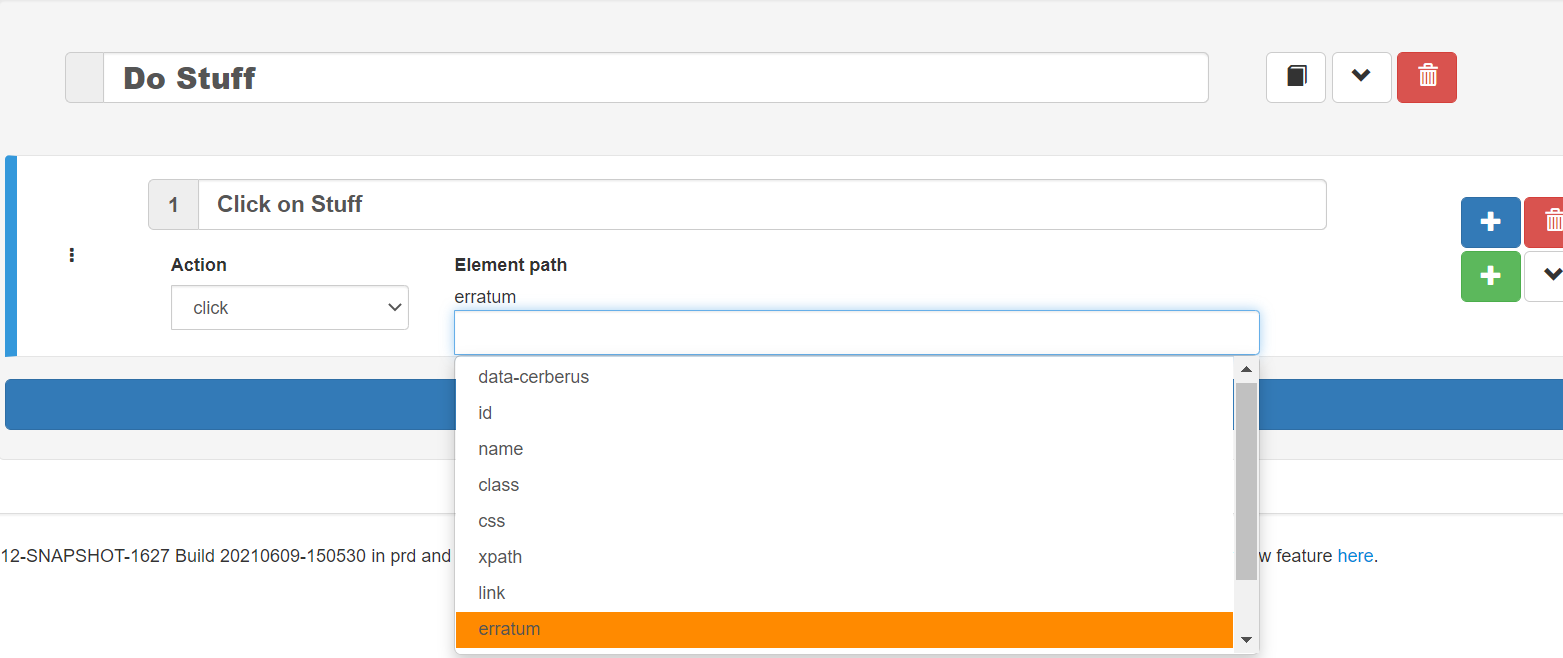
\includegraphics[width=.85\linewidth]{cerberus/explanations/cerberus}
    \caption{A screenshot of the \cerberus web interface to define a test case.}
    \label{fig:cerberus}
\end{figure*}

It appears that these drawbacks are more than a mere inconvenience. 
When first meeting with one of the companies interested in \erratum, we were told that a whole test campaign had to be discarded because the locators included in the considered test cases were constantly breaking during the software development process.

To overcome these problems, \cerberus standardized the use of \textit{data-cerberus} identifiers, which are simple element attributes aimed at uniquely identifying web elements to be used by automated tests.
For example, if developers anticipate that the web testing team needs to interact with a specific application button, they should include such an identifier as follows:
 \begin{lstlisting}
    <button data-cerberus="a_special_button" type="button">Send</button>
\end{lstlisting}

Unfortunately, using such static identifiers entails other challenges, among which:
\begin{compactenum}
    \item it introduces a---probably undesired---tight coupling between the development and testing teams,
    \item if a \texttt{data-cerberus} attribute is missing, the development team should first fix the page under test and then re-deploy the web application, which may take time and several iteration to expose all the required identifiers,
    \item for various reasons, the testing team might not have the possibility to change the source code of the page under test (\emph{e.g.}, proprietary source code), and finally
    \item it forces web developers to anticipate and maintain all these unique identifiers to ensure the absence of identifier collision.
\end{compactenum}

The above observations shared by testing practitioners from \laredoute{} and \cerberus demonstrate that none of the standard locators support a robust execution of their test campaigns.
In the best case, they reported that broken locators causing the failure of a test campaign may require some hours to be fixed.
In the worst case, they even mention that some test campaigns were cancelled and discarded due to the fragility of web locators, thus causing recurrent breakages of test executions and a prohibitive maintenance cost.
Unfortunately, \textit{data-cerberus} identifiers failed to be applied in this specific case, due to the proprietary source code used by the web application under test.
In this context, the integration of \erratum{} in \cerberus{} offers a practical alternative to standard web locators, thus aiming to drastically reduce the cost of broken locators for web testing teams.

\section{Integrating \erratum into \cerberus}\label{sec:integration}
Given the maturity of the \cerberus open-source project, the integration of \erratum{} has been achieved in several steps that we report in this section.
% To help solving the problems described in the previous section, we integrated Erratum to Cerberus.

\subsection{Preliminary Demonstration of \erratum}\label{sec:demo}
Since integrating a solution like \erratum requires a non-negligible amount of work, we decided to start by sharing a demonstration of \erratum's core matching algorithm to encourage testers to assess some of their typical test breakages before starting to integrate.

Given an element $e$ in a DOM $D$, the broken locator problem happens when the locator that located $e \in D$ does not return any results on $D'$.
In this scenario, the key idea of \erratum is to match all elements from $D \to D'$ and use this matching to locate $e \in D'$.
% This matching is done using SFTM. That's why, before integrating Erratum, it was crucial to make sure SFTM yields accurate results on typical web pages used by La Redoute. 

Figure~\ref{fig:demo_app} reports on a screenshot of the demo application.
To use the application, one simply needs to:
\begin{compactenum}[\em i)]
    \item \emph{Input} the URL of 2 web pages to match (\emph{e.g.}, two different product pages or two versions of the same product page),
    \item \emph{Hover} over one of the elements in either page. The corresponding element matched on the other page is automatically highlighted. If none element matches, the input element is highlighted in red,
    \item \emph{Check} that the matched element exists and assess it matches the expected one.
\end{compactenum}

\begin{figure*}[]
    \centering
    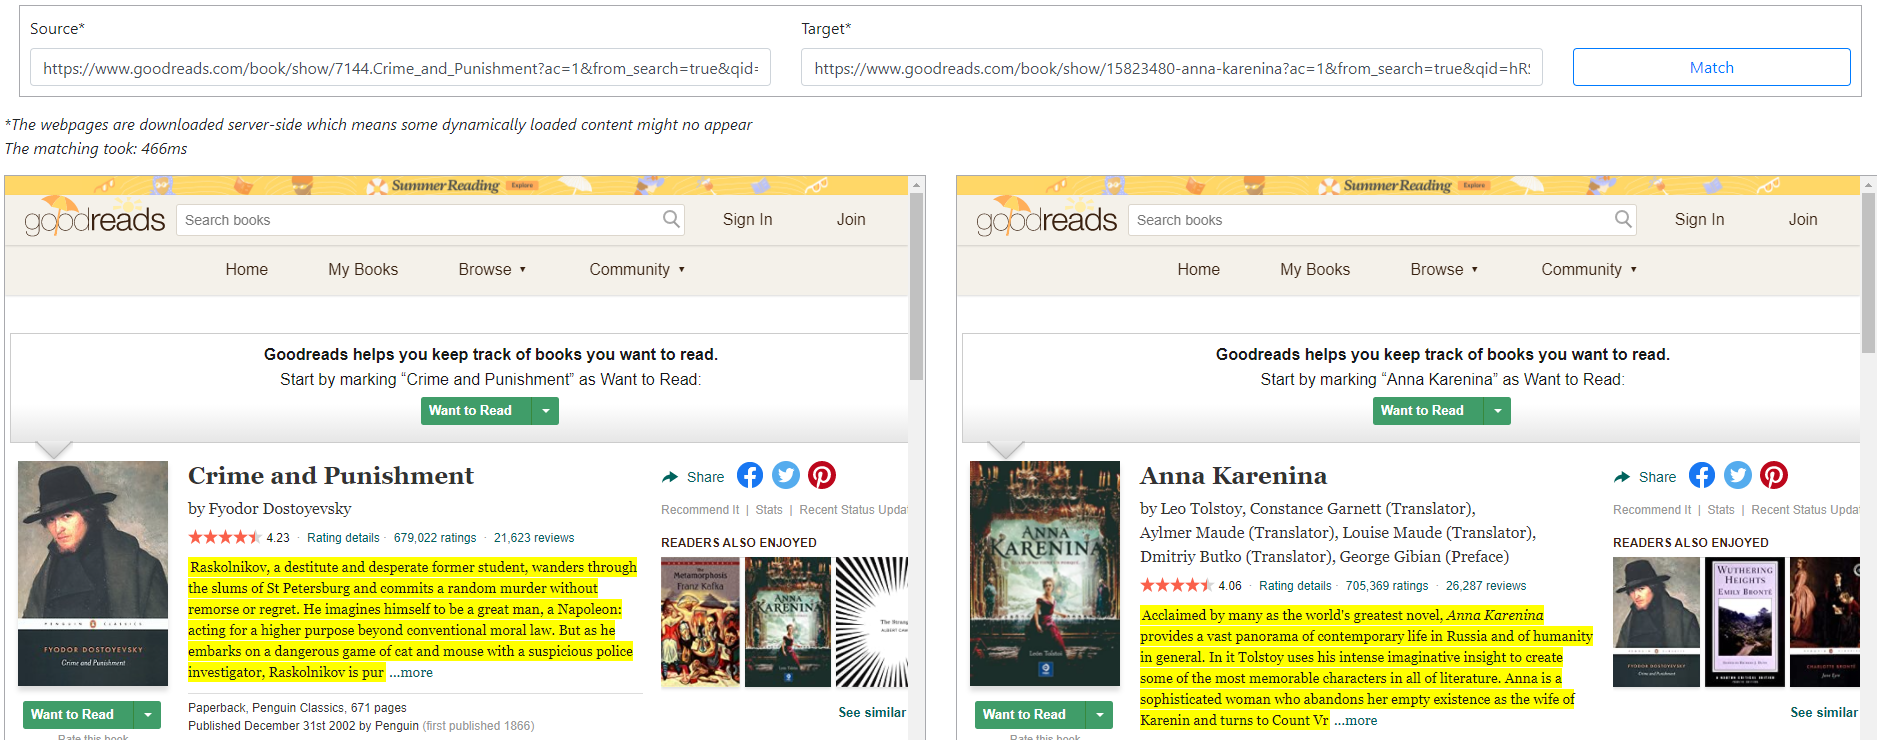
\includegraphics[width=\linewidth]{cerberus/explanations/demo_matching}
    \caption{The demo application developed to test \erratum on real use-cases before starting integration. In this example, the description of a book is hovered on the left-side webpage, which automatically highlights the matched element on the right-side webpage.}
    \label{fig:demo_app}
\end{figure*}

The application also allows users to input HTML files, which allowed to test the matching algorithm on several alternative versions of pages.
This demonstration step constituted a crucial step of the integration process by convincing the \cerberus community of the benefit brought by \erratum with regards to existing support for web locators.
Practitioners quickly understood that the algorithms of \erratum~\cite{brisset2021erratum,brisset2020sftm} could automate most of the situations they were facing during the web testing campaigns.
Furthermore, the fact that \erratum preserved the separation of concerns between the web application and the testing campaign emerged as another convincing argument in favour of \erratum.
Once validated, we moved forward by studying the integration strategies to implement this research results into the open-source platform.

\subsection{Integration Strategies in \cerberus}
Two main strategies were investigated:
\begin{inparaenum}[\em (i)]
\item use \erratum to automatically repair broken locators by fixing automated tests, or
\item use \erratum directly in the \cerberus testing environment, as an alternative way to locate elements.
\end{inparaenum}

The first approach reflects the case study considered in the original \erratum article~\cite{brisset2021erratum}.
The main benefit of this approach is that it can be seamless for the tester: whenever a locator breaks, it is automatically repaired without requiring any action from the tester.
However, integrating such a solution implies some significant changes in the \cerberus architecture.
Indeed, given a locator $l = loc_{e,D}$ that identifies en element $e \in D$, if $l$ breaks on $D'$, then \erratum requires to recover the original page $D$ on which the locator was initially working.
Since the history of pages is not recorded by \cerberus, the repair approach would require some major structural changes to keep track of web application histories.

As a first iteration, we therefore chose the second strategy.
Instead of using \erratum as a locator repair method, we consider its extension as a robust locator method to replace standard locators, like \textit{CSS} or \textit{XPath}, as described in Section~\ref{sec:erratum}.
Interestingly, the existing support for multiple classes of web locators in \cerberus offers a more straightforward hook to integrate \erratum.

\subsection{The \erratum Robust Locators}
To leverage the integration of \erratum in \cerberus, we therefore packaged \erratum as a robust locator.
The key property that differentiates \erratum from other web locators is that \erratum requires the original DOM $D$ on which the element was successfully located.
To build a robust locator with \erratum, we embedded the whole DOM $D$ in the locator---\emph{i.e.}, the \erratum locator of an element $e \in D$ is the pair $(XPath(e), D)$, where $XPath(e)$ is the absolute XPath of $e \in D$.
Figure~\ref{fig:erratum_as_locator} depicts how we extended \erratum to implement to robust locator support in \cerberus:
\begin{compactenum}
    \item from the original page $D$, the tester selects the element to locate $e$,
    \item so far, with XPath:
    \begin{compactenum}
        \item the tester specifies the web locator as an XPath query that she thinks to be robust to select $e \in D$,
        \item during the test execution, the XPath query is executed on the new DOM $D'$. If the locator is not broken, the query evaluation returns $e'$, but if the XPath query fails, then the test scenario is likely considered as broken,
    \end{compactenum}
    \item while, with \erratum{}:
    \begin{compactenum}
        \item the web locator is automatically generated, as a pair $(XPath(e), D)$, where $XPath(e)$ is the absolute XPath of $e$ and $D$ is the full DOM,
        \item during the test execution, \erratum{} first matches all the elements of $D'$ with $D$, and then the resulting matching is used to relocate the matched element $e \in D$ into $e' \in D'$.
    \end{compactenum}
\end{compactenum}

\begin{figure*}[htbp]
    \centering
    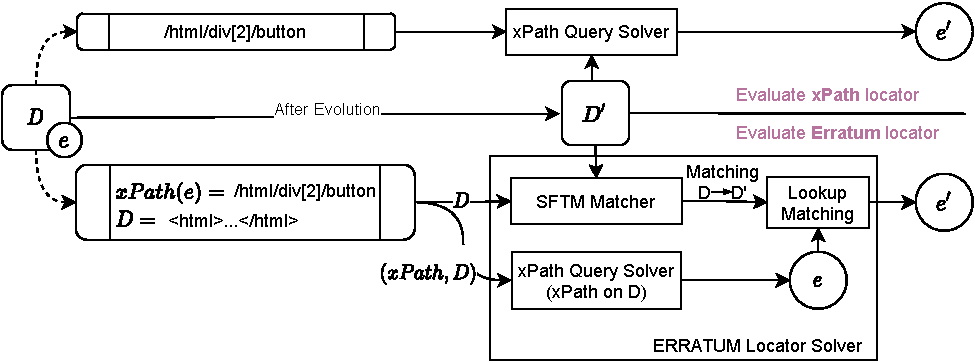
\includegraphics[width=.7\linewidth]{cerberus/explanations/erratum_as_locator}
    \caption{Describing how \erratum is integrated as a robust locator in \cerberus. Both locator types originally locate an element $e \in D$. The figure illustrates the ways \cerberus evaluates XPath or \erratum locators on a new DOM $D'$.}
    \label{fig:erratum_as_locator}
\end{figure*}

% Addressing the integration of \erratum through the robust locator problem rather than locator repair is a subtle pivot that eases the implementation, as it allows \erratum to be included in a similar way to already existing locator methods, like \textit{XPath} or \textit{CSS}.

To allow this integration within \cerberus, we rewrote the generic matching algorithm of \erratum, namely SFTM~\cite{brisset2020sftm}, in a language that can compile to JVM.
The code of the resulting library is open-source\footnote{\url{https://github.com/lssol/sftm\_tree\_matching}} and the library is published in Maven central.\footnote{\url{https://mvnrepository.com/artifact/io.github.amaris/sftm-tree-matching}}
Then, the integration of the \erratum library in the \cerberus platform represents only 127 lines of Java code.\footnote{\url{https://github.com/cerberustesting/cerberus-source/commit/0a70d4cc0d70a797901652fd2b97d501bb7fa511}}

\subsection{Usage}
The usage of the new \erratum locator on Cerberus is very similar to that of other locators.
Given an element $e$ that the tester wants to select on the page $p$, she has to:
\begin{compactenum}
\item select the \erratum locator type on the test case select box (see figure~\ref{fig:cerberus}), and then
\item copy-paste the absolute XPath of $e$ and the whole HTML of $p$ in the input form.
\end{compactenum}
To ease this process, we developed a browser extension allowing to simply click on the targeted element $e$ to copy the required data in the clipboard before pasting it into the input form.

In addition to providing more robust locators, writing test scenario using \erratum along with its extension represents a significant time gain: instead of manually crafting a locator that the tester judges to be robust enough, she simply needs to click on the targeted element. 
It allows the tester to completely ignore the details of how a certain element should be located and instead focus on building the most relevant test scenarios.

\section{Industrial Impact}\label{sec:impact}
Every year, the \laredoute{} web testing team estimated that the locator breakage entailing the failure of their test campaigns induced more than 11\,K\texteuro{} worth of load to their teams.
For industrial projects that evolve quickly, some testing campaigns were even cancelled because of the cost to continuously repair the broken test scripts.
In addition to that, repairing broken locators was considered as a tedious low-value task, which may be harmful to the moral of testers. 
We collected the feedbacks of 2 testers from this team, mainly asking about the biggest pain points faced by the testing team and how a solution like \erratum could help. 
According to the most experience tester we interviewed, most challenges faced by the test team stem from the separation between the development team and the testing team.
The development team is encouraged to push features fast (pressure on quantity), while the testing team's role is to monitor the quality of the released application.
The problem is all the more aggravated by the fragility of the developed test cases: when a new version is released, it takes several days to fix all tests which means that when the tests are ready, the developers are already working on different features.
Hence, using a tool like \erratum helps tightening the feedback loop between the testing team and the development team, thus allowing more intricate collaboration and less friction.

\laredoute{} unfortunately does not conserve a history of failed tests (along with the web page versions), which makes it hard to quantitatively measure the exact percentage of successful relocation of \erratum on their industrial cases.
We collaborated with 5 testing experts working on different campaigns to evaluate \erratum. 
The purpose of this evaluation was mainly to assess if \erratum could be used systematically in place of manually written \textsc{XPath} to locate elements on new tests cases, which would significantly fasten their development and maintenance.
We tried to design evaluation strategies that would not require too much time from the testing experts.
In particular, there were three stages of testing:
\begin{enumerate}
    \item Each tester tested 2 to 3 typical pages from their testing campaigns on the demo described earlier (see section~\ref{sec:demo});
    \item After \erratum was integrated to \cerberus, the \erratum locator type was tested on the same pages within the \cerberus framework;
    \item For two campaigns, each new test case written by the testers was duplicated for a period of one month: one version used an XPath locator and the other version, the \erratum locator.
\end{enumerate}

\begin{table}[]
\centering
\begin{tabular}{l|r|r|}
\cline{2-3}
                                                       & \bf Campaign A & \bf Campaign B \\ \hline
\multicolumn{1}{|l|}{\# Test cases}                        & 16         & 3          \\ \hline
\multicolumn{1}{|l|}{\# Releases}                          & 16         & 2          \\ \hline
\multicolumn{1}{|l|}{\# Locators / test (avg)}             & 18         & 22          \\ \hline
\multicolumn{1}{|l|}{\# Relocations}                       & 4,608       & 132         \\ \hline
\multicolumn{1}{|l|}{{[}XPath{]} \# Locator Failure} & 0          & 1          \\ \hline
\multicolumn{1}{|l|}{{[}\erratum{}{]} \# Locator Failures} & 0          & 0          \\ \hline
\end{tabular}
\caption{Results of the third testing phase that lasted one month.}
\label{table:results}
\end{table}

The evaluation of \erratum attempted to answer two questions:
\begin{enumerate}
\item Is \erratum a viable locator replacement of XPath?
\item Are \erratum locators more robust than manually written XPath locators?
\end{enumerate}

Table~\ref{table:results} presents the results of the third testing phase.
The campaign A applies to an application being completely rewritten, which explains the high frequency of releases.

During a month, there were $4,740$ locator relocations (\# tests $\times$ \# releases $\times$ average \# locators / test) over the two campaigns under study.
For \erratum, none of these relocations failed, while one failed for XPath.

The results thus tend to indicate that \erratum can be safely used as a replacement of manually written {\sc XPaths}.
As for whether \erratum provides more robust locators than manually written XPath, there is still not enough data to conclude. 

Following the evaluation, \laredoute{} now adopted \erratum as the preferred locator method, along with \texttt{data-cerberus} attributes, and have not yet reported any relocation failure at the time of writing this paper.
Beyond the collaboration with \laredoute, we believe that these promising results will benefit to the wider \cerberus community.

\section{Perspectives}\label{sec:perspectives}
\paragraph{Visual integration}
considering the above \erratum web extension, the tester no longer needs to analyze the HTML source code and manually assemble a robust locator.
It means that, theoretically, \cerberus could integrate a fully visual locator selection approach where
\begin{inparaenum}[\em (i)]
    \item the tester fills in the web application URL,
    \item the page opens in an iframe,
    \item the tester selects the target element,
    \item the \erratum locator is automatically generated.
\end{inparaenum}
This process was originally considered, however, it would not be usable in more complex situations where some pages are not directly accessible from a given URL (\emph{e.g.}, a page that requires to login first).

\paragraph{Mobile testing}
the web testing teams in the \laredoute{} company also use \cerberus to automate tests from mobile devices.
Web pages are described using HTML and Android views are written in XML.
While HTML and XML are very similar and our tree matching library theoretically allows \erratum to match any kind of tree (and not only HTML trees), some technical adjustments still need to be completed to include XML trees in \cerberus.
Furthermore, the robustness of \erratum's locators to typical Android XML view mutations still need to be assessed, as they may differ from typical HTML mutations.

\section{Conclusion}\label{sec:conclusion}
Web locators remain a fragile keystone of automated test suites executed by modern test platforms.
Whenever a locator fails to locate a web element in a test suite, it directly impacts the whole test campaign and impose some additional maintenance tasks to the web testing team.

In this paper, we described how we extended and successfully integrated the locator repair solution \erratum into \cerberus, a widely used open source test-automation solution.
In particular, we reported on the development of a robust locator based on \erratum that eases the pain of web testers, by saving time and reducing the cost of test campaigns.

\chapter{Appstract}\label{chap:appstract}
\section{Introduction}\label{sec:introduction}
Web applications are often perceived by end-users as online systems exposing a limited set of views, concepts, and related actions.
% As humans, we see a web application as composed of a relatively limited amount of views exposing a limited amount of potential actions. 
From a user perspective, an online shop---like Amazon---mainly offers to search and list products, while clicking on a given product brings us to its details view. 
From a machine perspective, like a bot, navigating the same web application will be perceived as crawling thousands of unique pages, exposing unrelated content and seemingly unique actions.

This inability for a machine to understand the navigation model of a web application, like a user intuitively does, makes it very hard to automate interactions with web applications.
Typically, research topics benefiting from more intuitive navigation include:
\begin{inparaenum}[\it (a)]
    \item \emph{web data mining} to automatically extract, de-noise, and structure data from web pages,
    \item \emph{web testing} to generate, maintain, repair, and augment tests on web applications, and
    \item \emph{web analytics} to report on how users interact with the web application.
\end{inparaenum}

While there is a considerable amount of existing literature, notably in the fields of data mining~\cite{Zhai2005WebAlignment, ArasuExtractingPages, Crescenzi2001RoadRunner:Sites, Sarawagi1996InformationExtraction, ChaudhariTemplatePages, MiaoExtractingClustering}, most of existing works are highly specific and do not provide adequate insights to build an application-wide understanding of a navigation model.

In particular, state-of-the-art approaches focus on either extracting data within a page (so-called, \emph{intra-page} extraction) or across two pages (\emph{inter-page} extractions). 

For example, Miao~\textit{et~al.}~\cite{MiaoExtractingClustering} clusters full tag paths---\emph{i.e.}, \texttt{/html/bo\-dy/div[2]/div[1]/span}---to detect repeating occurrences of a template within a page.
This allows their approach to extract what are usually called \emph{records} in a web page (\emph{e.g.}, a single product card in a product list).
This is an example of what we categorize as \emph{intra-page abstraction}.

\emph{Inter-page abstraction} solutions usually try to detect templates of a webpage or to learn a wrapper by studying two different instances of the same template.
That is what is done by the state-of-the-art algorithms, like EXALG~\cite{ArasuExtractingPages} and \textsc{RoadRunner}~\cite{Crescenzi2001RoadRunner:Sites}.
However, none of these approaches provide any insight to take into account the intra-page variability.

In this chapter, we thus propose an unsupervised approach to infer the navigation model of a whole web application that we call an \textit{appstraction}.
The \textit{appstraction} of a web application aims at delivering actionable insights: it allows a machine to understand application states (\emph{e.g.}, product pages, blog page), as well as elements within states (\emph{e.g.}, product title, price), hence guiding the information extraction process, as well as identifying relevant navigation actions.
The \textit{appstraction} process aims to abstract away the natural variability of web pages into a canonical model built as a compact tree of \emph{template pages} and \emph{template elements}.
Our unsupervised approach assumes that even web applications with billions of pages will build on a limited set of template pages, thus making it possible to infer these generative templates from a dataset of visited pages.
To achieve this, our approach---named \textsc{Appstract}---builds on three stages:
\begin{inparaenum}
    \item \textit{web page clustering} to group instances of related web pages,
    \item \textit{intra-page abstraction} to extract repeating patterns within each cluster of pages, and
    \item \textit{inter-page abstraction} to capture repeating patterns across clusters.
\end{inparaenum}

We empirically demonstrate that our \emph{appstraction} succeeds to generate application-wide locators that can be used to support semantic guidance across multiple pages of any web application.
\textbf{MORE TO BE SAID ON THE DEMONSTRATION}.

The remainder of this chapter is therefore organized as follows.
Section~\ref{sec:related} introduces the required background and related works in this area.
Section~\ref{sec:appstract} presents the design and implementation of \textsc{Appstract}, while Section~\ref{sec:evaluation} reports on an evaluation of the perceived accuracy of \textsc{Appstract}.
Finally, Section~\ref{sec:conclusion} concludes.

\section{Background \& Related Works}\label{sec:related}
In this section, we present several studies across different research fields that offer partial solutions to the general problem of web application abstraction inference. 
Throughout this chapter, we consider a subset of the Amazon web application as a running example.
In particular, we focus on two related page templates: the product details and product list pages (cf. Figure~\ref{fig:amazon}).

\begin{figure*}[ht]
  \centering
  \begin{subfigure}{.35\textwidth}
    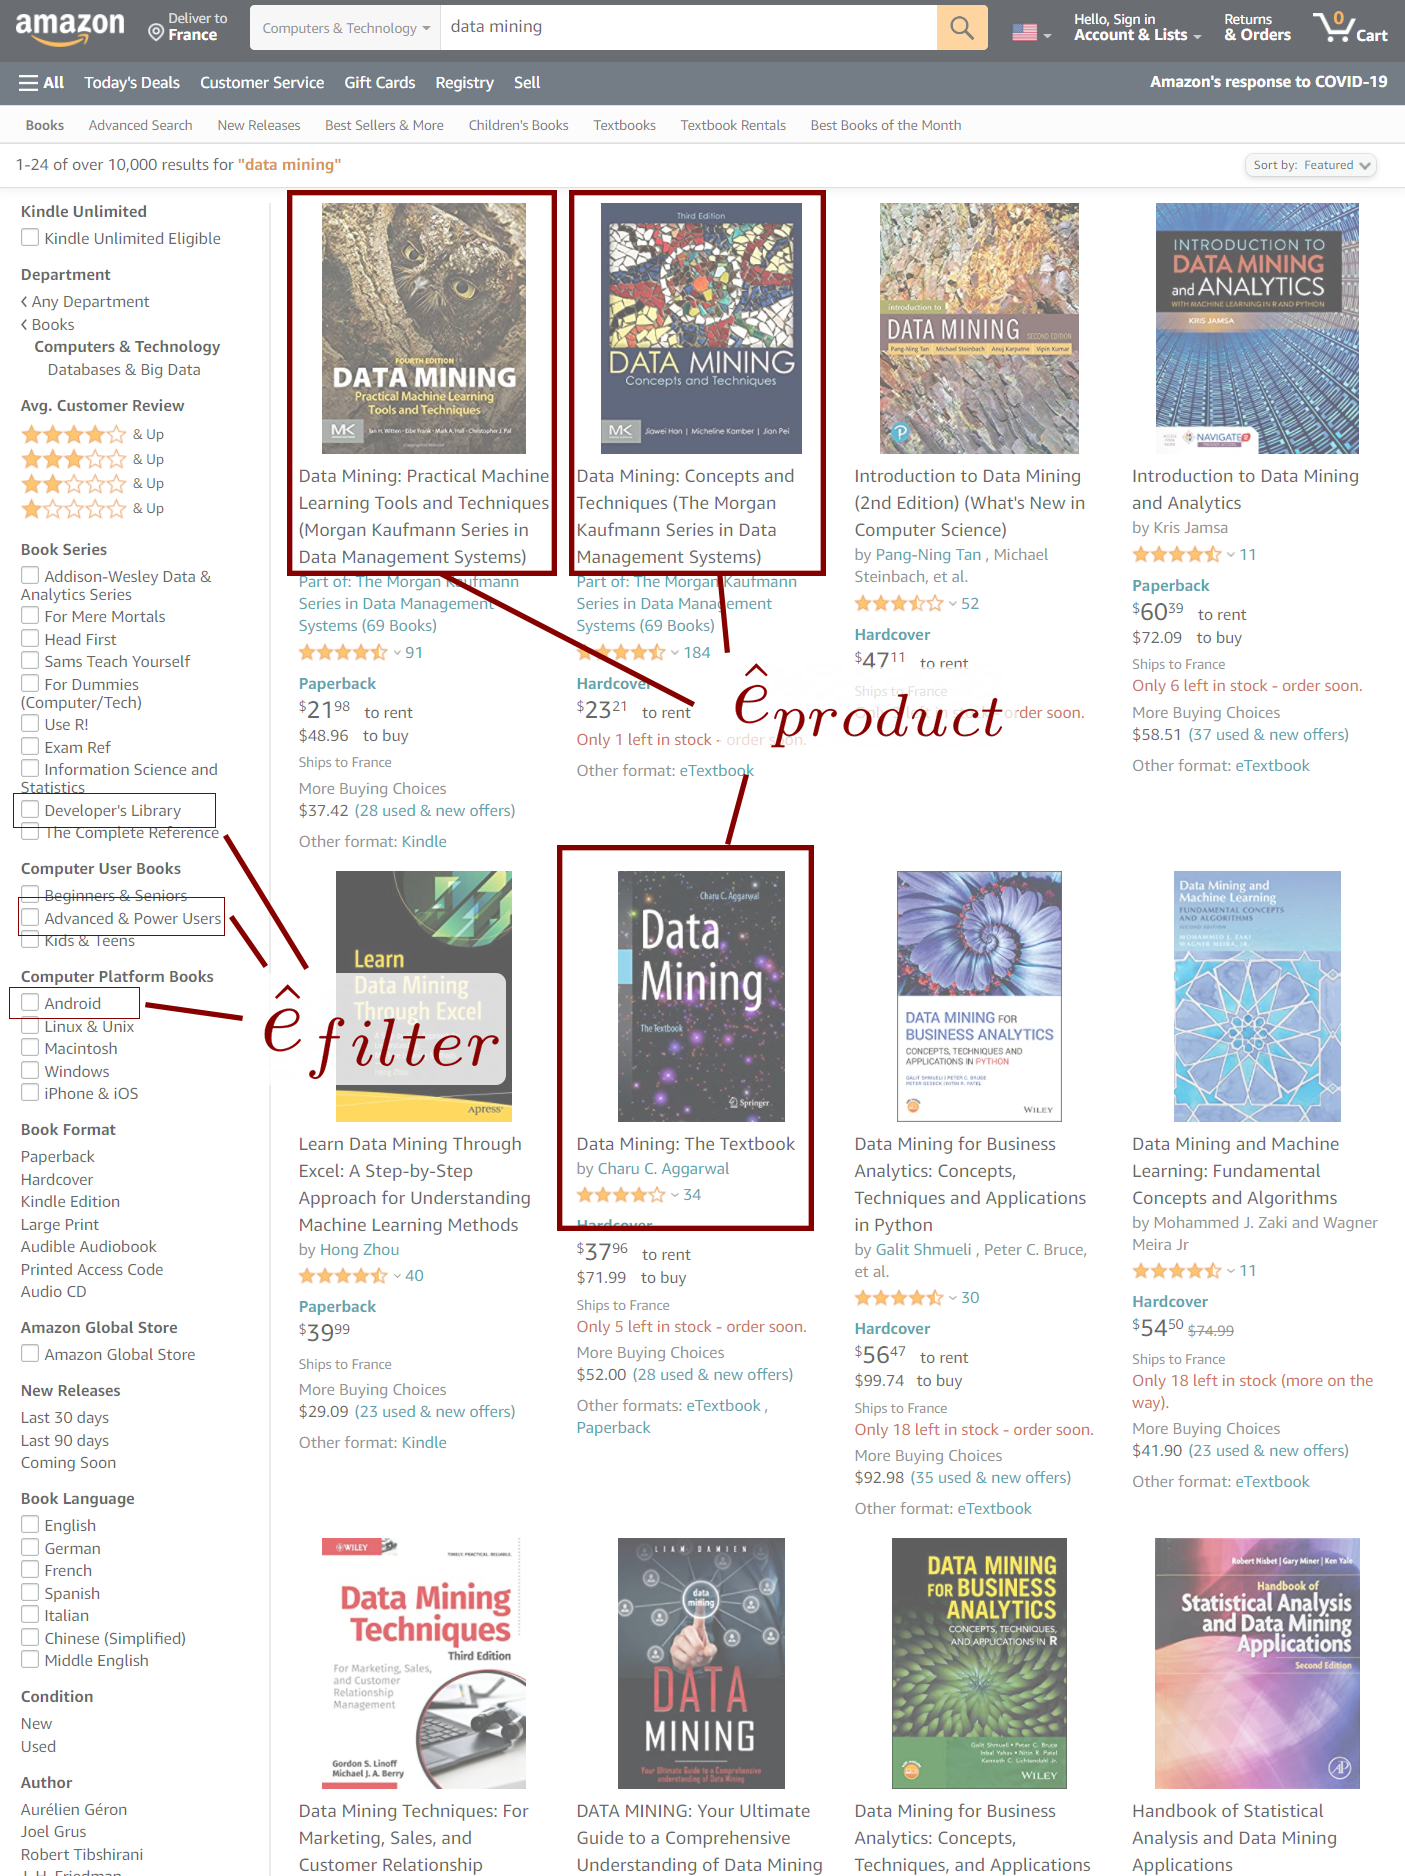
\includegraphics[width=\linewidth]{appstract/amazon_a.png}
    \caption{Sample page from cluster $list$.}
    \label{fig:amazon_a}
  \end{subfigure}
  \hspace{.1\textwidth}
  \begin{subfigure}{.35\textwidth}
    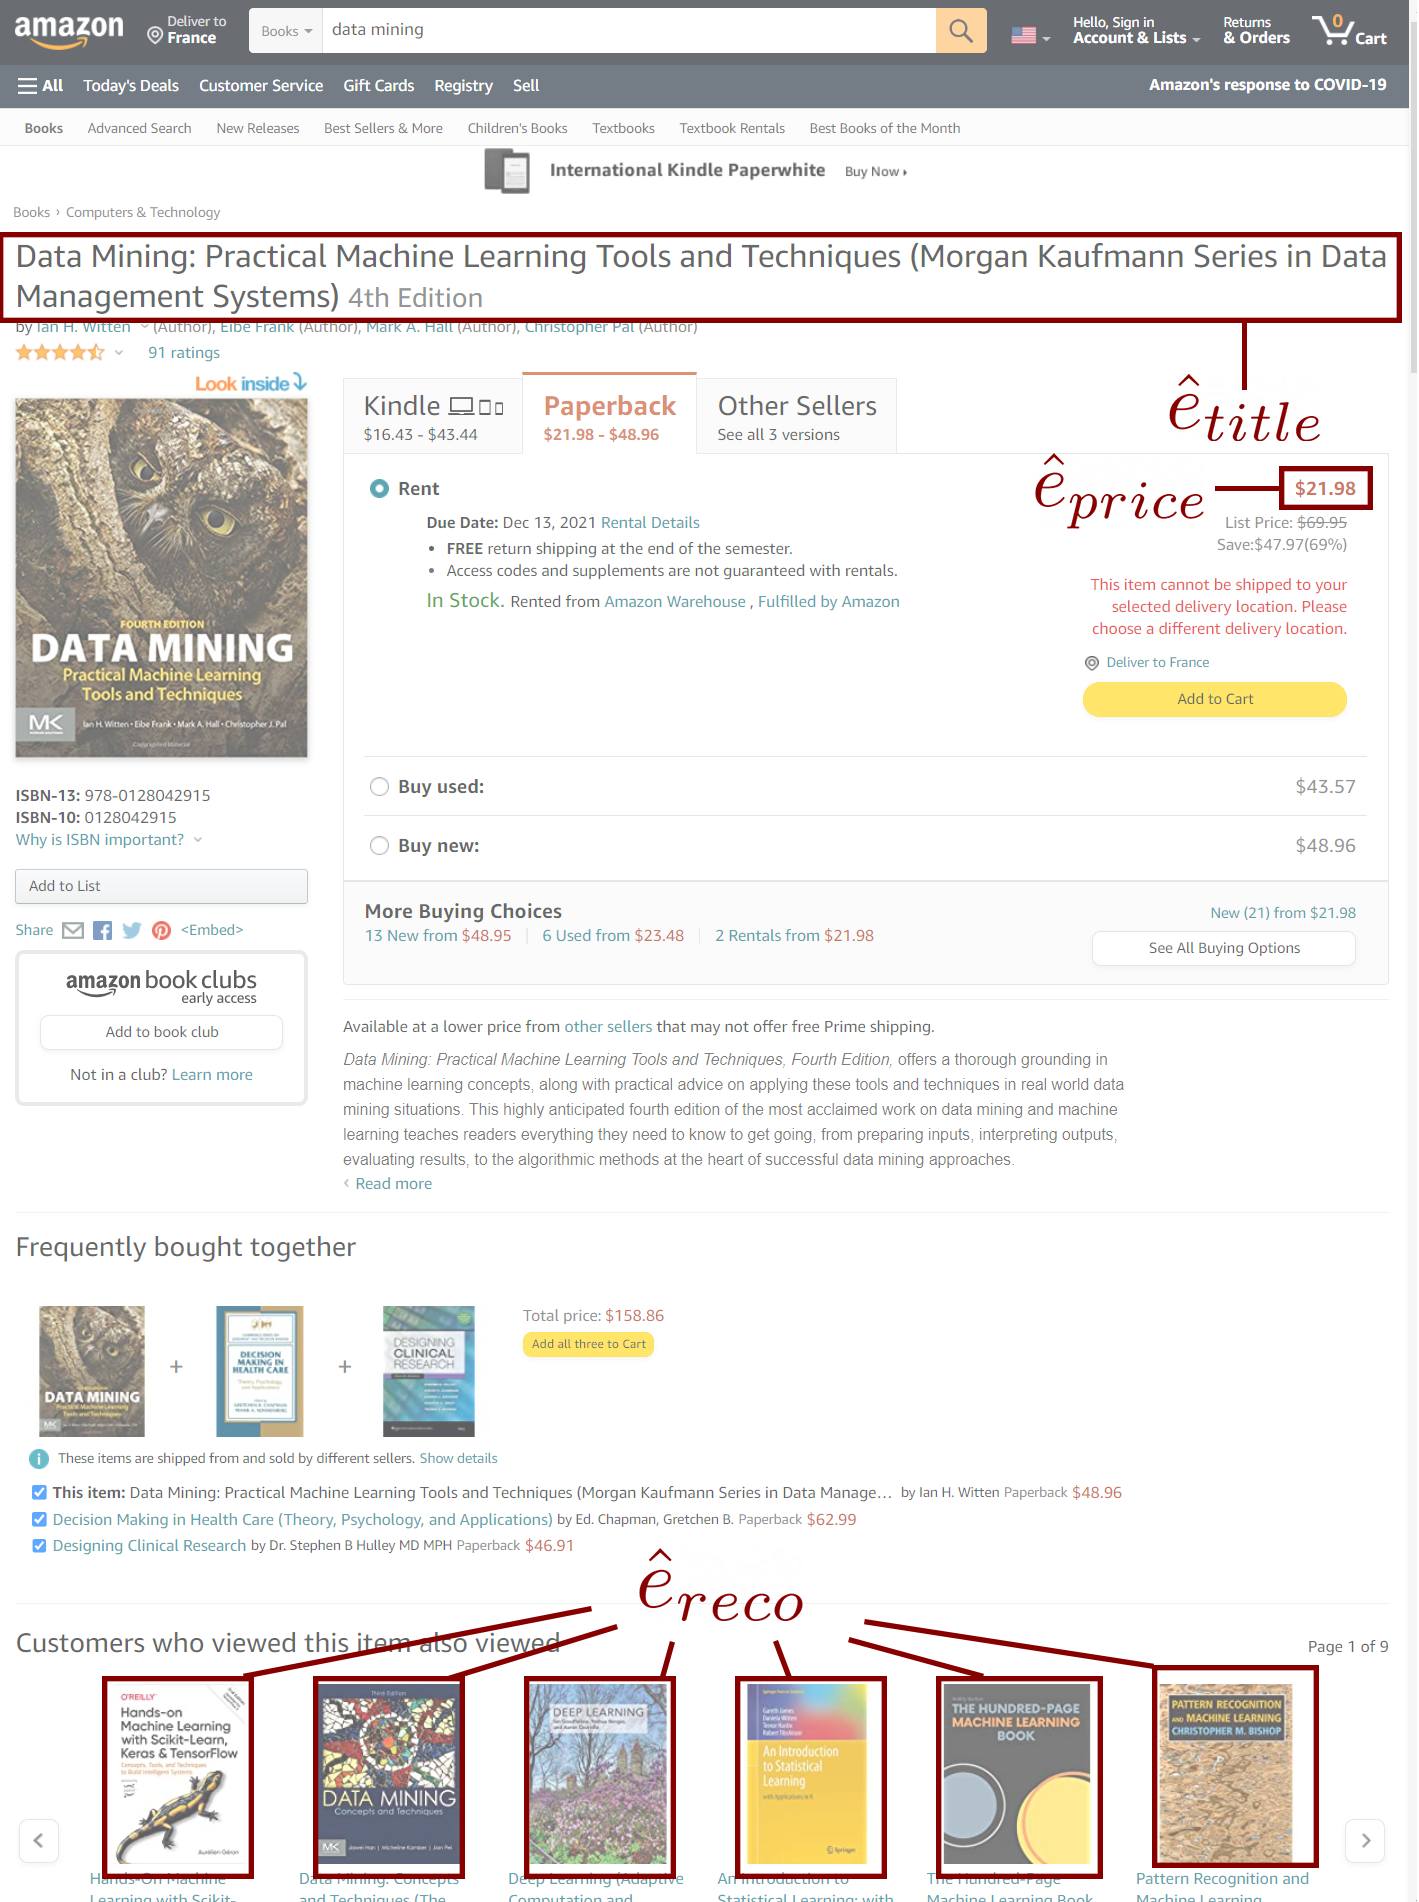
\includegraphics[width=\linewidth]{appstract/amazon_b.png}
    \caption{Sample page from cluster $product$.}
    \label{fig:amazon_b}
  \end{subfigure}
  \caption{Screenshots illustrating some elements $\hat{e}_{\lambda}$ included in the template pages $\hat{p}_{list}$ and $\hat{p}_{product}$ of 2 distinct clusters.}
  \label{fig:amazon}
\end{figure*}

\subsection{Data Extraction}
The role of a web page is mainly to \emph{present} a subset of the information it has access to in a certain way.
All data extraction solutions attempt to separate the information from its presentation---\emph{i.e.}, the template.
The process of data extraction is thus a form of abstraction of an application: instead of viewing the different pages as a multitude of unrelated blobs of HTML, the application is seen as a limited set of templates that presents various information in a consistent way.
The process of information extraction is thus closely related to our \emph{appstraction} objectives and our approach is highly inspired by the ideas behind data extraction. 

Following the classification made by a survey on data extraction~\cite{Chang2006ASystems}, most existing literature on data extraction can be classified according to the levels of supervision needed to extract the data:
\begin{compactitem}
    \item \emph{(semi-)supervised approaches} where the user inputs more or less detailed directions to describe to how to extract data~\cite{Barish2000TheaterLoc:Applications,Huang2000ExtractingWEB,Levy1996QueryingDescriptions,Muslea1999ExtractionSurvey,Gottlob2004Logic-basedExtraction,Gottlob2004MonadicExtraction,Hsu1998GeneratingWeb},
    \item \emph{unsupervised approaches} where data is automatically extracted by analysing recurring patterns~\cite{Crescenzi2001RoadRunner:Sites,ArasuExtractingPages,Liu2003MiningPages,Wang2002WrapperDiscovery,Wang2002WrapperDiscovery}.
\end{compactitem}

Supervised approaches are usually qualified as "wrapper-based".
The idea of wrapper-based data extraction is to consider the set of web pages containing the data to extract as an unstructured (or semi-structured) database and build a query language (and its query engine) to query the desired data.

In this chapter, we focus solely on \emph{unsupervised approaches}.
These approaches rely on the assumption that, even though there is a lot of different pieces of information exposed by an application, the same type of information will always be structured in the same way.
For example, on the product list page of an online shop, each product will be structured in a similar fashion (\emph{e.g.}, product name, price, description).
In this context, we distinguish two families of unsupervised approaches: \emph{intra-page} and \emph{inter-page} data extraction.
One should note that \emph{intra-page} data extraction is usually referred as \emph{record extraction}~\cite{Chang2006ASystems,DeReis2004AutomaticDistance}. 

\emph{Intra-page data extraction} refers to the extraction of data within a page.
For example, in the case of the Amazon page presented in Figure~\ref{fig:amazon_a}, an intra-page data extraction solution, such as MDR~\cite{Liu2003MiningPages}, relies on the topology of the DOM tree and string matching to detect data regions $\hat{e}_{product}$ within a single page.
As it is always the case when attempting to extract data in an unsupervised way, MDR can only detect data regions if at least two of these regions are present on the page.
This is a necessary condition since all unsupervised algorithm must rely on some kind of pattern discovery to detect data regions.

\emph{Inter-page data extraction} refers to the extraction of data across several pages.
In particular, all existing algorithms apply to pages that are assumed to belong to the same template (\emph{e.g.}, two Amazon product pages).
The idea is then to use the similarity between the two pages to understand what is common and what has changed between the two pages.
The parts that changed are then assumed to be data, while the common part has to do with its presentation (\emph{template}).
In order to compare these pages, one solution~\cite{DeReis2004AutomaticDistance} uses a modified version of the most popular general tree matching solution: \emph{tree edit distance}.
In the inter-page abstraction part of our approach, we also use a tree matching solution but not the same one.

The challenge of data extraction presented above is very similar to that of our \emph{appstraction} objective. However, it differs in a few important points:
\begin{enumerate}
    \item while data extraction focuses on extracting data, we try to abstract any kind of variability.
    For example, in Figure~\ref{fig:amazon_a}, a data extraction solution should not attempt to extract the $\hat{e}_{filter}$ template elements, as they do not represent data.
    \item several data extraction studies are focused on how to infer a schema of the extracted data (\emph{e.g.}, relational schema~\cite{ArasuExtractingPages,NestorovExtractingData})), which we are not interested to do in the context of \emph{appstraction}, and
    \item most importantly, to the best of our knowledge, no previous work has attempted to extract data throughout a whole web application (combining both inter-page and inter-page abstraction).
\end{enumerate}

\subsection{Web Testing}
Web testing covers a large body of research that encompasses various themes, such as test generation, test coverage, or test robustness.
We claim that, essentially, the main challenge of web testing comes from the lack of abstract understanding of the application under study and most works in this field have to resort to ingenious ideas to compensate for this lack of abstract model.

\paragraph{Test Robustness}
One of the main challenges of web testing encountered by the industry is test breakage: tests written for a given version of a web application break when the application evolves.
For example, let us consider a testing script that applies to a web page $D$.
One part of the script instructs to click on a given button $e$ in the page $D$.
To locate $e$, scripts usually use xPath or CSS selector to build what is called a \emph{locator} $l_e$. 
Breakage can then happen when a new version $D'$ of the page $D$ is published.
Most of these breakage are locator based~\cite{Hammoudi2016WhyBreak}: the locator $l_e$ that successfully located $e$ on $D$ does not locate the matching element $e'$ in $D'$. 
To solve this problem, some attempt to automatically generate more robust locators relying on the structure to the tree~\cite{Leotta2016spanLocators, Leotta2021Sidereal:Testing, Yandrapally2014RobustClues, Bajaj2016SynthesizingLocators} while other works offered solutions to repair broken locators~\ref{chap:erratum}.

In particular, The \textsc{Erratum} approach~\ref{chap:erratum} achieves high accuracy specifically thanks to a more holistic stance: instead of looking at individual locators independently, the approach considers the page as a whole using a similar technique to the \emph{inter-page abstraction} part of our \emph{appstraction}.

The "locator" problem is a more specific instance of the web application abstraction: the breakage happen because when a machine sees a multitude of different pages (\emph{e.g.}, different versions), a human perceives a single page template with slight differences and thus comes to expect the locators on $D$ should naturally work on $D'$. 

In the present work, we go beyond \textsc{Erratum}~\ref{chap:erratum} on the generalization scale and create "locators" that are valid through all pages of a web application.

\paragraph{Test Generation}
Automatic test generation is a domain of research that studies different approaches to automatically generate tests. Most test generation techniques rely on an abstraction of the application called a navigational model. A navigational model of a web application describes the different states an application can be in and the transitions between them~\cite{mesbah2009invariant}.

There exists many approaches to take advantage of this navigational model. The goal of these techniques is to generate the minimum amount of tests that covers a maximum of the application's behavior given a navigation model~\cite{leveau2022fostering, mesbah2009invariant, yuan2007using, biagiola2019diversity}

We are particularly interested in the generation of the underlying navigational model.
The navigational model can be written manually, for example, Leveau and al.~\cite{leveau2022fostering} developed a whole Domain Specific Language to describe this navigational model. 
It can also be generated. The only approach we managed to find that generates a navigational model is APOGEN~\cite{stocco2017apogen}. APOGEN is quite close in spirit to our APPSTRACT solution. The idea of APOGEN is not originally to create a navigational model, but to create \textit{page objects}. However, it has been used as a way to generate a navigational model~\cite{biagiola2019diversity}. APOGEN crawls, clusters and then analyses the different clusters of web application to generate page objects. The main difference with our approach is that APOGEN is heavily based on the analysis of links to understand how different pages interact with one another and most importantly, it does not include any \textit{intra-page abstraction}.

\subsection{Web Analytics}
Web analytics deals with the analysis of the user behavior on a given web application.
A lot of studies have been published on the subject since the popularisation of the web. However, most works are applied on controlled environments where the ability to automatically infer an abstract model of an application is not needed. For example, some research focus solely on mouse movements~\cite{guo2008exploring, yamauchi2013mouse} or focus on a given search engine and try to analyse behavior to optimize search results~\cite{agichtein2006learning, agichtein2006improving}.
Research that do rely on a certain model of an application usually use an \textit{url-based} model. While the first research works on the subject, at the beginning of the web, could use simple logs of visited urls~\cite{gunduz2003web, mobasher2001effective, sarukkai2000link}, modern web applications are generally much more complex with virtually unlimited amounts of urls dynamically generated making it hard to reason about unprocessed logs of visited urls.
To tackle this challenge, recent work on web browsing behavior use a variety of techniques to encode url like Recurrent neural network~\cite{Ou2021ModelingSide} so that several strictly different urls that refer to the same template page will have similar encodings. While using url-based encoding to create an abstract model of a web application can help abstracting relationship \textit{between} pages (given that they contain enough information which depends on the application), it will not provide the \textit{intra-page} abstraction that we need to obtain meaningful encodings within pages.

\section{Appstract}\label{sec:appstract}
\subsection{Abstracting a Web Application}
This section starts by defining the notions of \emph{application} and \emph{application abstraction} we assume, before discussing the challenges of inferring such defined abstractions.

\begin{defn}[\em Application]
A web application $A$ is a set of web pages $\{p \in A\}$, where every page $p$ is captured by a \emph{Document Object Model} (DOM).
\end{defn}

The number of web pages $\|A\|$ can be very high and keep rising with time (\emph{e.g.}, Amazon products or blog posts).
In addition, we consider that any mutation of a web page (even if the URL does not change) is considered as a new page.
Obviously, from a human perspective, a web application is much more than a collection of pages (\emph{e.g.}, the pages are linked, the application has different features usable by different users), but we choose to take the perspective of a machine, for which an application is perceived as a set of visited web pages.
% 
As a DOM of a page $p$ is a tree, we represent it as a tuple $\langle N(p), par \rangle$ where $N(p)$ is the set of elements (or nodes) in $p$ and $par: N(p) \to N(p)$ is the parent function that associates a DOM node with its parent.
To lighten the notations, we write $e \in p$ to describe an element $e$ in a page $p$, instead of writing $e \in N(p)$.

\begin{defn}[\em Application abstraction]
The abstraction of a web application $A$ is a tuple $\langle\hat{A}, T_{\hat{A}}\rangle$ where \emph{i)} $\hat{A}$ is the set of template pages and each page $\hat{p} \in \hat{A}$ contains template elements $\hat{e} \in \hat{p}$ and \emph{ii)}:
\begin{align}
  \label{eq:1}
  \begin{split}
    \forall p \in A, T_{\hat{A}}(p) & = \langle\hat{p}, T_{\hat{p}}\rangle \\
    \text{and } \forall e \in p, T_{\hat{p}}(e) & = \langle\hat{e}\rangle
  \end{split}
\end{align}\end{defn}

In other words, the abstraction of a web application $A$ is a set of template pages (\emph{e.g.}, product page, list page) and a function that allows to map any page from $A$ to its corresponding template, and every element within the page to the corresponding element in the template page.
This mapping is completed by two functions:
\begin{enumerate}
\item $T_{\hat{A}}: A \to \hat{A}$ is the template function that takes any page $p \in A$ and returns the matched \emph{template page} $\hat{p} \in \hat{A}$, and
\item $T_{\hat{p}}: N(p) \to N(\hat{p})$ is a function that takes any element $e \in p$ and returns the matched element in the template $\hat{e} \in \hat{p}$.
\end{enumerate}

Additionally, we also use:
\begin{itemize}
  \item $T^{-1}_{\hat{A}}(\hat{p}) \subset A$ as the set of pages $p \in A$, such that $T_{\hat{A}}(p) = \hat{p}$, and 
  \item $T^{-1}_{\hat{p}}$ as the inverse function of $T_{\hat{p}}$.
\end{itemize}
These notations allow us to easily refer to the instance pages/elements of a given template page/element.

Figure~\ref{fig:amazon} depicts a theoretical application of the appstraction to 2 web pages crawled from Amazon.
For each related clusters of similar web pages, the $T_{\hat{A}}$ function will return either template page $\hat{p}_{list}$ or $\hat{p}_{product}$.
Then, for each clustered web page, each web element can be mapped to its corresponding template element (\emph{e.g.}, $\hat{e}_{title}$, $\hat{e}_{product}$) using the $T_{\hat{p}}$ function.

Please note that our \emph{appstraction} process does not intend to label template pages or elements.
Thus, our references to $\hat{p}_{list}$ or $\hat{e}_{product}$ should be understood as a \emph{global unique identifier} (GUID) capturing a class of pages and elements within and across clusters.
% , it is solely for pedagogical purpose: while a good appstraction of the application would be able to map all instances of $\hat{e}_{product}$ to the same template element, we do not provide any solution to infer the label ("product" in this case) of this template element.

\subsection{Building an Abstraction}

\begin{figure*}[ht]
  \centering
  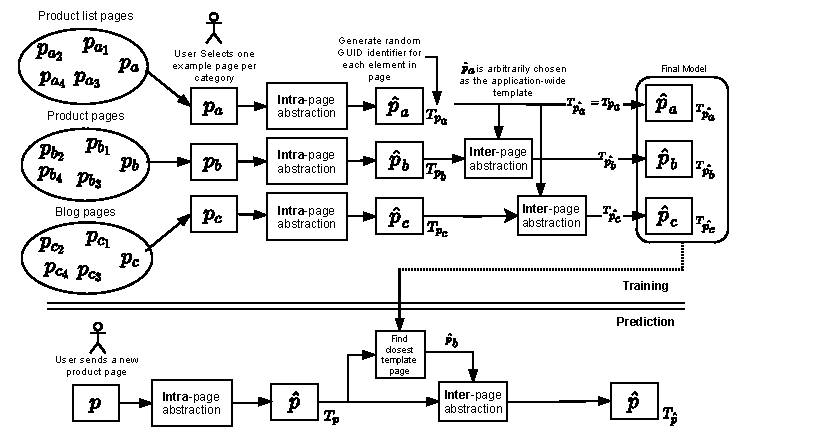
\includegraphics[width=0.8\linewidth]{appstract/explanations/appstract_overview}
  \caption{Overview of the two stages of the \emph{appstraction} process: \emph{learning} and \emph{prediction}. The identifier map of $p$ noted $T_p$ associates an identifier to each element of $p$. The identifiers are first randomly generated, then merged to existing maps during inter-page abstraction. The prediction phase produces an identifier map $T_{\hat{p}}$ in which each original element of $p$ is associated to an application-wide identifier.}
  \label{fig:appstract_overview}
\end{figure*}

To abstract the web page $p$ into its \emph{appstraction} $A_p$, we operate at two levels:
\begin{enumerate}
  \item \textit{intra-page abstraction} to extract repeating patterns of elements within a cluster of web pages, and
  \item \textit{inter-page abstraction} to group repeating patterns of elements across template pages.
\end{enumerate}

This bi-level abstraction process combines two steps: \emph{learning} and \emph{prediction}, as depicted in Figure~\ref{fig:appstract_overview}.
% There are two stages to the overall appstraction process: \emph{training} and \emph{prediction}.
% Figure~\ref{fig:appstract_overview} describes how both stages contribute to build an application abstraction.
% 
In this section, we first overview the abstraction process by considering intra- and inter-page abstractions as black boxes. 
In the following sections, we provide an in-depth description of individual level abstraction techniques.

\paragraph{Learning}
The objective of the learning phase is to build a model of the application that will deliver accurate predictions.
The upper part of Figure~\ref{fig:appstract_overview} describes how intra- and inter-page abstractions are used to build this model.

Before any abstraction, the application is perceived as a set of related pages.
The first step is thus to organise these pages into clusters, each cluster representing a template page (\emph{e.g.}, product page).
In order to do this, any clustering algorithm could be used and, in this chapter, we consider the clustering part as out of scope as we focus on the actual abstraction process.
The learning approach thus starts with the user picking one example page per template.

Each template page goes through intra-page abstraction.
The intra-page abstraction takes a DOM tree $p$ as input and returns a \textit{template} as output.
A \textit{template} is a tuple $t = \langle \hat{p}, T_p \rangle$ where $T_p$ is the identifier map that maps every element from the original tree $p$ to a global identifier. After the intra-page abstraction, $\hat{p}$ typically contains much less elements than $p$ since all repeated patterns have been abstracted away.
The $T_p$ map is a way to keep track of the elements in the original page $p$ after abstraction.
For example, in Figure~\ref{fig:intra} illustrating intra-page abstraction, the identifier map would contain 11 entries, one for each original element in $p$ and 5 distinct values corresponding to the five distinct nodes of $\hat{p}$.

In practice, the values of $T_p$ are \emph{Global Unique Identifiers} (GUID).
Before starting the abstraction process, we transform the page $p$ into a \textit{template} tuple, where the identifier mapping maps every node to a randomly generated GUID.
Each abstraction step will thus transform the input tree and update the associated identifier map.

Once each page has been abstracted at the intra-page granularity, we build a model allowing to achieve two aspects of inter-page abstraction:
\begin{itemize}
    \item \textit{Template abstraction:} same elements within different instances of a template must have the same identifiers (\emph{e.g.}, title of a product on different product pages)
    \item \textit{Cross-template abstraction:} same elements within different pages (regardless of templates) should have the same identifiers. (\emph{e.g.}, menu link that appears on all template pages)
\end{itemize}

To achieve cross-template abstraction, we arbitrarily select one template to represent the whole application ($\langle \hat{p}_a, T_{p_a} \rangle$ in Figure~\ref{fig:appstract_overview}) we call this template the \textit{mother template}.
All other template pages are then inter-page abstracted against the mother template. 
The inter-page abstraction function takes two templates: a reference template and a query template. It then returns one template in which the values of the identifier map have been updated to match the reference template.

The final model is obtained after applying intra-page abstraction between the mother template and all other pages.
The final model is simply a set of $n$ templates where each template is a tuple $\langle \hat{p}, T_{p} \rangle$.

\paragraph{Prediction}
During the prediction phase described in the bottom part of Figure~\ref{fig:appstract_overview}, the user sends a previously unseen page and \textsc{Appstract} returns the mapping between each element $e$ of the page and the \textit{id} of the associated template element $\hat{e}$.

To do so, \textsc{Appstract} first applies intra-page abstraction to create an abstracted DOM tree $\hat{p}$, then applies the tree matching algorithm at the core of the inter-page abstraction between $\hat{p}$ and all templates in the model.
The template page from the model that matches best with $\hat{p}$ is retained (\emph{e.g.}, $\hat{p_b}$ in Figure~\ref{fig:appstract_overview}).

The matching between $\hat{p}$ and the corresponding template is then used to compute the final mapping $T_{\hat{p}}$.

Overall, the user sent a page and received the mapping between each element of the page and the corresponding template element in the corresponding template page.

In the following sections, we describe both intra-page abstraction and inter-page abstraction in more details.

\subsection{Intra-Page Abstraction}

\begin{figure*}[ht]
  \centering
  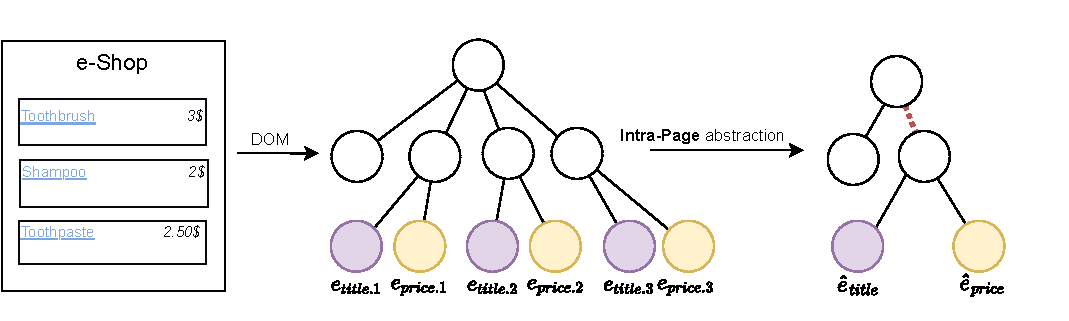
\includegraphics[width=0.8\linewidth]{appstract/explanations/intra}
  \caption{Illustration of Intra-Page abstraction. DOM leaves at the end of repeating branches are tagged and then recursively merged.}
  \label{fig:intra}
\end{figure*}

Intra-page abstraction relies on the detection of repeating patterns within a page. 

Building the intra-page abstraction corresponds to creating the $T_e$ function defined above.
The intra-page abstraction deals with a single page: given an input page $p$, we want to build a template page $\hat{p}$ and a function $T_e$ that maps all the elements $e \in p$  to their corresponding elements $\hat{e} \in \hat{p}$
Overall, the Intra-Page abstraction is done in three steps:
\begin{enumerate}
  \item \emph{Leaf clustering} clusters repeating DOM leaves together,
  \item \emph{Node tagging} propagates information about leaf-clusters in all ancestor nodes to prepare for the final step,
  \item \emph{Recursive leaf-group merging} builds the intra-page abstraction by recursively merging branches.
\end{enumerate}

\subsubsection{Leaf Grouping}
In the first step of intra-page abstraction, we attempt to identify groups of leaf nodes that present data of the same type.
To do so, we:
\begin{inparaenum}
  \item build all root-to-leaf paths from the DOM tree,
  \item group all same paths together, and
  \item filter out groups of leaves containing less than a fixed threshold $k$ of elements.
\end{inparaenum}
At the end of this phase, we have a set of leaf groups ($LG$), each containing at least $k$ elements.

The \emph{root-to-leaf} path of a node is the formatted sequence of tags from the root to the node.
For example, on the web page from Figure~\ref{fig:non_recursive_html}, the root-to-leaf path of the element containing the text \emph{price2} is \lstinline{//html/body/div/span/}.

\begin{figure}[ht]
  \centering
  \begin{lstlisting}
    <html>
      <head> <!-- header --> </head>
      <body>
          <div> <!-- content --> </div>
          <div>
              <a href="...">Item1</a>
              <span>price1</span>
          </div>
          <div>
              <a href="...">Item2</a>
              <span>price2</span>
          </div>
      </body>
    </html>
  \end{lstlisting}
  \caption{Web page example to illustrate intra-page abstraction with no nested records}
  \label{fig:non_recursive_html}
\end{figure}

To find leaf-groups, we extract all root-to-leaf paths from the DOM tree, group the same ones together
and only keep the groups that contain more than a fixed threshold $k$ of elements.
In example~\ref{fig:non_recursive_html}, assuming $k=2$, it means we have two groups:
\begin{compactenum}
  \item Leaf group 1 (\texttt{//html/body/div/span/}) containing \texttt{price1} and \texttt{price2}, and
  \item Leaf group 2 (\texttt{//html/body/div/a/}) containing \texttt{Item1} and \texttt{Item2}.
\end{compactenum}
In our evaluation however, this threshold is set to $k=4$.

% Probably to move somewhere else
\paragraph{Limits}
Our grouping method may fail to cluster items correctly in two situations:
\begin{compactitem}
  \item \emph{Over-abstraction}: Items can be clustered together even if they are not of the same type, or
  \item \emph{Sub-abstraction}: Items can be put in different clusters even though a human would put them in the same cluster.
\end{compactitem}
To a certain extent, \emph{sub-abstraction} can be compensated afterwards.
For example, when extracting information, it is common for websites to structure data differently according to the type of exposed products (\emph{e.g.}, regular products or "sponsored" products). 
In this case, using the approach we presented, the two types of products will be classified in different clusters, meaning that if the data is extracted as a table, the prices will be spread in two different columns that the user will be able to easily merge.

The cases of \emph{over-abstraction} are more problematic since it will mean that the associated data has been lost when abstracting the page.
\textbf{EST-CE QUE ÇA FAIT PARTIE DE L'ÉVALUATION POUR QUANTIFIER À QUEL POINT ÇA POLLUE LES RESULTATS? -> oui ca fera partie integrante de l'evaluation}

\subsubsection{Node Tagging}
\label{sec:node_tagging}
At this stage, we have a list of all leaf-groups ($LG_1, LG_2...$). 
In order to be able to recursively merge all leaf-groups, we propagate the information that a leaf belongs to a certain group to all ancestors of the leaf using the node-tagging algorithm~\ref{algo:node_tagging}.

\begin{algorithm}
\caption{Intra-Page abstraction: Node Tagging}\label{alg:intra_tagging}
\begin{algorithmic}[1]
  \Function{createTags}{$LGs = [LG_1, LG_2...]$}
    \Function{tagBranch}{$depth$, $LG$, $e$}
      \State $tag \gets \langle LG, depth \rangle$
      \State $e.tags[tag] += 1$ \Comment{Inc or init $tag$ count of node $e$}
      \State tagBranch($depth + 1$, $LG$, $e.parent$)
    \EndFunction
    \ForAll{$LG \in LGs$}
      \ForAll{$e_{leaf} \in LG$}
        \State tagBranch(0, $LG$, $e_{leaf}$) 
      \EndFor
    \EndFor
  \EndFunction
\end{algorithmic}
\label{algo:node_tagging}
\end{algorithm}

Algorithm~\ref{algo:node_tagging} iterates through all the leaves that belong to a leaf group $LG$ and for each leaf, it recursively tags all the ancestors of the leaf. 
The $tag$ of an element $e$ is the tuple $\langle LG, depth \rangle$ where $LG$ is a leaf-group and $depth$ is the number of nodes between $e$ and the leaf from its offspring that belongs to $LG$.
The tag is used to identify nodes that should be merged together.

When the algorithm ends, each node $e$ of the DOM tree contains a map $tags$ whose keys are tags and values are integers count. 
Figure~\ref{fig:node_tagging} shows an example result of the node-tagging algorithm on a simple DOM tree. 

\begin{figure}[ht]
  \centering
  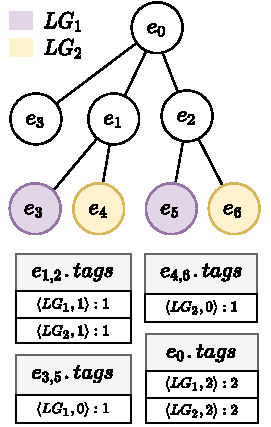
\includegraphics[width=0.5\linewidth]{appstract/explanations/node-tagging}
  \caption{Output of the node-tagging algorithm. Each node is assigned a $tags$ map keeping track of the number of leaf-groups in its offspring.}
  \label{fig:node_tagging}
\end{figure}

An important implementation detail: the above algorithm assumes that the $tag$ tuple's hash code will be generated from the value of its components (and not the object's reference)---\emph{i.e.}, two $tag$ tuples containing the same leaf group $LG$ and the same $depth$ should have the same hash code when inserted into the $e.tags$ map (even though the tags will have different addresses in memory since they were created at a different stage of the algorithm).

\subsubsection{Recursive Branch Merging}
\paragraph{Overview}\label{sec:overview}
The last step of the intra-page abstraction consists in merging all required nodes such that the resulting DOM contains only one node instance of each leaf group. 
Figure~\ref{fig:intra} shows an example of the result obtained after this last step of the intra-page abstraction. 
In the final abstract tree of Figure~\ref{fig:intra}, the red dotted edge connecting the template element $\hat{e}$ to its parent indicates that $\hat{e}$ has a special relationship with its parent, in this case: a 1-to-many relationship.

The algorithm must be recursive because it is possible (and likely) that some leaf groups will have to be merged at different levels of the tree. 
Figure~\ref{fig:intra-use-cases} illustrates this use case: $e_{a1}$ and $e_{a2}$ must be merged first before their ancestor $e_{b1}$ can merge with $e_{b2}$.

\begin{figure}[ht]
  \centering
  \begin{subfigure}{0.4\textwidth}
    \centering
    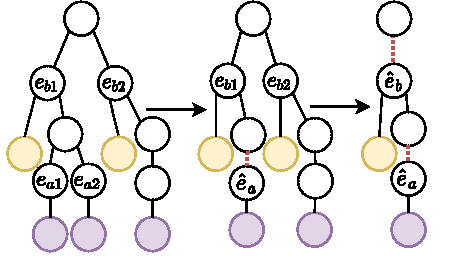
\includegraphics[width=.9\linewidth]{appstract/explanations/intra-recursivity}
    \caption{Nested records}
    \label{fig:nested_records}
  \end{subfigure}
  \begin{subfigure}{0.4\textwidth}
    \centering 
    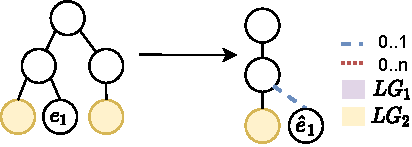
\includegraphics[width=.9\linewidth]{appstract/explanations/intra-optional}
    \caption{Optional elements}
    \label{fig:optional_elements}
  \end{subfigure}
  \caption{Illustrating two important cases our merging algorithm must cover: \emph{nested records} and \emph{optional elements}.}
  \label{fig:intra-use-cases}
\end{figure}

The second case illustrated in Figure~\ref{fig:optional_elements} occurs when merging two nodes even though not all their respective children are merged.
In this case, the inferred abstract node $\hat{e}_1$ is said to have an \textit{optional} relationship with its parent template element---\emph{i.e.}, it only exists as a child node in certain instances of $\hat{e}_1$.
In general, a template element $\hat{e}$ can have many types of relationship with its parent.
In this chapter, we distinguish two relationships:
%% TO revise, it's heavy and probably wrong
\begin{compactitem}
    \item A \emph{zero-to-many relationship} when at least one element from $T^{-1}_e(par(\hat{e})) = par(e_1), par(e_2)...$ has no child element that is an instance of $\hat{e}$ and at least one other element has more than 1,
    \item An \emph{optional (or zero-to-one) relationship} when at least one element from $T^{-1}_e(par(\hat{e})) = par(e_1), par(e_2)...$ has no child element that is an instance of $\hat{e}$ and at least one other element has more than 1.
\end{compactitem}

\paragraph{Algorithm}
Algorithm~\ref{alg:abstractTree} gives a high level view of the solution.
The function \emph{abstractTree} recursively traverses the tree.
For each node $e$ considered, it checks if $e$ is already abstract using the \emph{isAbstract} function (line \ref{alg:abstractTree:isAbstract}).
A node is abstract if none of its children need to be merged.
If $e$ is already abstract then it is returned, otherwise, we:
\begin{compactenum}
  \item recursively call the \emph{abstractTree} function on all children of $e$,
  \item group all abstract children by group of tags using \emph{assocGroup} (see paragraph~\ref{par:assocGroup}), and
  \item merge each group of children using \emph{mergeGroup} (see paragraph~\ref{sec:mergeGroup})
\end{compactenum}

\begin{algorithm}
\caption{Intra-page abstraction: recursive merge}\label{alg:abstractTree}
\begin{algorithmic}[1]
  \Function{abstractTree}{$e: Element$}
    \If {isAbstract($e$)}
      \label{alg:abstractTree:isAbstract}
      \State \Return $e$
    \Else
      \State children $\gets$ $e$.children.map(abstractTree)
      \State children $\gets$ assocGroup(children).map(mergeGroup)
      \State $\hat{e}$ $\gets$ \{ $e$ with $e$.children = children \}
      \State \Return $\hat{e}$
    \EndIf
  \EndFunction
\end{algorithmic}
\end{algorithm}

We describe in details the three functions used in algorithm~\ref{alg:abstractTree}, namely:
\begin{inparaenum}
  \item \emph{isAbstract},
  \item \emph{assocGroup}, and
  \item \emph{mergeGroup}.
\end{inparaenum}

\paragraph{isAbstract}
The function \emph{isAbstract} checks if an element $e$ is already abstract.
An element $e$ is abstract if none of its offsprings need to be merged.
This information is obtained using the tags computed in previous steps (see Section~\ref{sec:node_tagging}).

Each tag $tag$ associated to a node $e$ is associated to its tag count $|tag|$.
Using the tag counts, we can then detect if $e$ is abstract: a node $e$ is abstract iff all tag counts are equal to 1.
In this case, it means that no node in the offspring will have to be merged.
For example, in Figure~\ref{fig:node_tagging}, all nodes are abstract except $e_{0}$ since two tags in $e_{0}.tags$ have a tag count of 2.
In practice, it means that some children of $e_{0}$ (in this case $e_{1}$ and $e_{2}$) will have to be merged.

\paragraph{assocGroup}\label{par:assocGroup}
The function \emph{assocGroup} (for associative grouping) groups all the nodes that need to be merged together.
In order to know if two nodes need to be merged, we look at their associated \emph{tags} map.
The merging condition is simple: two nodes should be merged iff they share one same tag.
Below is an example of input/output pair of the \emph{assocGroup} function:
\begin{lstlisting}
    Input:
        A has t1, t2
        B has t2, t3
        C has t3
        D has t4
        E has t4

    Output:
        [A, B, C] -> [t1, t2, t3]
        [D, E] -> [t4]
\end{lstlisting}

In our case, the letters $A$ to $E$ are nodes and $t1$ to $t4$ are tags.

\paragraph{mergeGroup}\label{par:mergeGroup}
The function \emph{mergeGroup} is the core of the recursive merging algorithm.
As an input, it takes a list of abstract nodes---\emph{i.e.}, abstract subtrees---that need to be merged and the set of common tags between the groups of nodes.
The output is the abstract node $\hat{e}$.
The inputs come from the output of the function \emph{assocGroup}, described above, and the abstract node output replaces all children that were merged in the tree, as shown in the \emph{abstractTree} algorithm~\ref{alg:abstractTree}

The function \emph{mergeGroup} reduces the group list taken as input by repeatedly applying the function \emph{mergeAbstractTrees}.
Algorithm~\ref{alg:mergeAbstractTrees} describes how the function merges two abstract trees into one.

\begin{algorithm}
\caption{Intra-page abstraction: merge two abstract trees}\label{alg:mergeAbstractTrees}
\begin{algorithmic}[1]
  \Function{mergeAbstractTrees}{$\hat{e}_1, \hat{e}_2$}
    \State \Comment{Group pairs of children containing the same tags}
    \State pairs, orphans $\gets$ groupPairs($\hat{e}_1$, $\hat{e}_2$)
    \State mergedChildren $\gets$ pairs.map(mergeAbstractTrees)
    \For{$e$ in orphans}
        \State $e$.rel $\gets$ relType.Optional
    \EndFor
    
    \State $\hat{e}$ $\gets$ new Node()
    \State $\hat{e}$.tag = $\hat{e}$.tag
    \State $\hat{e}$.attrs = mergeAttrs($\hat{e}_1$.attrs, $\hat{e}_2$.attrs)
    \State $\hat{e}$.rel = mergeRel($\hat{e}_1$.rel, $\hat{e}_1$.rel)
    \State $\hat{e}$.children = mergedChildren + orphans
    \State $\hat{e}$.tags = \{$\hat{e}_1 \cup \hat{e}_2$ with tag counts set to 1\}
    \State \Return $\hat{e}$
  \EndFunction
\end{algorithmic}
\end{algorithm}

Before diving into the details of the algorithm, it is important to highlight that the inputs of the function \emph{mergeAbstractTrees} are already abstract.
At this stage of the algorithm, we are assured that along the whole branch starting at the root of both nodes sent as parameters, there is never two children belonging to the same cluster---\emph{i.e.}, that needs to be merged.
It means that the algorithm sole purpose is to recursively merge the two trees between them (and not within).

The function starts by grouping the children of the two nodes into pairs and orphans.
The function \emph{groupPairs} returns two lists: the pairs of nodes that must be merged and the orphan nodes. 
The orphan nodes are the children in $\hat{e_{1/2}}$ that have no corresponding element to be merged with in $\hat{e_{2/1}}$, these elements are set as optional using the \emph{rel} (as in relationship) property.

Before merging, we recursively call the function \emph{mergeAbstractTrees} on each pair of nodes returned by \emph{groupPairs}.
Intuitively, the algorithm will stack the calls to \emph{mergeAbstractTrees} until it reaches the leaves of
the trees, then it will merge the groups of leaves and merge their ancestors as the function calls unstack.

Most of the steps described above help computing the \emph{children} property of the abstract node returned by the \emph{mergeAbstractTrees} function.
Other properties of the nodes are also merged: 
\begin{compactdesc}
\item[\emph{rel}:] In case the relationships of the nodes to merge are different, they are merged using the following pattern matching:
\begin{lstlisting}[basicstyle=\small]
  mergeRelTypes :: (RelType,RelType)->RelType
  mergeRelTypes (t1, t2)
      | (t1, t2) when t1 = t2 -> t1
      | (t1, Normal) -> t1
      | (_, ZeroToMany) -> ZeroToMany
      | (Optional, OneToMany) -> ZeroToMany
      | (t1, t2) -> mergeRelTypes (t2, t1)
\end{lstlisting}

\item[\emph{attrs}:] In case the attributes of the nodes to merge are different, they are merged.
To merge the attributes, we select the attributes that are present in both nodes and merge their values using the \emph{Longest Common Subsequence} (LCS) algorithm.
For example, given three nodes having the following class values:  \emph{class} attribute: \lstinline{"link nav-link"}, \lstinline{"link active nav-link"} and \\\lstinline{"link nav-link"}, the function \emph{mergeAttrs}  will return the following value: \lstinline{"link nav-link"}.
\end{compactdesc}

\paragraph{Stack Diagram}
Since the algorithm has several levels of recursion, it may be hard to understand how a given tree will be abstracted. 

In Figure~\ref{} we describe the different steps of the algorithm.
At each step, we show the output of the current function that is called.
Below each tree, we show the current stack of functions called.

The functions we mention are all described earlier:
\begin{figure}[]
  \centering
  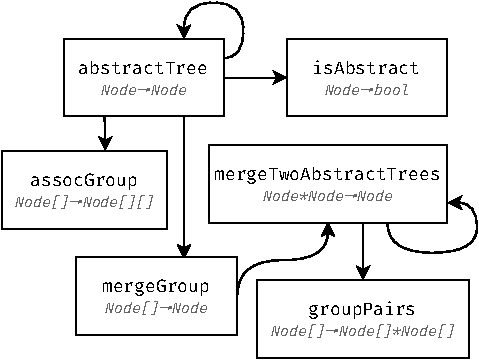
\includegraphics[width=0.7\linewidth]{appstract/explanations/functions_relations}
  \caption{Key functions involved in the \emph{abstractTree} algorithm. A directed arrow from function $f$ to $g$ indicates that $f$ calls $g$.}
  \label{fig:functions_relations}
\end{figure}

\begin{figure*}[]
  \centering
  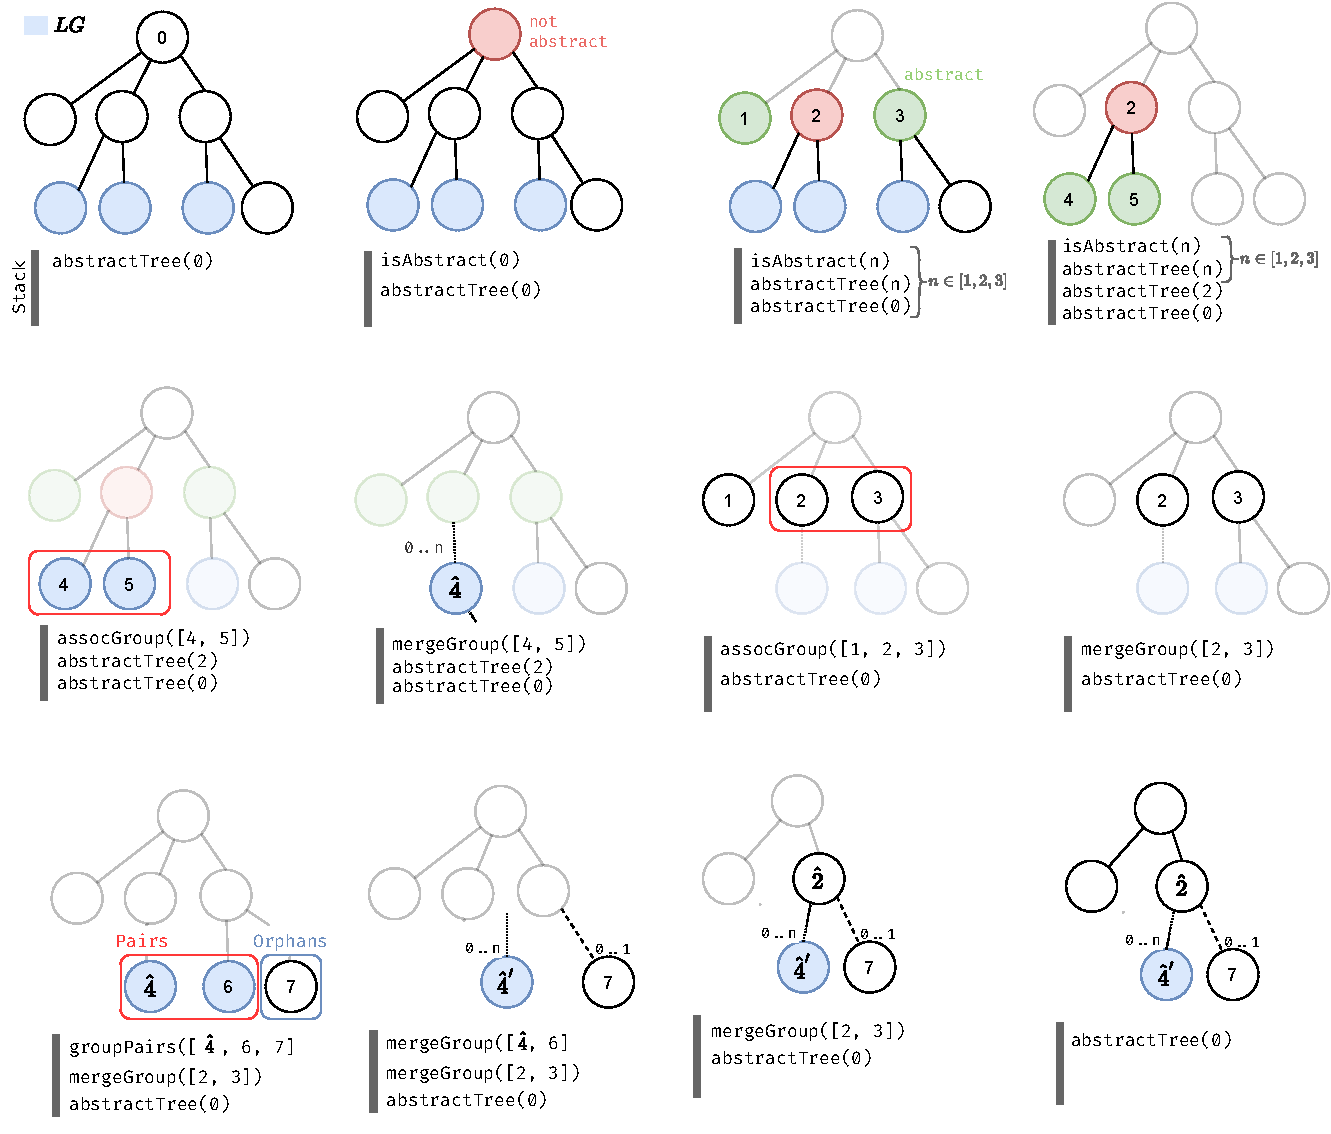
\includegraphics[width=0.8\linewidth]{appstract/explanations/steps_abstractTree}
  \caption{An example application of the \emph{abstractTree} function. For each figure, the stack of the current step is shown below.}
  \label{fig:steps_abstractTree}
\end{figure*}

Figure~\ref{fig:steps_abstractTree} describes an example application of the \emph{abstractTree} function.
At each step, the current stack of functions is shown at the bottom.
All functions shown have been described in the previous sections.
Figure~\ref{fig:functions_relations} summarizes all these functions and how they interact.
For simplicity, however, the \emph{mergeTwoAbstractTrees} is not explicitly mentioned, it is considered as part of the function \emph{mergeGroup}.

% \subsubsection{Complexity}

% \subsubsection{Coordinate System}
% When abstracting, in addition to the application abstraction $A$, we also build a coordinate system to locate each abstracted instance element.
% In order to build our coordinate system, we define the concept of \emph{box}.

% \begin{defn}{Box}
% We call a \textit{box} and we note $\hat{b} \in \hat{A}$ any template element that have a zero to many relationship with their parent.
% \end{defn}

% Every box is associated with a subset several leaf groups

% \emph{Example:}
% ++++Create a figure that shows what a box is.

% Boxes are particularly interesting because they represent record containers. As such they can be used as a useful anchor point to define a coordinate system allowing to locate instances of element templates.

% Let us consider a website containing a list of products. Each product contains a name and a price.
% After abstraction, product names and prices are mapped respectively to the template elements $\hat{e}_{name}$ and $\hat{e}_{price}$.

% Given an input element $e \in p$, the intra-page abstraction allows us to return the corresponding element $T_e(e)$ which means, in our example, either $\hat{e}_{name}$ or $\hat{e}_{price}$. But what if the user of \textsc{Appstract} needs to know which product was clicked on specifically?

% We build a \emph{coordinate system} allowing to locate the instances of any template with regard to their boxes.

% Two approaches are considered:
% \begin{enumerate}
%     \item Complete: coordinates depend on all boxes in the root-to-node path
%     \item Simplified: coordinates depend on the best box selected
% \end{enumerate}

% \emph{Examples.}
% ++++ Coordinates of the examples elements

% A complete coordinate system yields more information but is harder to take advantage of.
% The simplified approach has three main benefits: 
% \begin{enumerate}
% \item The coordinate system is simpler to use because it contains a fixed number of components
% \item Since there are overall less components, more elements will share the same coordinate reference (box).
% \item The box choosing process acts as an important filter for noise
% \end{enumerate}

% \paragraph{Box Choosing as a filter for noise}
% +++ Describe what kind of noise we can have (example: several elements with same paths and they are really a cluster, then one element with the same path but not really a cluster)


% \paragraph{Choosing the best box}
% We study the cases where a Leaf-group is the offspring of several boxes (at different depth).

% Figures.... show some examples.

% Our observation lead us to think that in the majority of cases, a human would not consider all these boxes as valid record containers (for ex....) 

% This observation comes from the fact that in general, it is not super user friendly to expose the user to nested layers of high variability.

% Choosing one only box allows to
% \begin{inparaenum}
%     \item provide more simple abstractions where many elements have the same coordinate base.
% \end{inparaenum}
% That's why we choose to select the best box.

% A "good" box follows the following:
% \begin{itemize}
%     \item It has many instances
%     \item ...
% \end{itemize}

% Voting mecanism:
% \begin{enumerate}
%     \item Each instance $e$ of each leaf-group $LG$ gives one vote for each box on its path.
%     \item Only box templates that account for more than a certain threshold of instances are considered. 
%     \item 
% \end{enumerate}

% \subsubsection{Intra-page abstraction as a Record extractor}
% If we restrict the original (non-abstracted) tree to boxes and text nodes, we get 

% \subsubsection{The algorithm}
% \paragraph{Merging two nodes}

% \subsubsection{Enrich Appstraction}
% In this section, we study how to further enrich the abstraction inferred by Appstract.

% To understand the need for this stage, let us consider the case of a navigation menu containing a set of four links to different sections of the website: home page, products, blog, contact.
% In this situation, it is very likely that the four menu links will be abstracted into one single template link $\hat{e}_{menu link}$.
% Unfortunately, the fact that all menu links are matched to a single template element may be problematic: if \textsc{Appstract} is used to monitor users' activity, then all clicks on the menu will be assimilated to 

\subsection{Inter-Page Abstraction}\label{sec:inter}
We described how to detect and abstract the repeating patterns contained within one page. 
In the second part of the \textsc{Appstract} approach, we detect and abstract repeating patterns across pages of the web application.

The inter-page abstraction relies on tree-matching.
A tree matching solution allows to match two web page DOM trees $p$ and $p'$. 
The matching $M_{p, p'}$ obtained is a subset of  $p \times p'$ such that each tuple $(e, e') \in M_{p, p'}$ represents the fact that the element $e \in p$ matches with the element $e' \in p'$ (e.g. $e$ and $e'$ contain the names of two different products on two different product pages $p$ and $p'$).

As described in Section~\ref{sec:overview}, inter-page abstraction is used at both learning and prediction phases. In both cases, the inter-page abstraction can be described as a function that:
\begin{enumerate}
    \item takes two templates as input: the reference template and a new template,
    \item returns a template in which every template element $\hat{e}$ of the new template references its corresponding template element $\hat{e'}$ in the reference template (if a match was found).
\end{enumerate}

\begin{algorithm}
    \caption{Inter-page abstraction}\label{alg:inter-page}
    \begin{algorithmic}[1]
      \Function{inter}{$\langle p_{ref}, T_{ref} \rangle, \langle p, T \rangle$}
          \State $M \gets$ tree-matching($p$, $p_{ref}$)
          \State $T_{new} \gets$ T.map(($e$, $id$) $\to$ $T_{ref}[M[e]]$ if $e$ in $M$ else $id$)
          \State \Return $\langle p, T_{new} \rangle$
      \EndFunction
    \end{algorithmic}
\end{algorithm}

Algorithm~\label{alg:inter-page} describes the inter-page abstraction process.
The function role is to create a new identifier map $T_{new}$ in which each element from $p$ maps to the id of the matching element in $p_{ref}$ (if there is any) or remains the same.

Figure~\ref{fig:appstract_overview} describes how the function \emph{inter} is used for both learning and prediction:
\begin{compactenum}
    \item during learning, we apply inter-page abstraction between the mother template and each of the other templates. This step allows to build a model of the application where elements that appear in all page templates will have the same id,
    \item during prediction, inter-page abstraction is used to match all elements from an unseen page to the template elements of its matching template page.
\end{compactenum}

\section{Limits}
Modeling a whole application is a highly ambitious task.
We hope our work can help progress toward this goal, but we cannot claim that it already does.
Indeed, our current work has several limits, mainly:

\emph{Template Topology}
Real-life templates may have a much more complex structure than the one we assume:
\begin{enumerate}
\item there can be a tree-like structure with deeply nested templates,
\item there could be graph-like template structure (\emph{e.g.}, components).
\end{enumerate}
Our current \emph{appstraction} method do not allow to infer such template topologies.

\emph{Mother Template Selection}
During the learning stage, we choose the mother template arbitrarily among the existing template pages.
This selection process assumes that all template pages have an equivalent amount of common parts.

\section{Evaluation}\label{sec:evaluation}
In this section, we describe the experiment we devised allowing to evaluate Appstract.
The idea of the experiment is to consider several samples of DOM elements couples and manually judge if they are correctly labeled (should they have the same id?)

\subsection{Experiment}
We intend to measure over- and sub-abstraction rates of Appstract. 
Fundamentally, Appstract allows to create semantically rich, application-wide ids for elements on a webpage.
Where:
\begin{compactitem}
  \item \textit{Semantically Rich} means that two instances of the same template should have the same id
  \item \textit{Application-wide} means that, on a given application instances of a template will have the same id regardless of the page
\end{compactitem}
There are two ways in which Appstract can fail:
\begin{compactitem}
  \item \emph{Over-abstraction}: Items have the same id even though they are not of the same type, or
  \item \emph{Sub-abstraction}: Items have different ids even though a human would assign them the same.
\end{compactitem}
To analyse the performance of Appstract, we thus propose to measure the rates of over- and sub-abstraction.
To do so, we developed a visual way to explore the web page abstractions created by Appstract.
Given an application $A$:
\begin{compactitem}
  \item We apply Appstract to $A$ thus obtaining an abstraction $\langle \hat{A}, T_{\hat{A}} \rangle$
  \item Open two pages $p_{a_1}, p_{a_2}$ that we assume to be instances from the same template $p_a$ (e.g. two product pages or two blog posts)
  \item Use $\langle \hat{A}, T_{\hat{A}} \rangle$ to get the id $T_{\hat{p}}(e) = \hat{e}$ of every element $e$ on both pages $p_{a_1}, p_{a_2}$
  \item Visually display the id $\hat{e}$ when the mouse hovers over an element $e$
\end{compactitem}
This method allows us to simply analyse the results of Appstract.

We separate our experiment into two parts:
\begin{inparaenum}
    \item Over-abstraction and
    \item Sub-abstraction
\end{inparaenum}

\subsubsection{Defining Measures}\label{sec_definition_measures}
After having described what we refer as over-abstraction and sub-abstraction, in this section, we give a formal definitions of these measures.
To do so, we formulate the experimental application of Appstract as a binary classification problem in which each couple of elements between two pages can either have the same locator or a different one.
We then define over-abstraction and sub-abstraction as complementary to the precision and recall of our binary classification problem.

Let us consider two pages $p_1$ and $p_2$ from the same application $A$.
We apply Appstract to $A$ and obtain the abstraction $\langle \hat{A}, T_{\hat{A}} \rangle$.
Then, we apply the abstract model to $p_1$ and $p_2$: 
\begin{align}
T_{\hat{A}}(\hat{p}_1) &= \langle \hat{p_1}, T_{\hat{p_1}} \rangle \\
T_{\hat{A}}(\hat{p}_2) &= \langle \hat{p_2}, T_{\hat{p_2}} \rangle
\end{align}

We formulate the experimental application of Appstract as a binary classification problem.
\begin{defn}[\em Ground Truth Binary Classification function $f$]
\begin{align}
f:  p_1 & \times p_2 \to [0, 1] \\
f(e_1, e_2) &= 1 \text{ if $e_1 \sim e_2$} \\
f(e_1, e_2) &= 0 \text{ otherwise}
\end{align}
where $e_1 \sim e_2$ means that $e_1$ and $e_2$ are instances of the same template element (e.g. a buy button on a product page) as judged by a human.
\end{defn}
$f$ is the ground truth of our experiment. In practice, in the experiment, we only know a small manually labeled sample of $f$.

\begin{defn}[\em Prediction function $\hat{f}$]
\begin{align}
f:  p_1 \times p_2 & \to [0, 1] \\
f(e_1, e_2) &= 1  \text{ if $T_{\hat{p_1}}(e_1) =  T_{\hat{p_2}}(e_2)$}\\
f(e_1, e_2) &= 0 \text{ otherwise}
\end{align}
\end{defn}
$\hat{f}$ is a guess made using Appstract predicting whether two elements should have the same locator.


\begin{defn}[\em Prediction function $\hat{f}$]
\begin{align}
f:  p_1 \times p_2 & \to [0, 1] \\
f(e_1, e_2) &= 1  \text{ if $T_{\hat{p_1}}(e_1) =  T_{\hat{p_2}}(e_2)$}\\
f(e_1, e_2) &= 0 \text{ otherwise}
\end{align}
\end{defn}
Given the above definitions, we can define the traditional precision and recall of our binary classification problem:
\begin{defn}[\em Binary Classification Measures]
\begin{align}
tp &=|\{e_1, e_2 \in p_1, p_2 / f(e_1, e_2) = \hat{f}(e_1, e_2) = 1\}| \\
fp &=|\{e_1, e_2 \in p_1, p_2 / f(e_1, e_2) = 0, \hat{f}(e_1, e_2) = 1\}| \\
fn &=|\{e_1, e_2 \in p_1, p_2 / f(e_1, e_2) = 1, \hat{f}(e_1, e_2) = 0\}| 
\end{align}
where $tp, fp$ and $fn$ stand for true positive, false positive and false negative and |S| is the cardinality of a set $S$.
\begin{align}
precision_{p_1, p_2}(\hat{f}) &= \frac{tp}{tp + fp} \\
recall_{p_1, p_2}(\hat{f})  &= \frac{tp}{tp + fn}
\end{align}
\end{defn}

Finally, we define over-abstraction and sub-abstraction as the complementary measures of precision and recall:
\begin{defn}[\em Over-abstraction rate]
\begin{equation}
o_{p_1, p_2}(\hat{f})  = 1 - precision
\end{equation}
\end{defn}
\begin{defn}[\em Sub-abstraction rate]
\begin{equation}
s_{p_1, p_2}(\hat{f})  = 1 - recall
\end{equation}
\end{defn}

In the next section, we describe an empirical experiment allowing to estimate the over-abstraction and sub-abstraction rates of predictions made by Appstract. 

\subsubsection{Experimental Protocol}
We devise an experimental protocol allowing to evaluate the performance of Appstract on an application.
We separate the experiment into two parts: sub-abstraction and over-abstraction evaluations.
In both experiments, we manually label couples of DOM elements from two pages of the same application.
The idea is to estimate the precision and recall of the function $\hat{f}$ defined in section \ref{sec_definition_measures}.

\paragraph{Selecting couples of pages}
Given an application containing several pages, we need to select a subset of pages couples on which we conduct the experiment.
There are two possibilities:
\begin{enumerate}
    \item Picking random couples
    \item Picking couples of pages that seem to belong to the same template
\end{enumerate}
We choose the second possibility because it provides more relevant data to evaluate.

In the rest of the section, we thus describe the evaluation process on a single couple of DOMs $(p, p')$ belonging to the same template of the same application to which we already applied Appstract. 
Formally, it means we use the functions $T_{\hat{p}}$ and $T_{\hat{p'}}$.

\paragraph{Over-abstraction}
Over-abstraction measures the precision of our algorithm: to how many couple of elements do we mistakenly assign the same id?
More formally:
\begin{equation}
o_{p, p'}(\hat{f}) = 1 - \frac{tp}{tp + fp}
\end{equation}
where $tp$ is the amount of true positives and $fp$ the amount of false positives.

The objective of this part of the experiment is thus to estimate $tp$ and $fp$ given a couple of DOMs $(p, p')$.
Both $tp$ and $fp$ concern the subset of positive couples: the subset of DOM elements couple $(e, e') \in p \times p'$ such that $T_{\hat{p}} = T_{\hat{p'}}$.

To label true and false positives, we develop a script that, given two abstracted web pages $p, p'$:
\begin{enumerate}
\item Display $p$ and $p'$ side by side
\item Highlights one element of each page that have the same id
\item Offer a popup allowing the tester to manually choose between: "Correct", "Wrong" or "Skip"
\end{enumerate}

This experiment allows to estimate the amount of true positives $tp$ ("Correct") and false positives $fp$ ("Wrong").
The "Skip" option is mostly useful in cases where the elements highlighted are not visible.
Results allow us to calculate an estimate of the over-abstraction $\hat{o_{p, p'}}(\hat{f})$

\paragraph{Sub-abstraction}
 Sub-abstraction measures the recall of our algorithm: how many elements should have the same id but do not?
 More formally:
 \begin{equation}
s_{p, p'}(\hat{f}) = 1 - \frac{tp}{tp + fn}
\end{equation}
 To estimate sub-abstraction, we develop a script that, given two abstracted web pages $p, p'$:
\begin{enumerate}
\item Display $p$ and $p'$ side by side
\item Ask the user to select one element from each web page that should have the same id
\item Check if they indeed have the same id. If yes, increment the number of true positive $tp$ else increment the number of false negatives $fn$
\end{enumerate}

We do not disclose the results of the comparison to avoid influencing the following experimenter's choices.

% \paragraph{Building the Dataset}
% Since the labeling is done manually, we can only select a limited set of applications to experiment on.
% We try to choose applications belonging to different categories.

% \subsubsection{Limits}
% As mentioned in Section \ref{sec:introduction}, Appstract opens up many applications, notably in data extraction, analytics or testing. However, testing Appstract indirectly through one of these applications will not provide the same level of precision as the more direct evaluation that we propose. For example, trying to extract data using Appstract requires a lot of additional work that is not directly linked to Appstract (e.g. separating menu items from data records).
% This is the reason why we chose to develop a dedicated evaluation protocol for Appstract.

\subsubsection{Preliminary Results and Limitations}
While we unfortunately did not have enough time to lead the described experiments quantitatively, our first tests of Appstract are promising but show some limitations, mainly related to Free Text detection.
We call \textit{Free Text}, portions of web pages containing text written and, more importantly, formatted by the user. The most significant example of free text is content written on forums or comment sections.  Comment editors on these websites often offer users the option to format (bold, italic, paragraphs...) their text. The formatting tags in free text introduce noise that is difficult to ignore for Appstract. Indeed, the main assumption used by Appstract to separate content from presentation (templates) is that web applications present a high variability of content (text) encoded in a limited amount of templates. In the case of free text, this assumption is false: the structure of the webpage defined through tags is partially written by the user which leads to a high variability of structure since, in this case, the structure is also part of the content. Appstract then mistakenly believes the formatting tags should be used to infer the template which can lead to unexpected results.
To solve the free-text limitation, we need to find a way to detect free text.

\section{Conclusion}\label{sec:conclusion}
We believe Appstract's approach is an important and pioneering solution in two ways.

Firstly, we introduce the webpage abstraction problem independently to its traditional areas of application (e.g. web testing, data extraction, web analytics). We propose a formalisation of the abstraction problem using the idea of robust and semantically-rich application-wide identifiers.

Secondly, we propose an abstraction approach combining intra and inter page abstraction to generate such identifiers. While both intra and inter-page abstraction underlying techniques are akin to existing approaches in different research areas, to our knowledge, the idea to combine both to infer a web application abstraction is original.

The web application abstraction problem we described is very complex, mainly because of the high variety of existing modern web applications. Unfortunately, Appstract is not the off-the-shelf web application abstraction solution working on any application that we intended to develop. Appstract mainly suffers from a lack of quantitative evaluation benchmark and can be mislead by Free Text sections (e.g. comment sections or forum posts). However, we hope it will serve as a starting point to develop new solutions for the web application abstraction problem.
\chapter{Conclusion}
\label{ch:conclusion}

This is the concluding chapter of the thesis.


%%%%%%%%%%%%%%%%%%%%%%%%%%%%%%%%%%%%%



%this is the area for the .bib file
\cleardoublepage
\clearpage
\bibliographystyle{plain}
\bibliography{thesis}
\addcontentsline{toc}{chapter}{Bibliography}
%this adds the Bibliography to the Table of Contents *Note it might 
% be off my one page...this has to be edited manually in the file 
% printing by going into the toc file and changing the numbers.  
% This might be done some other way but I don't know the process...feel 
% free to edit if you find a fix*
\cleardoublepage
\clearpage
\appendix %this is the appendix
\addappheadtotoc %add the appendix to the table of contents
\chapter{Additional Experimental Analysis}


Additional text, raw data, etc., is put into one or more appendices.


\end{document}
